\documentclass[amt]{copernicus}

\begin{document}


\title{Estimates of lightning \chem{NO_\mathit{x}} production based on high-resolution OMI
    \chem{NO_2} retrievals over the continental US}

\Author[1,2]{Xin}{Zhang}
\Author[1,2]{Yan}{Yin}
\Author[2,3]{Ronald}{van der A}
\Author[4]{Jeff}{L. Lapierre}
\Author[1,2]{Qian}{Chen}
\Author[1,2]{Xiang}{Kuang}
\Author[2]{Shuqi}{Yan}
\Author[1,2]{Jinghua}{Chen}
\Author[1,2]{Chuan}{He}
\Author[1,2]{Rulin}{Shi}

\affil[1]{Collaborative Innovation Center on Forecast and Evaluation of Meteorological Disasters/Key Laboratory for Aerosol-Cloud-Precipitation of China Meteorological Administration,
Nanjing University of Information Science and Technology (NUIST), Nanjing 210044, China}
\affil[2]{Department of Atmospheric Physics, Nanjing University of Information Science and Technology (NUIST),\hack{\break} Nanjing 210044, China}
\affil[3]{Royal Netherlands Meteorological Institute (KNMI), Department of Satellite Observations, De Bilt, the Netherlands}
\affil[4]{Earth Networks, Germantown, Maryland, USA}

\runningtitle{Estimates of lightning \chem{NO_\mathit{x}} production}

\runningauthor{X. Zhang et al.}

\correspondence{Yan Yin (yinyan@nuist.edu.cn)}

\received{2 October 2019}
\pubdiscuss{27 November 2019}
\revised{8 March 2020}
\accepted{11 March 2020}
\published{}

\firstpage{1}

\texlicencestatement{This work is distributed under \hack{\newline} the Creative Commons Attribution 4.0 License.}
\maketitle

\begin{abstract}
Lightning serves as the dominant source of nitrogen oxides (\chem{NO_\mathit{x} = NO + NO_2}) in the upper troposphere (UT), with a strong impact on ozone chemistry and the hydroxyl radical production.
However, the production efficiency (PE) of lightning nitrogen oxides (L\chem{NO_\mathit{x}}) is still quite uncertain (32--1100\,mol\,NO per flash).
Satellite measurements are a powerful tool to estimate L\chem{NO_\mathit{x}} directly compared to conventional platforms.
To apply satellite data in both clean and polluted regions, a new algorithm for calculating L\chem{NO_\mathit{x}} has been developed that uses the Berkeley High-Resolution (BEHR) v3.0B \chem{NO_2} retrieval algorithm and the Weather Research and Forecasting model coupled with chemistry (WRF-Chem).
L\chem{NO_\mathit{x}} PE over the continental US is estimated using the \chem{NO_2} product of the Ozone Monitoring Instrument (OMI) data and the Earth Networks Total Lightning Network (ENTLN) data.
Focusing on the summer season during 2014, we find that the lightning \chem{NO_2} (L\chem{NO_2}) PE is $32\pm 15$\,mol\,\chem{NO_2} per flash and $6\pm 3$\,mol\,\chem{NO_2} per stroke while L\chem{NO_\mathit{x}} PE is $ 90 \pm 50$\,mol\,\chem{NO_\mathit{x}} per flash and $17\pm 10$\,mol\,\chem{NO_\mathit{x}} per stroke.
Results reveal that our method reduces the sensitivity to the background \chem{NO_2} and includes much of the below-cloud L\chem{NO_2}.
As the L\chem{NO_\mathit{x}} parameterization varies in studies, the sensitivity of our calculations to the setting of the amount of lightning NO (LNO) is evaluated.
Careful consideration of the ratio of L\chem{NO_2} to \chem{NO_2} is also needed, given its large influence on the estimation of L\chem{NO_2} PE.
\end{abstract}



\introduction


Nitrogen oxides (\chem{NO_\mathit{x}}) near the Earth's surface are mainly produced by soil, biomass burning, and fossil fuel combustion, while \chem{NO_\mathit{x}} in the middle and upper troposphere originates largely from lightning and aircraft emissions.
\chem{NO_\mathit{x}} plays an important role in the production of ozone (\chem{O_3}) and the hydroxyl radical (OH).
While the anthropogenic sources of \chem{NO_\mathit{x}} are largely known, lightning nitrogen oxides (L\chem{NO_\mathit{x}}) are still the source with the greatest uncertainty, though they are estimated to range between 2 and
8\,Tg\,N\,yr$^{-1}$ \citep{Schumann.2007}.
L\chem{NO_\mathit{x}} is produced in the upper troposphere (UT) by \chem{O_2} and \chem{N_2} dissociation in the hot lightning channel as described by the Zel'dovich mechanism \citep{Zeldovich.1967}.
With the recent updates of UT \chem{NO_\mathit{x}} chemistry, the daytime lifetime of UT \chem{NO_\mathit{x}} is evaluated to be $\sim 3$\,h near thunderstorms and $\sim 0.5$--1.5\,d away from thunderstorms \citep{Nault.2016,Nault.2017}.
This results in enhanced \chem{O_3} production in the cloud outflow of active convection \citep{Pickering.1996,Hauglustaine.2001,DeCaria.2005,Ott.2007,Dobber.2008,Allen.2010,Finney.2016}.
As \chem{O_3} is known as a greenhouse gas, strong oxidant, and absorber of ultraviolet radiation \citep{Myhre.2013}, the contributions of L\chem{NO_\mathit{x}} to \chem{O_3} production also have an effect on climate forcing.
\citet{Finney.2018} found different impacts on atmospheric composition and radiative forcing when simulating future lightning using a new upward cloud ice flux (IFLUX) method versus the commonly used cloud-top height (CTH) approach.
While global lightning is predicted to increase by 5\,{\%}--16\,{\%} over the next century with the CTH approach \citep{Clark.2017,Banerjee.2014,Krause.2014}, a 15\,{\%} decrease in global lightning was estimated with IFLUX in 2100 under a strong global warming scenario \citep{Finney.2018}.
As a result of the different effects on radiative forcing from ozone and methane, a net positive radiative forcing was found with the CTH approach while there is little net radiative forcing with the IFLUX approach \citep{Finney.2018}.
However, the convective available potential energy (CAPE) times the precipitation rate ($P$) proxy predicts a $12\pm 5$\,{\%} increase in the continental US (CONUS) lightning strike rate per kelvin of global warming \citep{Romps.2014}, while the IFLUX proxy predicts the lightning will only increase 3.4\,{\%}\,K$^{-1}$  over the CONUS.
Recently, \citet{Romps.2019} compared the CAPE $\times P$ proxy and IFLUX method in cloud-resolving models.
They reported that higher CAPE and updraft velocities caused by global warming could lead to the large increases in tropical lightning simulated by the CAPE $\times P$ proxy, while the IFLUX proxy predicts little change in tropical lightning because of the small changes in the mass flux of ice.

In view of the regionally dependent lifetime of \chem{NO_\mathit{x}} and the difficulty of measuring L\chem{NO_\mathit{x}} directly, a better understanding of the L\chem{NO_\mathit{x}} production is required, especially in the tropical and midlatitude regions in summer.
Using its distinct spectral absorption lines in the near-ultraviolet (UV) and visible (VIS) ranges \citep{Platt.1983}, \chem{NO_2} can be measured by satellite instruments like the Global Ozone Monitoring Experiment \citep[GOME;][]{Burrows.1999, Richter.2005}, SCanning Imaging Absorption SpectroMeter for Atmospheric CHartographY \citep[SCIAMACHY;][]{Bovensmann.1999}, the Second Global Ozone Monitoring Experiment \citep[GOME-2;][]{Callies.2000}, and the Ozone Monitoring Instrument \citep[OMI;][]{Levelt.2006}.
OMI has the highest spatial resolution, least instrument degradation, and longest record among these satellites \citep{Krotkov.2017}.
Satellite measurements of \chem{NO_2} are a powerful tool compared to conventional platforms because of their global coverage, constant instrument features, and temporal continuity.

Recent studies have determined and quantified L\chem{NO_\mathit{x}} using satellite observations.
\citet{Beirle.2004} constrained the L\chem{NO_\mathit{x}} production to 2.8 (0.8--14)\,Tg\,N\,yr$^{-1}$ by combining GOME \chem{NO_2} data and flash counts from the Lightning Imaging Sensor (LIS) aboard the Tropical Rainfall Measurement Mission (TRMM) over Australia.
\citet{Boersma.2005} estimated the global L\chem{NO_\mathit{x}} production of 1.1--6.4\,Tg\,N\,yr$^{-1}$ by comparing GOME \chem{NO_2} with distributions of L\chem{NO_2} modeled by Tracer Model 3 (TM3).
\citet{Martin.2007} analyzed SCIAMACHY \chem{NO_2} columns with Goddard Earth Observing System chemistry model (GEOS-Chem) simulations to identify L\chem{NO_\mathit{x}} production amounting to $6\pm 2$\,Tg\,N\,yr$^{-1}$.

As these methods focus on monthly or annual mean \chem{NO_2} column densities, more recent studies applied specific approaches to investigate L\chem{NO_\mathit{x}} directly over active convection.
\citet{Beirle.2006} estimated L\chem{NO_\mathit{x}} as 1.7 (0.6--4.7)\,Tg\,N\,yr$^{-1}$ based on a convective system over the Gulf of Mexico, using National Lightning Detection Network (NLDN) observations and GOME \chem{NO_2} column densities.
However, it is assumed that all the enhanced \chem{NO_2} originated from lightning and did not consider the contribution of anthropogenic emissions.
\citet{Beirle.2010} analyzed L\chem{NO_\mathit{x}} production systematically using the global dataset of SCIAMACHY \chem{NO_2} observations combined with flash data from the World Wide Lightning Location Network (WWLLN).
Their analysis was restricted to 30\,km\,$\times$\,60\,km satellite pixels where the flash rate exceeded 1\,flash\,km$^{-2}$\,h$^{-1}$.
But they found L\chem{NO_\mathit{x}} production to be highly variable, and correlations between flash-rate densities and L\chem{NO_\mathit{x}} production were low in some cases.
\citet{Bucsela.2010} estimated L\chem{NO_\mathit{x}} production as $\sim 100$--250\,mol\,\chem{NO_\mathit{x}} per flash for four cases, using the DC-8 and OMI data during NASA's Tropical Composition, Cloud and Climate Coupling Experiment (TC4).


Based on the approach used by \citet{Bucsela.2010}, a special algorithm was developed by \citet{Pickering.2016} to retrieve L\chem{NO_\mathit{x}} from OMI and the WWLLN.
The algorithm takes the OMI tropospheric slant column density (SCD) of \chem{NO_2} (S$_\chem{NO_2}$) as the tropospheric slant column density of L\chem{NO_2} (S$_\chem{LNO_2}$) by using cloud radiance fraction (CRF) greater than 0.9 to minimize or screen the lower tropospheric background.
To convert the S$_\chem{LNO_2}$ to the tropospheric vertical column density (VCD) of L\chem{NO_\mathit{x}} (V$_\chem{LNO_\mathit{x}}$), an air mass factor (AMF) is calculated by dividing the a priori S$_\chem{LNO_2}$ by the a priori V$_\chem{LNO_\mathit{x}}$.
The a priori S$_\chem{LNO_2}$ is calculated using a radiative transfer model and a profile of L\chem{NO_2} simulated by the NASA Global Modeling Initiative (GMI) chemical transport model.
The a priori V$_\chem{LNO_\mathit{x}}$ is also obtained from the GMI model.
Results for the Gulf of Mexico during 2007--2011 summer yield L\chem{NO_\mathit{x}} production of $80\pm 45$\,mol\,\chem{NO_\mathit{x}} per flash.
Since they considered \chem{NO_2} above the cloud to be L\chem{NO_2} in the algorithm due to the difficulty and uncertainty in determining the background \chem{NO_2}, their AMF and derived VCD of L\chem{NO_\mathit{x}} (L\chem{NO_2}) are named AMF$_{\chem{LNO_\mathit{x}}\mathrm{Clean}}$ (AMF$_{\chem{LNO_2}\mathrm{Clean}}$) and L\chem{NO_\mathit{x}}Clean (L\chem{NO_2}Clean), respectively.
Note that \citet{Pickering.2016} considered the two estimates of background derived from aircraft flights in the Gulf of Mexico region (3\,{\%} and 33\,{\%}) and subtracted the mean value (18\,{\%}) from the estimated mean L\chem{NO_\mathit{x}} production efficiency (PE) for the background bias.
However, we use the original algorithm directly without correction to distinguish the effect of different AMFs on L\chem{NO_\mathit{x}} estimation in the remainder of this paper.
Unless otherwise specified, abbreviations S and V are respectively defined as the tropospheric SCD and VCD in this paper.

More recently \citet{Bucsela.2019} obtained an average PE of $180\pm 100$\,mol\,\chem{NO_\mathit{x}} per flash over East Asia, Europe, and North America based on a modification of the method used in \citet{Pickering.2016}.
A power function between L\chem{NO_\mathit{x}} and lightning flash rate was established, while the minimum flash-rate threshold was not applied.
The tropospheric \chem{NO_\mathit{x}} background was removed by subtracting the temporal average of \chem{NO_\mathit{x}} at each box where the value was weighted by the number of OMI pixels which meet the optical cloud pressure and CRF criteria required to be considered deep convection but have one flash or fewer instead.
The lofted pollution was considered to be 15\,{\%} of total \chem{NO_\mathit{x}} according to the estimation from \citet{DeCaria.2000,DeCaria.2005}, and the average chemical delay was adjusted by 15\,{\%} following the 3\,h L\chem{NO_\mathit{x}} lifetime in the nearby field of convection \citep{Nault.2017}.
However, there were negative L\chem{NO_\mathit{x}} values caused by the overestimation of the tropospheric background and stratospheric \chem{NO_2} at some locations.

On the other hand, \citet{Lapierre.2020} constrained L\chem{NO_2} to $1.1 \pm 0.2$\,mol\,\chem{NO_2} per stroke for intracloud (IC) strokes and $10.7 \pm 2.5$\,mol\,\chem{NO_2} per stroke for cloud-to-ground (CG) strokes over the CONUS.
L\chem{NO_2} per stroke was scaled to 24.2\,mol\,\chem{NO_\mathit{x}} per flash using mean values of strokes per flash and the ratio of \chem{NO_\mathit{x}} to \chem{NO_2} in the UT.
They used the regridded Berkeley High-Resolution (BEHR) v3.0A $0.05{\degree} \times 0.05{\degree}$ ``visible only'' \chem{NO_2} VCD (V$_\mathrm{vis}$) product which includes two parts of \chem{NO_2} that can be ``seen'' by the satellite.
The first part is the \chem{NO_2} above clouds (pixels with CRF $> 0.9$) and the second part is the \chem{NO_2} detected from cloud-free areas.
A threshold of $3 \times 10^{15}$\,molecules\,cm$^{-2}$, the typical urban \chem{NO_2} concentration, was applied to mask the contaminated grid cells \citep{Beirle.2010,Laughner.2017}.
The main difference between \citet{Lapierre.2020} and \citet{Pickering.2016} is the air mass factor for lightning (AMF$_\chem{LNO_\mathit{x}}$) implemented in the basic algorithm.
In \citet{Lapierre.2020}, the air mass factor was used to convert S$_\chem{NO_2}$ to V$_\mathrm{vis}$, while in \citet{Pickering.2016} it was used to convert S$_\chem{LNO_2}$ to V$_\chem{LNO_\mathit{x}}$, assuming that all S$_\chem{NO_2}$ is generated by lightning.

To apply the approach used by \citet{Bucsela.2010}, \citet{Pickering.2016}, \citet{Bucsela.2019}, and \citet{Lapierre.2020} without geographic restrictions, the contamination by anthropogenic emissions must be taken into account in detail.
The Weather Research and Forecasting (WRF) model coupled with chemistry (WRF-Chem) has been employed to evaluate the convective transport and chemistry in many studies \citep{Barth.2012,Wong.2013,Fried.2016,Li.2017}.
Meanwhile, \citet{Laughner.2017} showed that the OMI AMF is increased by $\sim35\,{\%}$ for summertime when L\chem{NO_2} simulated by WRF-Chem is included in the a priori profiles to match aircraft observations.
The simulation agrees with observed \chem{NO_2} profiles and the bias of AMF related to these observations is reduced to $< \pm4$\,{\%} for OMI viewing geometries.

In this paper, we focus on the estimation of L\chem{NO_2} production per flash (L\chem{NO_2} per flash), L\chem{NO_\mathit{x}} production per flash (L\chem{NO_\mathit{x}} per flash), L\chem{NO_2} production per stroke (L\chem{NO_2} per stroke), and L\chem{NO_\mathit{x}} production per stroke (L\chem{NO_\mathit{x}} per stroke) in May--August (MJJA) 2014 by developing an algorithm similar to that of \citet{Pickering.2016} based on the BEHR \chem{NO_2} retrieval algorithm \citep{Laughner.2018,Laughner.2019}, but it performs better over background \chem{NO_2} sources.
Section~\ref{section:DataandMethods} describes the satellite data, lightning data, model settings, and the algorithm in detail.
Section~\ref{section:Results} explores the suitable data criteria, compares different methods, and evaluates the effect of background \chem{NO_2}, cloud, and L\chem{NO_\mathit{x}} parameterization on L\chem{NO_\mathit{x}} production estimation.
Section~\ref{section:Uncertainties} examines the effect of different sources of the uncertainty on the results.
Conclusions are summarized in Sect.~\ref{section:conclusions}.

\section{Data and methods} \label{section:DataandMethods}

\subsection{Ozone Monitoring Instrument (OMI)}

OMI is carried on the Aura satellite (launched in 2004), a member of the A-train satellite group \citep{Levelt.2006,Levelt.2018}. OMI passes over the Equator at $\sim 13$:45\,LT (ascending node) and has a swath width of 2600\,km, with a nadir field-of-view resolution of 13\,km\,$\times$\,24\,km.
Since the beginning of 2007, some of the measurements have become useless as a result of anomalous radiances called the ``row anomaly'' \citep{Dobber.2008,KNMI.2020}.
For the current study, we used the NASA standard product v3.0 \citep{Krotkov.2017} as input to the L\chem{NO_\mathit{x}} retrieval algorithm.

The main steps of calculating the \chem{NO_2} tropospheric VCD (V$_\chem{NO_2}$) in the NASA product include the following.
\begin{enumerate}
\item SCDs are determined by the OMI-optimized differential optical absorption spectroscopy (DOAS) spectral fit.

\item A corrected (``de-striped'') SCD is obtained by subtracting the cross-track bias caused by an instrument artifact from the measured slant column.

\item The AMF for stratospheric (AMF$_\mathrm{strat}$) or tropospheric column (AMF$_\mathrm{trop}$) is calculated from the \chem{NO_2} profiles integrated vertically using weighted scattering weights with the a priori profiles. These profiles are obtained from GMI monthly mean profiles using 4 years (2004--2007) of simulation.

\item The stratospheric \chem{NO_2} VCD (V$_\mathrm{strat}$) is calculated from the subtraction of the a priori contribution from tropospheric \chem{NO_2} and a three-step (interpolation, filtering, and smoothing) algorithm  \citep{Bucsela.2013}.

\item V$_\mathrm{strat}$ is converted to the slant column using AMF$_\mathrm{strat}$ and subtracted from the measured SCDs to yield S$_\chem{NO_2}$, leading to V$_\chem{NO_2} =$ S$_\chem{NO_2}$/AMF$_\mathrm{trop}$.

Based on this method, we developed a new AMF$_\chem{LNO_\mathit{x}}$ to obtain the desired V$_\chem{LNO_\mathit{x}}$ (V$_\chem{LNO_\mathit{x}} =$ S$_\chem{NO_2}$/AMF$_\chem{LNO_\mathit{x}}$) by replacing the original step. \item
Details of this algorithm are discussed in Sect.~\ref{section:AMF}.
\end{enumerate}

\subsection{The Earth Networks Total Lightning Detection Network (ENTLN)}
The Earth Networks Total Lightning Network (ENTLN) operates a system of over 1500 ground-based stations around the world with more than 900 sensors installed in the CONUS \citep{Zhu.2017}.
Both IC and CG lightning flashes are located by the sensors with detection frequency ranging from 1\,Hz to 12\,MHz based on the electric field pulse polarity and wave shapes.
Groups of pulses are classified as a flash if they are within 700\,ms and 10\,km.
In the preprocessed data obtained from the ENTLN, both strokes and lightning flashes composed of one or more strokes are included.

\citet{Rudlosky.2015} compared ENTLN combined events (IC and CG) with LIS flashes and found that the relative flash detection efficiency of ENTLN over CONUS increases from 62.4\,{\%} during 2011 to 79.7\,{\%} during 2013.
\citet{Lapierre.2020} also compared combined ENTLN and the NLDN dataset with data from the LIS during 2014 and found the detection efficiencies of IC flashes and strokes to be 88\,{\%} and 45\,{\%}, respectively.
Since we only use the ENTLN data in 2014 as \citet{Lapierre.2020}, and NLDN detection efficiency of IC pulses should be lower than 33\,{\%}, which is calculated by the data in 2016 \citep{Zhu.2016}, only the IC flashes and strokes are divided by 0.88 and 0.45, respectively, while CG flashes and strokes are unchanged because of the high detection efficiency.

\subsection{Model description}
The present study uses WRF-Chem version 3.5.1 \citep{Grell.2005} with a horizontal grid size of 12\,km\,$\times$\,12\,km and 29 vertical levels (Fig.~\ref{fig:domain}).
The initial and boundary conditions of meteorological parameters are provided by the North American Regional Reanalysis (NARR) dataset with a 3-hourly time resolution.
Based on \citet{Laughner.2019}, 3D wind fields, temperature, and water vapor are nudged towards the NARR data.
Outputs from version 4 of the Model for Ozone and Related chemical Tracers \citep[MOZART-4;][]{Emmons.2010} are used to generate the initial and boundary conditions of chemical species.
Anthropogenic emissions are driven by the 2011 National Emissions Inventory (NEI), scaled to model years by the Environmental Protection Agency annual total emissions \citep{EPA.2015}.
The Model of Emissions of Gases and Aerosol from Nature \citep[MEGAN;][]{Guenther.2006} is used for biogenic emissions.
The chemical mechanism is version 2 of the Regional Atmospheric Chemistry Mechanism \citep[RACM2;][]{Goliff.2013} with updates from \citet{Browne.2014} and \citet{Schwantes.2015}.
In addition, lightning flash rate based on the level of neutral buoyancy parameterization \citep{Price.1992,Wong.2013} and L\chem{NO_\mathit{x}} parameterizations is activated (200\,mol\,NO per flash, the factor to adjust the predicted number of flashes is set to 1, hereinafter referred to as ``$1\times200$\,mol\,NO per flash'').
Simulated total flash densities are higher than ENTLN observations over the southeast US and lower than observations in the north-central US (Fig.~\ref{fig:TL}).
The impact of these biases on L\chem{NO_\mathit{x}} production is discussed and mitigated in Sect.~\ref{section:Criteria} and~\ref{section:Effectsofcloud}.
The bimodal profile modified from the standard \citet{Ott.2010} profile \citep{Laughner.2017} is employed as the vertical distribution of lightning NO (LNO) in WRF-Chem, while outputs of LNO and L\chem{NO_2} profiles are defined as the difference of vertical profiles between simulations with and without lightning.

%f1
\begin{figure}[t]
    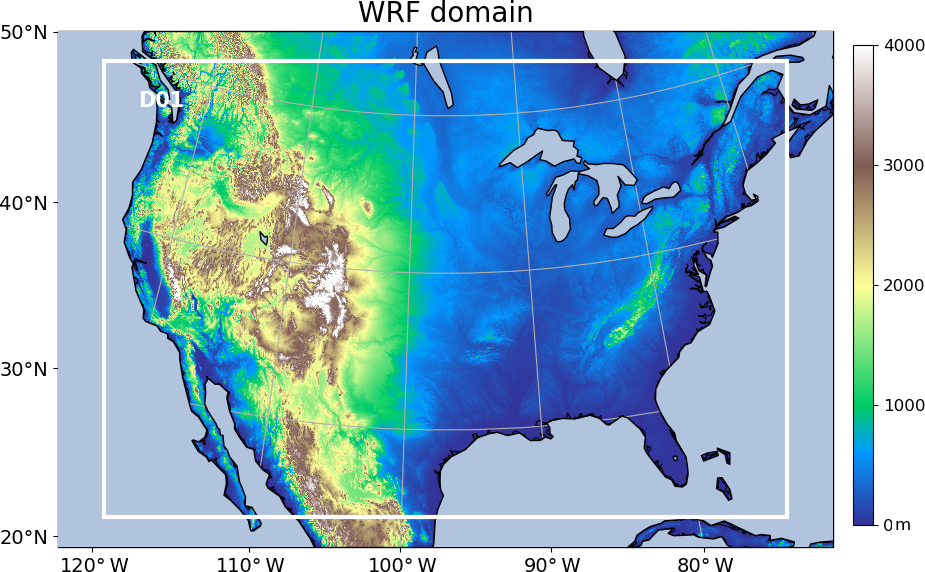
\includegraphics[width=8.3cm]{amt-2019-372-f01.png}
    \caption{Domain and terrain height (m) of the WRF-Chem simulation with $350 \times 290$ grid cells and a horizontal resolution of 12\,km.}
    \label{fig:domain}
\end{figure}

%f2
\begin{figure*}[t]
    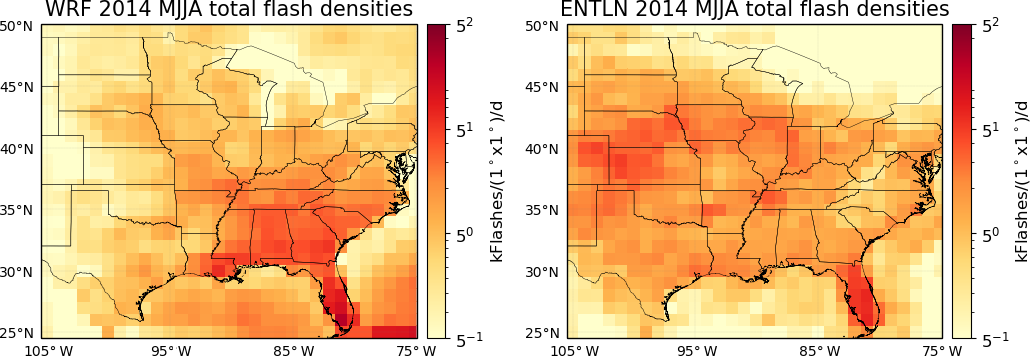
\includegraphics[width=12cm]{amt-2019-372-f02.png}
    \caption{Comparison between total flash densities from ENTLN and WRF-Chem during MJJA 2014.}
    \label{fig:TL}
\end{figure*}

\subsection{Method for deriving AMF} \label{section:AMF}
The V$_\chem{LNO_\mathit{x}}$ near convection is calculated according to
\begin{equation}
\mathrm{V}_\chem{LNO_\mathit{x}} = \frac{\mathrm{S}_\chem{NO_2}}{\mathrm{AMF}_\chem{LNO_\mathit{x}}},
\end{equation}
where S$_\chem{NO_2}$ is the OMI-measured tropospheric slant column \chem{NO_2}, and AMF$_\chem{LNO_\mathit{x}}$ is a customized lightning air mass factor.
The concept of AMF$_\chem{LNO_\mathit{x}}$ was also used in \citet{Beirle.2009} to investigate the sensitivity of satellite instruments to freshly produced lightning \chem{NO_\mathit{x}}.
In order to estimate L\chem{NO_\mathit{x}}, we define the AMF$_\chem{LNO_\mathit{x}}$ as the ratio of the ``visible'' modeled \chem{NO_2} slant column to the total modeled tropospheric L\chem{NO_\mathit{x}} vertical column (derived from the a priori NO and \chem{NO_2} profiles, scattering weights, and cloud radiance fraction):
\begin{equation} \label{AMFLNOx}
\mathrm{AMF}_{\chem{LNO_\mathit{x}}} = \displaystyle{{(1-f_\mathrm{r}) \int_{p_\mathrm{surf}}^{p_\mathrm{tp}} w_\mathrm{clear}(p) \chem{NO_2}(p) \: \mathrm{d}p \atop + f_\mathrm{r} \int_{p_\mathrm{cloud}}^{p_\mathrm{tp}} w_\mathrm{cloudy}(p) \chem{NO_2}(p) \: \mathrm{d}p} \over{\int_{p_\mathrm{surf}}^{p_\mathrm{tp}} \chem{LNO_\mathit{x}}(p) \: \mathrm{d}p}},
\end{equation}
where $f_\mathrm{r}$ is the cloud radiance fraction (CRF), $p_\mathrm{surf}$ is the surface pressure, $p_\mathrm{tp}$ is the tropopause pressure, $p_\mathrm{cloud}$ is the cloud optical pressure (CP), $w_\mathrm{clear}$ and $w_\mathrm{cloudy}$ are respectively the pressure-dependent scattering weights from the TOMRAD lookup table \citep{Bucsela.2013} for clear and cloudy parts, and \chem{NO_2}$(p)$ is the modeled \chem{NO_2} vertical profile. Details of these standard parameters and calculation methods are given in \citet{Laughner.2018}.
L\chem{NO_\mathit{x}}$(p)$ is the L\chem{NO_\mathit{x}} vertical profile calculated by the difference of vertical profiles between WRF-Chem simulations with and without lightning.

Please note that the CP is a reflectance-weighted pressure retrieved by the collision-induced \chem{O_2}--\chem{O_2} absorption band near 477\,nm \citep{Acarreta.2004,Sneep.2008,Stammes.2008}.
For a deep convective cloud with lightning, the CP lies below the geometrical cloud top, which is much closer to that detected by thermal infrared sensors, such as CloudSat and the Aqua Moderate Resolution Imaging Spectrometer (MODIS) \citep{Vasilkov.2008,Joiner.2012}.
Hence, much of the tropospheric \chem{NO_2} measured by OMI lies inside the cloud rather than above the cloud top.
In the following, ``above cloud'' or ``below cloud'' is relative to the cloud pressure detected by OMI.
The sensitivity study of \citet{Beirle.2009} compared the chemical composition from the cloud bottom to that of the cloud top and revealed that a significant fraction of the \chem{NO_2} within the cloud originating from lightning can be detected by the satellite.
This valuable cloud pressure concept has been applied not only in the L\chem{NO_\mathit{x}} research but also in the cloud slicing method of deriving the UT \chem{O_3} and \chem{NO_\mathit{x}} \citep{Ziemke.2009,Ziemke.2017,Choi.2014,Strode.2017,Marais.2018}.
As discussed in \citet{Pickering.2016}, the ratio of V$_\chem{LNO_2}$ seen by OMI to V$_\chem{LNO_\mathit{x}}$ is partly influenced by $p_\mathrm{cloud}$.
The effects of LNO$_2$ below the cloud will be discussed in Sect.~\ref{section:Effectsofcloud}.

To compare our results with those of \citet{Pickering.2016} and \citet{Lapierre.2020}, we calculate their AMF$_{\chem{LNO_\mathit{x}}\mathrm{Clean}}$ and AMF$_{\chem{NO_2}\mathrm{Vis}}$, respectively:
\begin{gather}
\mathrm{AMF}_{\chem{LNO_\mathit{x}}\mathrm{Clean}} = \displaystyle{{(1-f_\mathrm{r}) \int_{p_{\mathrm{surf}}}^{p_{\mathrm{tp}}} w_\mathrm{{clear}}(p) \chem{LNO_2}(p) \: \mathrm{d}p \atop + f_\mathrm{r} \int_{p_\mathrm{{cloud}}}^{p_{\mathrm{tp}}} w_{\mathrm{cloudy}}(p) \chem{LNO_2}(p) \: \mathrm{d}p}\over{\int_{p_{\mathrm{surf}}}^{p_{\mathrm{tp}}} \chem{LNO_\mathit{x}}(p) \: \mathrm{d}p}},\\
\mathrm{AMF}_{\chem{NO_2}\mathrm{Vis}} = \displaystyle{{(1-f_\mathrm{r}) \int_{p_{\mathrm{surf}}}^{p_{\mathrm{tp}}} w_\mathrm{{clear}}(p) \chem{NO_2}(p) \: \mathrm{d}p \atop+ f_\mathrm{r} \int_{p_\mathrm{{cloud}}}^{p_{\mathrm{tp}}} w_{\mathrm{cloudy}}(p) \chem{NO_2}(p) \: \mathrm{d}p}\over{(1-f_\mathrm{g}) \int_{p_{\mathrm{surf}}}^{p_{\mathrm{tp}}} \chem{NO_2}(p) \: \mathrm{d}p \atop+ f_\mathrm{g} \int_{p_\mathrm{{cloud}}}^{p_{\mathrm{tp}}} \chem{NO_2}(p) \: \mathrm{d}p}},
\end{gather}
where $f_\mathrm{g}$ is the geometric cloud fraction and L\chem{NO_2}$(p)$ is the modeled L\chem{NO_2} vertical profile.
Besides these AMFs, another AMF called AMF$_{\chem{LNO_2}\mathrm{Vis}}$ is developed for later comparison.
\begin{equation}
\mathrm{AMF}_{\chem{LNO_2}\mathrm{Vis}} = \displaystyle{{(1-f_\mathrm{r}) \int_{p_{\mathrm{surf}}}^{p_{\mathrm{tp}}} w_\mathrm{{clear}}(p) \chem{NO_2}(p) \: \mathrm{d}p \atop+ f_\mathrm{r} \int_{p_\mathrm{{cloud}}}^{p_{\mathrm{tp}}} w_{\mathrm{cloudy}}(p) \chem{NO_2}(p) \: \mathrm{d}p}\over{(1-f_\mathrm{g}) \int_{p_{\mathrm{surf}}}^{p_{\mathrm{tp}}} \chem{LNO_2}(p) \: \mathrm{d}p\atop + f_\mathrm{g} \int_{p_\mathrm{{cloud}}}^{p_{\mathrm{tp}}} \chem{LNO_2}(p) \: \mathrm{d}p}}
\end{equation}
A full definition list of the used AMFs is shown in Appendix~\ref{AppendixA}.

\subsection{Procedures for deriving L\chem{NO_\mathit{x}}} \label{section:Conditions}

V$_\chem{LNO_\mathit{x}}$ is re-gridded to $0.05{\degree}\times 0.05{\degree}$ grids using the constant value method \citep{Kuhlmann.2014}.
Then, it is analyzed in $1{\degree}\times 1{\degree}$ grid boxes with a minimum of 50 valid $0.05{\degree}\times 0.05{\degree}$ grids to minimize the noise.
The main procedures of deriving L\chem{NO_\mathit{x}} are as follows.

CRFs (CRF~$\geq 70$\,{\%}, CRF~$\geq 90\,{\%}$, and CRF~$= 100\,{\%}$) and CP~$\leq 650$\,hPa are various criteria of deep convective clouds for OMI pixels \citep{Ziemke.2009,Choi.2014,Pickering.2016}.
The effect of different CRFs on the retrieved L\chem{NO_\mathit{x}} is explored in Sect.~\ref{section:Comparison}.
Furthermore, another criterion of cloud fraction (CF) is applied to the WRF-Chem results for the successful simulation of convection.
The CF is defined as the maximum cloud fraction calculated by the Xu--Randall method between 350 and 400\,hPa \citep{Xu.1996,Strode.2017}.
This atmospheric layer (between 350 and 400\,hPa) avoids any biases in the simulation of high clouds.
We choose CF~$\geq 40\,{\%}$ suggested by \citet{Strode.2017} to determine cloudy or clear for each simulation grid.

Besides cloud properties, a time period and sufficient flashes (or strokes) are required for fresh L\chem{NO_\mathit{x}} to be detected by OMI.
The time window ($t_\mathrm{window}$) is the hours prior to the OMI overpass time.
$t_\mathrm{window}$ is limited to 2.4\,h by the mean wind speed at pressure levels 500--100\,hPa during OMI overpass time and the square root of the $1{\degree}\times 1{\degree}$ box over the CONUS \citep{Lapierre.2020}.
Meanwhile, 2400\,flashes per box and 8160\,strokes per box per 2.4\,h time window are chosen as sufficient for detecting L\chem{NO_\mathit{x}} \citep{Lapierre.2020}.
These criteria will result in a low bias in the PE results, as \citet{Bucsela.2019} found that the PE is larger at small flash rates, which are discarded here.
Since our study focuses on developing a new AMF and compares results with other works using similar lightning thresholds \citep{Lapierre.2020,Pickering.2016}, we will only discuss results based on the strict criteria in the main text.
For comparisons between the criterion of 2400 flashes per box and that of one flash per box, scatter diagrams using different lightning criteria are presented in Appendix~\ref{AppendixB}.

To ensure that lightning flashes are simulated successfully by WRF-Chem, the threshold of simulated total lightning flashes (TL) per box is set to 1000, which is fewer than that used by the ENTLN lightning observation, considering the uncertainty of lightning parameterization.
In view of other \chem{NO_2} sources in addition to L\chem{NO_2}, the ratio of modeled lightning \chem{NO_2} above cloud (L\chem{NO_2}Vis) to modeled \chem{NO_2} above cloud (\chem{NO_2}Vis) is defined to check whether enough L\chem{NO_2} can be detected by OMI.
The ratio $\geq 50$\,{\%} indicates that more than half of the \chem{NO_\mathit{x}} above the cloud must have an L\chem{NO_\mathit{x}} source.

Finally, the \chem{NO_2} lifetime due to oxidation should be taken into account.
As estimated by \citet{Nault.2017}, the lifetime ($\tau$) of \chem{NO_2} in the near field of convections is $\sim$ 3\,h.
The initial value of \chem{NO_2} is solved by Eq.~(\ref{inition}) as
\begin{equation} \label{inition}
\chem{NO_2}(0) = \chem{NO_2}(\mathrm{OMI}) \times e^{0.5t/\tau},
\end{equation}
where \chem{NO_2(0)} is the moles of \chem{NO_2} emitted at time $t = 0$, \chem{NO_2}(OMI) is the moles of \chem{NO_2} measured at the OMI overpass time, and $0.5t$ is the half cross grid time, which is 1.2\,h, assuming that lightning occurred at the center of each $1{\degree}\times 1{\degree}$ box.
For each grid box, the mean L\chem{NO_\mathit{x}} vertical column is obtained by averaging V$_\chem{LNO_\mathit{x}}$ values from all regridded $0.05{\degree}\times 0.05{\degree}$ pixels in the box.
This mean value is converted to moles of L\chem{NO_\mathit{x}} using the dimensions of the grid box.
Two methods are applied to estimate the seasonal mean L\chem{NO_2} per flash, L\chem{NO_\mathit{x}} per flash, L\chem{NO_2} per stroke, and L\chem{NO_\mathit{x}} per stroke:
\begin{enumerate}
\item summation method, dividing the sum of L\chem{NO_\mathit{x}} by the sum of flashes (or strokes) in each $1{\degree}\times 1{\degree}$ box in MJJA 2014;

\item linear regression method, applying the linear regression to daily mean values of L\chem{NO_\mathit{x}} and flashes (or strokes).
\end{enumerate}

\section{Results} \label{section:Results}
\subsection{Criteria determination} \label{section:Criteria}
To determine the suitable criteria from the conditions defined in Sect.~\ref{section:Conditions}, six different combinations are defined (Table~\ref{table:Abbreviations}) and applied to the original data with a linear regression method (Table~\ref{table:conditions}).

%t1
\begin{table*}[t]
\caption{Definitions of the abbreviations for the criteria used in this study.}\scalebox{.98}[.98]{
\begin{tabular}{ll}
\tophline
{Abbreviations} & {Full form (source)} \\
\middlehline
CRF                             & Cloud radiance fraction (OMI) \\
CP                              & Cloud optical pressure (OMI) \\
CF                              & Cloud fraction (WRF-Chem) \\
TL                              & Total lightning flashes (WRF-Chem) \\
Ratio                           & Modeled L\chem{NO_2}Vis / modeled \chem{NO_2}Vis (WRF-Chem) \\
CRF$\alpha$\_ENTLN                    & CRF $\geq \alpha +$ ENTLN flashes (strokes) $\geq 2400$ (8160) (ENTLN)\\
CRF$\alpha$\_CF40\_ENTLN              & CRF $\geq \alpha +$ ENTLN flashes (strokes) $\geq 2400$ (8160) $+$ CF $\geq 40$\,{\%} \\
CRF$\alpha$\_ENTLN\_TL1000            & CRF $\geq \alpha +$ ENTLN flashes (strokes) $\geq 2400$ (8160) $+$ TL $\geq 1000$ \\
CRF$\alpha$\_CF40\_ENTLN\_TL1000      & CRF $\geq \alpha +$ ENTLN flashes (strokes) $\geq 2400$ (8160) $+$ CF $\geq 40\,{\%} +$ TL $\geq$ 1000 \\
CRF$\alpha$\_ENTLN\_TL1000\_ratio50   & CRF $\geq \alpha +$ ENTLN flashes (strokes) $\geq2400$ (8160) $+$ TL $\geq 1000 +$ ratio $\geq$ 50\,{\%} \\
CRF$\alpha$\_CF40\_ENTLN\_TL1000\_ratio50 & CRF $\geq \alpha +$ ENTLN flashes (strokes) $\geq 2400$ (8160) $+$ CF $\geq 40$\,{\%} $+$ TL $\geq 1000 +$ ratio $\geq 50$\,{\%} \\
CRF$\alpha$\_ENTLN1(3.4)\_TL1\_ratio50    & CRF $\geq \alpha$ + ENTLN flashes (strokes) $\geq 1$ (3.4) $+$ TL $\geq 1 +$ ratio $\geq 50$\,{\%} \\
\bottomhline
\end{tabular}}
\scalebox{.98}[.98]{\belowtable{$\alpha$ has three options: 70\,{\%}, 90\,{\%}, or 100\,{\%}.}}
\label{table:Abbreviations}
\end{table*}

%t2
\begin{table*}[t]
    \caption{L\chem{NO_\mathit{x}} production efficiencies for different combinations of criteria defined in Table~\ref{table:Abbreviations}.}
    \begin{tabular}{llrrrr}
        \tophline
        {Condition$^1$} & {ENTLN data} & {L\chem{NO_\mathit{x}} per flash or } & {$R$ value} & {Intercept} & {Days$^3$} \\

         &type$^2$ &L\chem{NO_\mathit{x}} per stroke & &(10$^{6}$\,mol) &\\

        \middlehline
        CRF90\_ENTLN                        & Flash  & $52.1 \pm 51.1$ & 0.20 & 0.21  & 99 \\
        CRF90\_CF40\_ENTLN                  & Flash  & $84.2 \pm 31.5$ & 0.54 & $-0.04$ & 70 \\
        CRF90\_ENTLN\_TL1000                & Flash  & $61.9 \pm 49.1$ & 0.27 & 0.33  & 83 \\
        CRF90\_CF40\_ENTLN\_TL1000          & Flash  & $63.4 \pm 52.9$ & 0.38 & 0.26  & 38 \\
        CRF90\_ENTLN\_TL1000\_ratio50       & Flash  & $54.5 \pm 48.1$ & 0.25 & 0.39  & 81 \\
        CRF90\_CF40\_ENTLN\_TL1000\_ratio50 & Flash  & $90.0 \pm 65.0$ & 0.46 & 0.15  & 32 \\
        CRF90\_ENTLN                        & Stroke & $ 6.7 \pm 4.1 $& 0.31 & 0.23  & 102 \\
        CRF90\_CF40\_ENTLN                  & Stroke & $10.3 \pm 3.6 $& 0.55 & 0.08 & 79 \\
        CRF90\_ENTLN\_TL1000                & Stroke & $7.5 \pm 5.1$ & 0.29 & 0.38  & 94 \\
        CRF90\_CF40\_ENTLN\_TL1000          & Stroke & $8.6 \pm 6.2$ & 0.39 & 0.27  & 46 \\
        CRF90\_ENTLN\_TL1000\_ratio50       & Stroke & $7.0 \pm 4.8$ & 0.29 & 0.42  & 93 \\
        CRF90\_CF40\_ENTLN\_TL1000\_ratio50 & Stroke & $8.9 \pm 7.0$ & 0.39 & 0.31  & 40 \\
        \bottomhline
    \end{tabular}
    \belowtable{$^1$~These conditions are defined in Table~\ref{table:Abbreviations}. $^2$~The thresholds of ENTLN data are 2400 flashes per box and 8160 strokes per box during the period of 2.4\,h before OMI overpass time. $^3$~The number of valid days with specific criteria in MJJA 2014.}
    \label{table:conditions}
\end{table*}

A daily search of the \chem{NO_2} product for coincident ENTLN flash (stroke) data results in 99 (102) valid days under the CRF90\_ENTLN condition.
Taking the flash-type ENTLN data as an example, the number of valid days decreases from 99 to 81 under the CRF90\_ENTLN\_TL1000\_ratio50 condition, while L\chem{NO_\mathit{x}} per flash increases from $52.1\pm 51.1$ to $54.5\pm 48.1$\,mol per flash.
The result is almost the same as that under the CRF90\_ENTLN\_TL1000 condition, which is without the condition of more than half of the above-cloud \chem{NO_\mathit{x}} having an L\chem{NO_\mathit{x}} source.
Although this indicates the criterion of TL works well, it is better to include the ratio criterion in case there are some exceptions in the different AMF methods.
Since CF $\geq 40$\,{\%} leads to a sharp loss of valid numbers and production, it is not a suitable criterion.
Instead the CRF criteria are used.
Finally, coincident ENTLN data, TL $\geq 1000$, and ratio $\geq 50$\,{\%} are chosen as the thresholds to explore the effects of three different CRF conditions (CRF~$\geq 70\,{\%}$, CRF $\geq 90$\,{\%}, and CRF~$= 100$\,{\%}) on L\chem{NO_\mathit{x}} production (Table~\ref{table:CRFs}).
Apart from the fewer valid days under higher CRF conditions (CRF~$\geq 90\,{\%}$ and CRF~$= 100$\,{\%}), L\chem{NO_\mathit{x}} per flash increases from $35.7 \pm 36.8$ to 54.5 $\pm$ 48.1\,mol per flash and decreases again to $20.8 \pm 37.4$\,mol per flash while L\chem{NO_\mathit{x}} per stroke enhances from $4.1  \pm 3.9 $ to $7.0\pm 4.8$\,mol per stroke and drops again to $2.6 \pm 4.0$\,mol per stroke (Table~\ref{table:CRFs}), as the CRF criterion increases from 70\,{\%} to 90\,{\%} and to 100\,{\%}.
When the CRF increases from 90\,{\%} to 100\,{\%}, the L\chem{NO_\mathit{x}} PE decreases because of the higher lightning density with less L\chem{NO_\mathit{x}} (not shown).
The increment of L\chem{NO_\mathit{x}} PE caused by the CRF increase from 70\,{\%} to 90\,{\%} is opposite to the result of \citet{Pickering.2016}.
This is an effect of the consideration of \chem{NO_2} contamination transported from the boundary layer in our method.
Although enhanced \chem{NO_\mathit{x}} is often observed in regions with CRF $> 70$\,{\%} \citep{Pickering.2016}, the following analysis will be based on the criterion of CRF~$\geq 90$\,{\%} considering the contamination by low and midlevel \chem{NO_2} and comparisons with the results of \citet{Pickering.2016} and \citet{Lapierre.2020}.

%t3
\begin{table*}[t]
    \caption{L\chem{NO_\mathit{x}} production efficiencies for different thresholds of CRF with coincident ENTLN data, TL~$\geq 1000$, and ratio $\geq 50$\,{\%}.}
    \begin{tabular}{llrrrr}
        \tophline
        {CRF ({\%})} & {ENTLN data type$^1$} & {L\chem{NO_\mathit{x}} per flash or L\chem{NO_\mathit{x}} per stroke} & {$R$ value} & {Intercept (10$^{5}$\,mol)} & {Days$^2$} \\
        \middlehline
        70  & Flash  & $35.7  \pm 36.8$ & 0.21 & 4.91 & 85 \\
        90  & Flash  & $54.5  \pm 48.1$ & 0.25 & 3.90 & 81 \\
        100 & Flash  & $20.8  \pm 37.4$ & 0.13 & 5.67 & 71 \\
        70  & Stroke & $4.1   \pm 3.9 $ & 0.21 & 5.16 & 96 \\
        90  & Stroke & $7.0   \pm 4.8 $ & 0.29 & 4.16 & 93 \\
        100 & Stroke & $2.6   \pm 4.0 $ & 0.14 & 5.41 & 82 \\
        \bottomhline
    \end{tabular}
    \belowtable{$^1$~The thresholds of ENTLN data are 2400 flashes per box and 8160 strokes per box during the period of 2.4\,h before OMI overpass time. $^2$~The number of valid days with specific criteria in MJJA 2014.}
    \label{table:CRFs}
\end{table*}

\subsection{Comparison of L\chem{NO_\mathit{x}} production based on different AMFs} \label{section:Comparison}

\citet{Lapierre.2020} derived L\chem{NO_2} production based on the BEHR \chem{NO_2} product.
In order for our results to be comparable with those of \citet{Pickering.2016} and \citet{Lapierre.2020},
we choose \chem{NO_2} instead of \chem{NO_\mathit{x}} to derive production per flash (production efficiency, PE).
In Fig.~\ref{fig:t_series}, time series of \chem{NO_2}Vis, L\chem{NO_2}Vis, L\chem{NO_2}, and L\chem{NO_2}Clean production per day over CONUS are plotted for MJJA 2014 with the criterion of CRF~$\geq 90$\,{\%} and a flash threshold of 2400 flashes per 2.4\,h.
L\chem{NO_2} PEs are mostly in the range from 20 to 80\,mol per flash.
L\chem{NO_2}Vis PEs are smaller than L\chem{NO_2} PEs, which contain L\chem{NO_2} below clouds.
The simulation of GMI in \citet{Pickering.2016} indicated that 25\,{\%}--30\,{\%} of the L\chem{NO_\mathit{x}} column lies below the CP, while the ratio in our WRF-Chem simulation is $56\pm 20$\,{\%}.
The effect of cloud properties on L\chem{NO_\mathit{x}} PE will be discussed in more detail in Sect.~\ref{section:Effectsofcloud}.
Generally, the order of estimated daily PEs is L\chem{NO_2}Clean $>$ L\chem{NO_2} $>$ \chem{NO_2}Vis $>$ L\chem{NO_2}Vis.
The percent difference in the estimated PE ($\Delta$PE) between \chem{NO_2}Vis and L\chem{NO_2}Vis indicates a certain amount of background \chem{NO_2} exists above clouds.
Overall, the tendency of that $\Delta$PE is consistent with another $\Delta$PE between \chem{NO_2}Vis and L\chem{NO_2}Clean.
When the region is highly polluted ($\Delta$PE between \chem{NO_2}Vis and L\chem{NO_2}Vis is larger than 200\,{\%}), PEs based on \chem{NO_2}Vis and L\chem{NO_2}Clean are significantly overestimated.
In other words, \chem{NO_2}Vis and L\chem{NO_2}Clean are more sensitive to background \chem{NO_2}.
The extent of the overestimation of \chem{NO_2}Vis is larger than that of L\chem{NO_2}Clean in highly polluted regions, while it is usually opposite in most regions.

%f3
\begin{figure*}[t]
    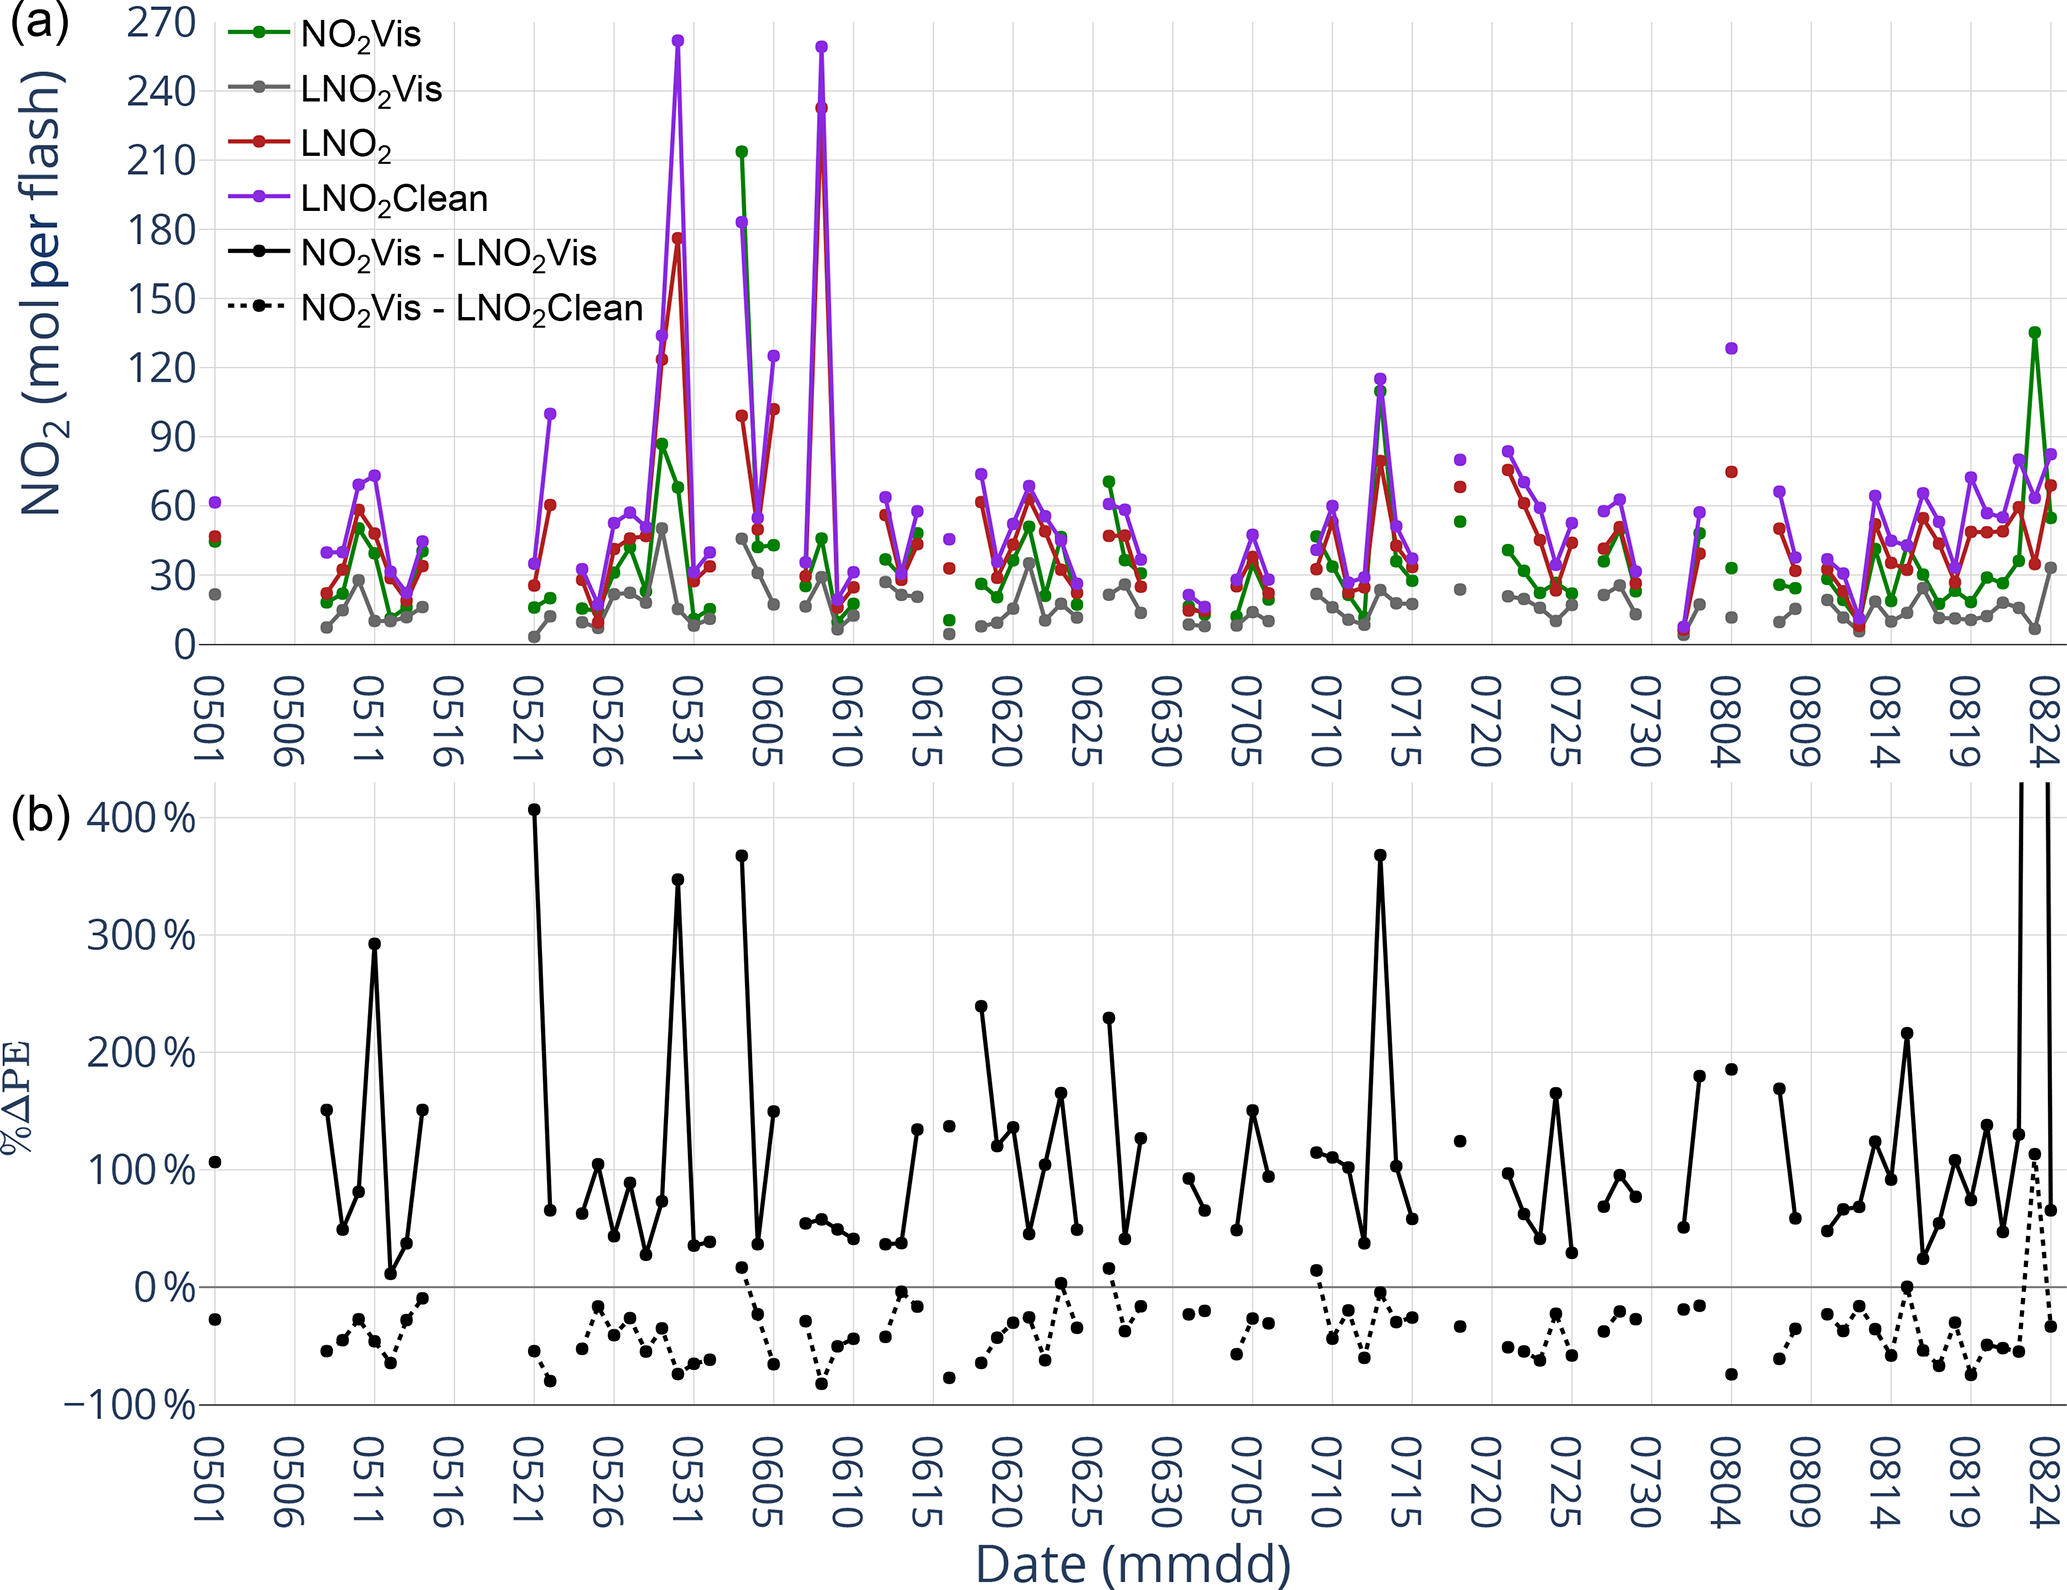
\includegraphics[width=12cm]{amt-2019-372-f03.png}
    \caption{\textbf{(a)} Time series of \chem{NO_2}Vis, L\chem{NO_2}Vis, L\chem{NO_2}, and L\chem{NO_2}Clean production per day over the CONUS for MJJA 2014 with CRF~$\geq 90$\,{\%} and a flash threshold of 2400 flashes per 2.4\,h.
    \textbf{(b)}~Time series of the percent differences between \chem{NO_2}Vis and L\chem{NO_2}Vis and the percent differences between \chem{NO_2}Vis and L\chem{NO_2}Clean with CRF~$\geq 90$\,{\%}.
    The value of the black dot on 23~August  (not shown) is 1958\,{\%}.}
    \label{fig:t_series}
\end{figure*}

Figure~\ref{fig:PE_linear} shows the linear regression for ENTLN data versus \chem{NO_2}Vis, L\chem{NO_2}Vis, L\chem{NO_2}, and L\chem{NO_2}Clean with the same criteria as shown in Fig.~\ref{fig:t_series}.
L\chem{NO_2}Clean PE (the largest slope) is $25.2 \pm 22.3$\,mol\,\chem{NO_2} per flash with a correlation of 0.25 and $2.3 \pm 2.1$\,mol\,\chem{NO_2} per stroke with a correlation of 0.22.
As shown in Fig.~\ref{fig:t_series}, positive percent differences between \chem{NO_2}Vis PE and L\chem{NO_2}Clean PE occur much less often than negative differences.
As a result, \chem{NO_2}Vis PE ($17.1 \pm 17.2$\,mol\,\chem{NO_2} per flash and $0.4 \pm 1.0$\,mol\,\chem{NO_2} per stroke) is smaller than L\chem{NO_2}Clean PE using the linear regression method.

In order to compare our result with that of \citet{Lapierre.2020}, we tried to remove the CP~$\leq 650$\,hPa, TL~$\geq 1000$, and ratio~$\geq 50$\,{\%} conditions from criteria.
But, our result based on daily summed \chem{NO_2}Vis values ($3.8 \pm 0.5$ mol per stroke) is still larger than the value of $1.6 \pm$ 0.1\,mol per stroke mentioned in \citet{Lapierre.2020}.
This may be caused by the different version of the BEHR algorithm, as \citet{Lapierre.2020} used BEHR v3.0A and our algorithm is based on BEHR v3.0B \citep{Laughner.2019}.
The input of S$_\chem{NO_2}$ in both versions is from the NASA standard product v3, and the major improvements of BEHR v3.0B are listed below.
\begin{enumerate}
\item The profile (v3.0B) closest to the OMI overpass time was selected instead of the last profile (v3.0A) before the OMI overpass.

\item The AMF uses a variable tropopause height as opposed to the fixed 200\,hPa tropopause.

\item The surface pressure is now calculated according to \citet{Zhou.2009}.
\end{enumerate}
The detailed log of changes is available at \url{https://github.com/CohenBerkeleyLab/BEHR-core/blob/master/Documentation/Changelog.txt} (last access: 20~March~2020).
Note that \citet{Lapierre.2020} used the monthly \chem{NO_2} profile. While the daily profile is used in our study and the interval of our outputs from WRF-Chem is 30\,min, which is more frequent than 1\,h in the BEHR daily product,
the AMF could be affected by different \chem{NO_2} profiles.
In view of these factors, we compare different methods based on our data to minimize these effects.

Meanwhile, L\chem{NO_2} PE ($18.7 \pm 18.1$\,mol per flash and $2.1\pm 1.8$\,mol per stroke) is between L\chem{NO_2}Clean PE and \chem{NO_2}Vis PE, which coincides with the daily results in Fig.~\ref{fig:t_series}.
Furthermore, the L\chem{NO_\mathit{x}} PE based on the linear regression of daily summed values,
the same method used in \citet{Pickering.2016},
is $114.8 \pm 18.2$\,mol per flash (or $17.8 \pm 2.9$\,mol per stroke), which is larger than 91\,mol per flash in \citet{Pickering.2016},
possibly due to the differences in geographic location, lightning data, and chemistry model.

%f4
\begin{figure*}[t]
    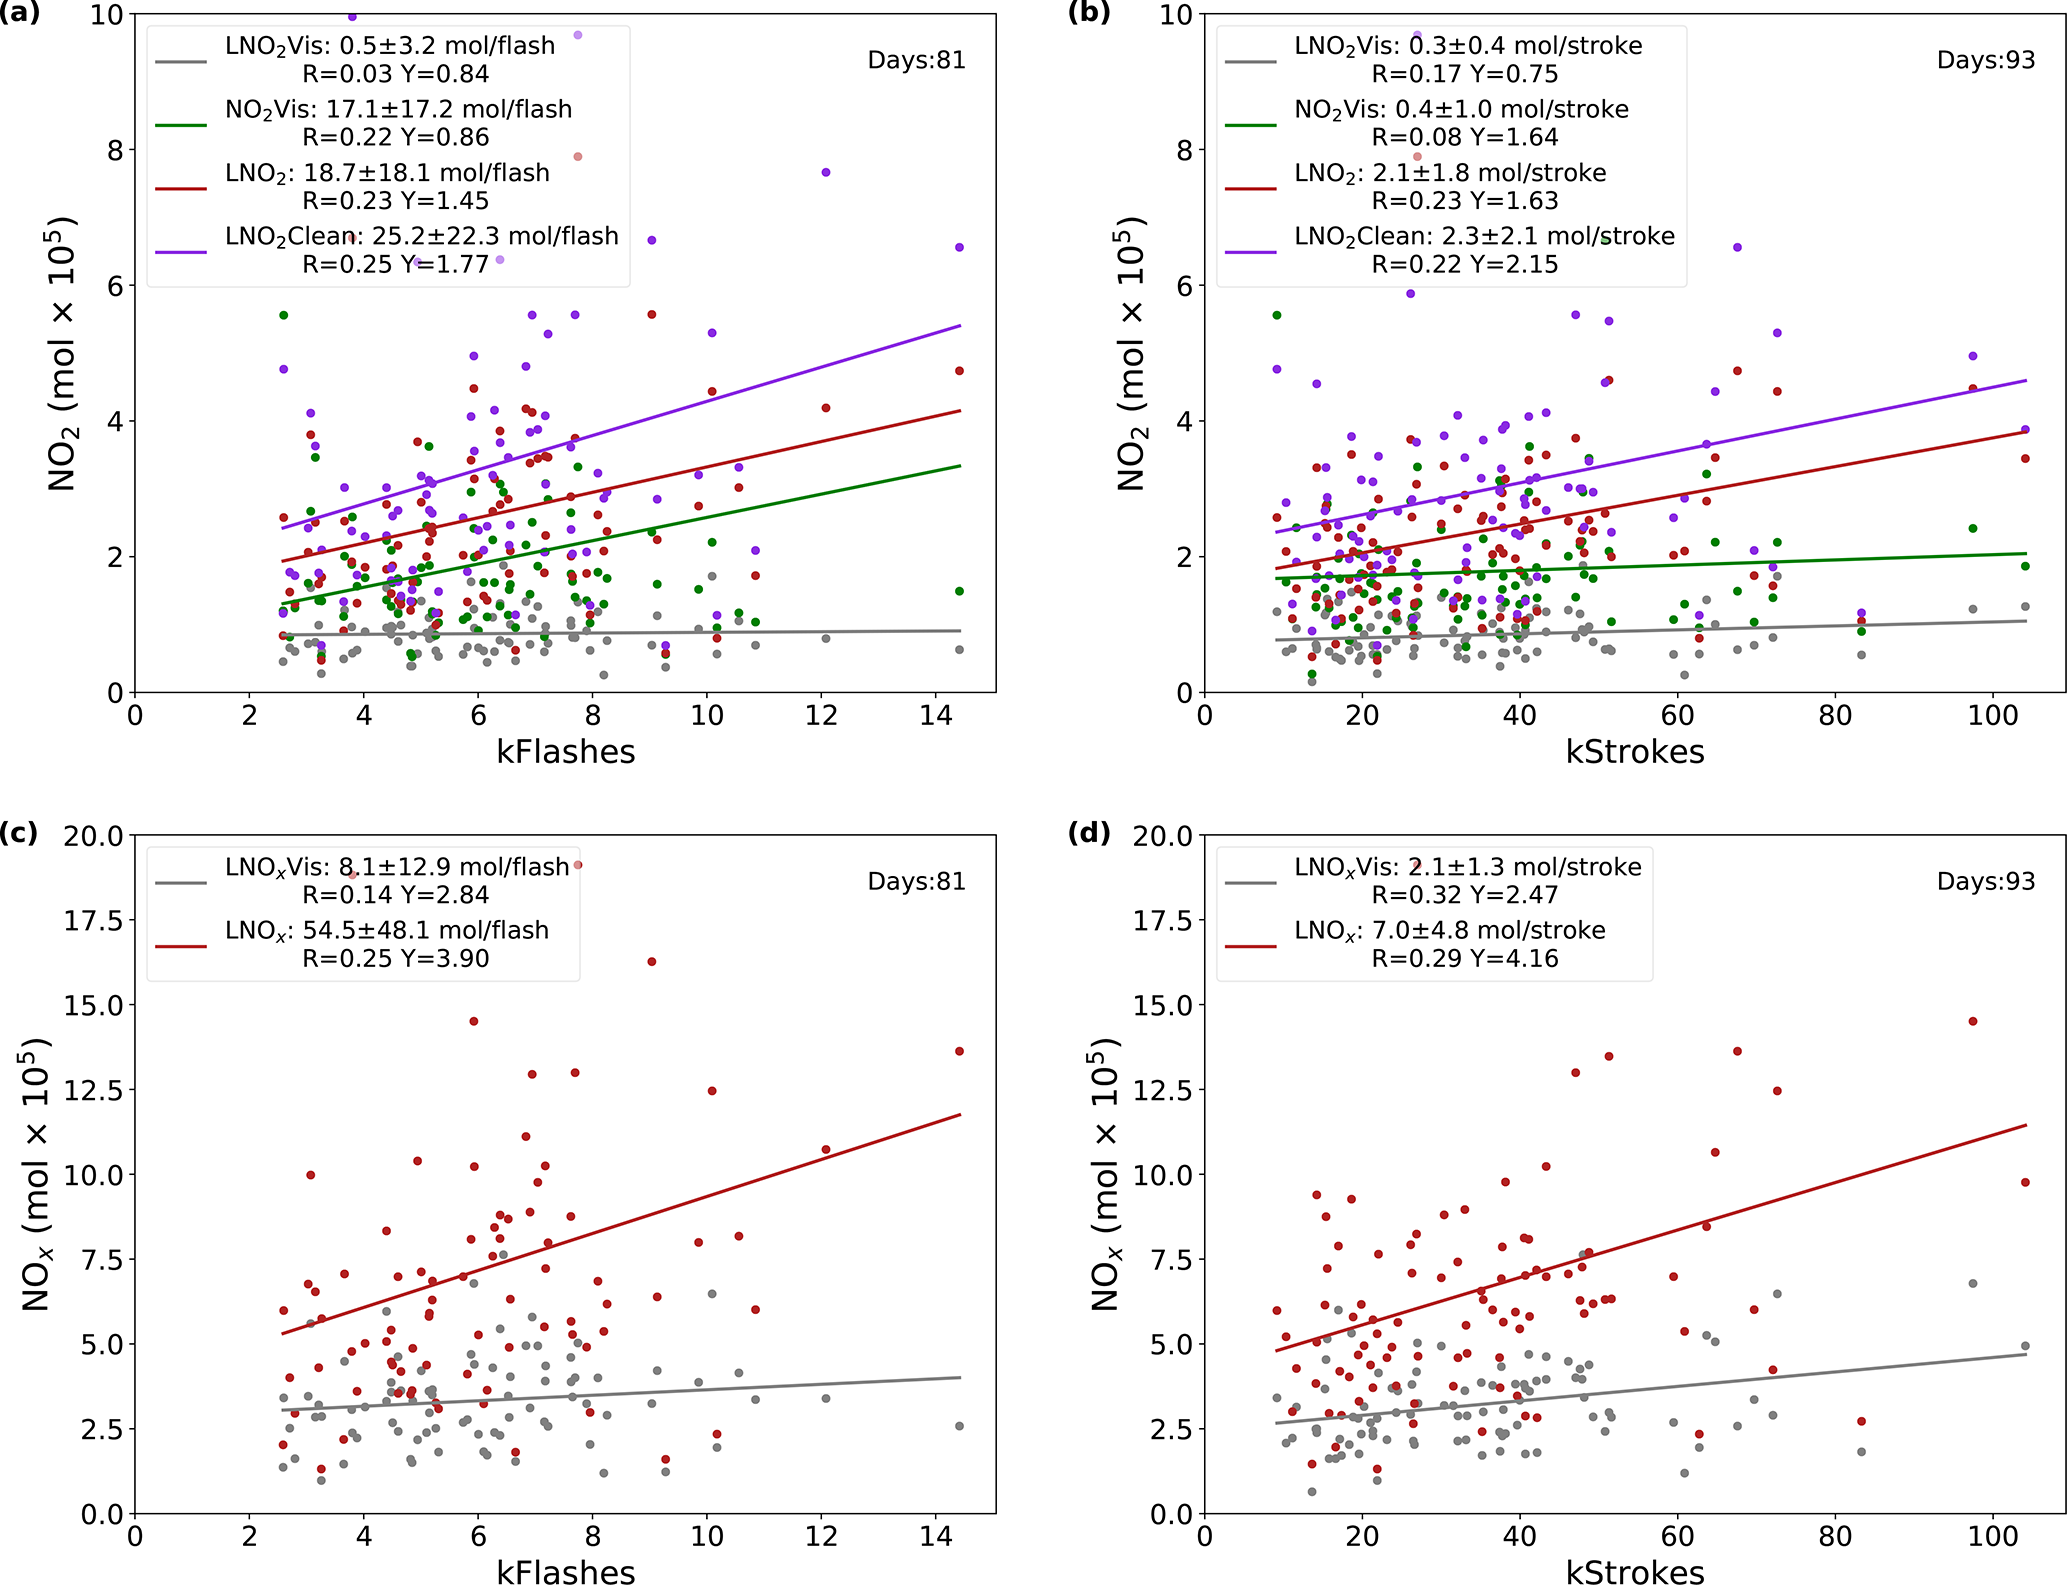
\includegraphics[width=15cm]{amt-2019-372-f04.png}
    \caption{\textbf{(a)} Daily \chem{NO_2}Vis, L\chem{NO_2}Vis, L\chem{NO_2}, and L\chem{NO_2}Clean versus ENTLN total flash data. \textbf{(b)}~Same as \textbf{(a)}~but for strokes. \textbf{(c)}~Daily L\chem{NO_\mathit{x}}Vis and L\chem{NO_\mathit{x}} versus total flashes. \textbf{(d)}~Same as \textbf{(c)}~but for strokes.}
    \label{fig:PE_linear}
\end{figure*}

The mean and standard deviation of L\chem{NO_2} PE under CRF~$\geq 90\,{\%}$ using the summation method is $46.2 \pm 35.1$\,mol per flash and $9.9 \pm 8.1$\,mol per stroke, while L\chem{NO_\mathit{x}} PE is $125.6 \pm 95.9$\,mol per flash and $26.7 \pm 21.6$\,mol per stroke (Fig.~\ref{fig:PE_sum}).
The L\chem{NO_2} PE and L\chem{NO_\mathit{x}} PE are both higher in the southeast US (denoted by the red box in Fig.~5, 25--37{\degree}\,N, 75--95{\degree}\,W), consistent with \citet{Lapierre.2020} and \citet{Bucsela.2019}.
Compared with Fig.~\ref{fig:t_series}, Fig.~\ref{fig:delta}a and~b present some large differences between \chem{NO_2}Vis PE and L\chem{NO_2}Vis PE, which are consistent with what we expect for polluted regions.
Meanwhile, the differences between L\chem{NO_2} PE and \chem{NO_2}Vis PE depend on background \chem{NO_2}, the strength of updraft, and the profile.
The negative differences are caused by background \chem{NO_2} carried by the updraft while parts of the below-cloud L\chem{NO_2} result in L\chem{NO_2} PE higher than \chem{NO_2}Vis PE (Fig.~\ref{fig:delta}c).
Figure~\ref{fig:delta}d shows that the ratio of L\chem{NO_2}Vis to L\chem{NO_2} ranges from 10\,{\%} to 80\,{\%}.
This may be caused by the height of the clouds and the profile of L\chem{NO_2}.
If the CP is near 300\,hPa, the ratio should be smaller because of the coverage of clouds.
While peaks of the L\chem{NO_2} profile are below the CP, the ratio would also be smaller.
Therefore, a better understanding of the L\chem{NO_2} profile and L\chem{NO_\mathit{x}} below clouds is required.

%f5
\begin{figure*}[t]
    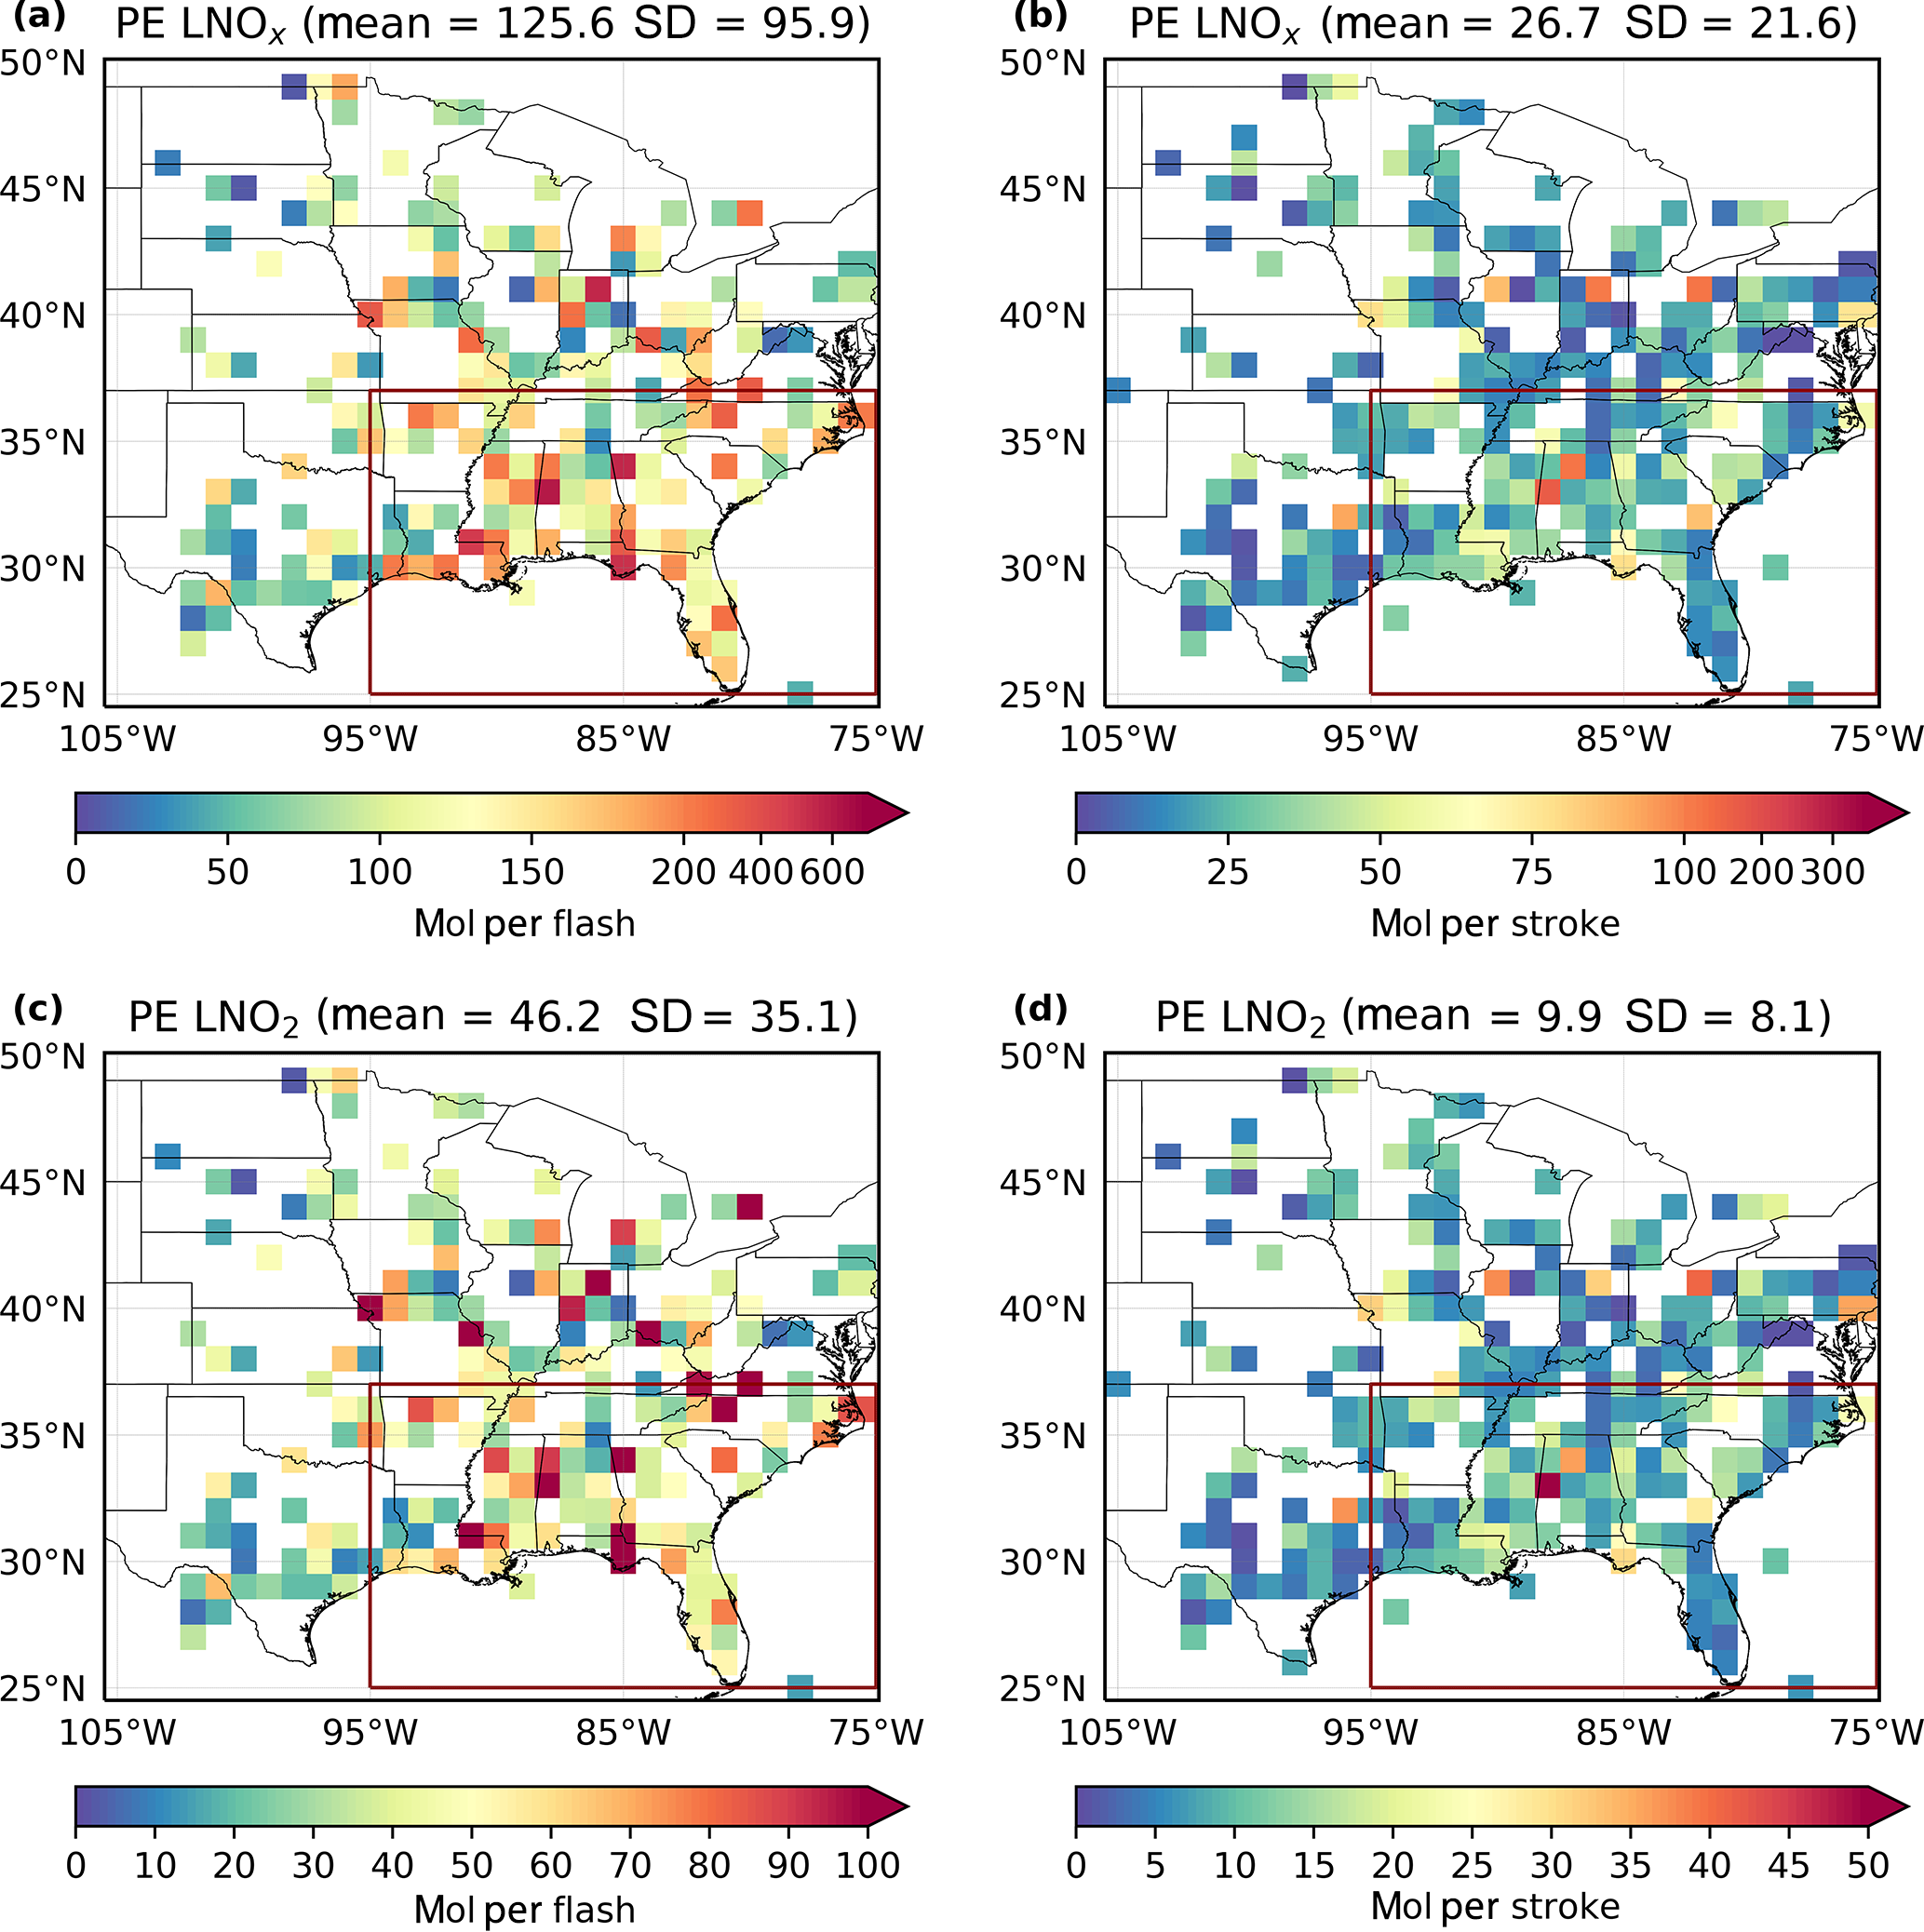
\includegraphics[width=13cm]{amt-2019-372-f05.png}
    \caption{\textbf{(a, c)}~Maps of $1{\degree}\times 1{\degree}$ gridded values of mean L\chem{NO_\mathit{x}}
        and L\chem{NO_2} production per flash with CRF~$\geq 90$\,{\%} for MJJA 2014.
        \textbf{(b, d)}~Same as \textbf{(a)}~and \textbf{(c)}~except for strokes.
        The southeastern US is denoted by the red box in panels~\textbf{(a)}--\textbf{(d)}.}
    \label{fig:PE_sum}
\end{figure*}

%f6
\begin{figure*}[t]
    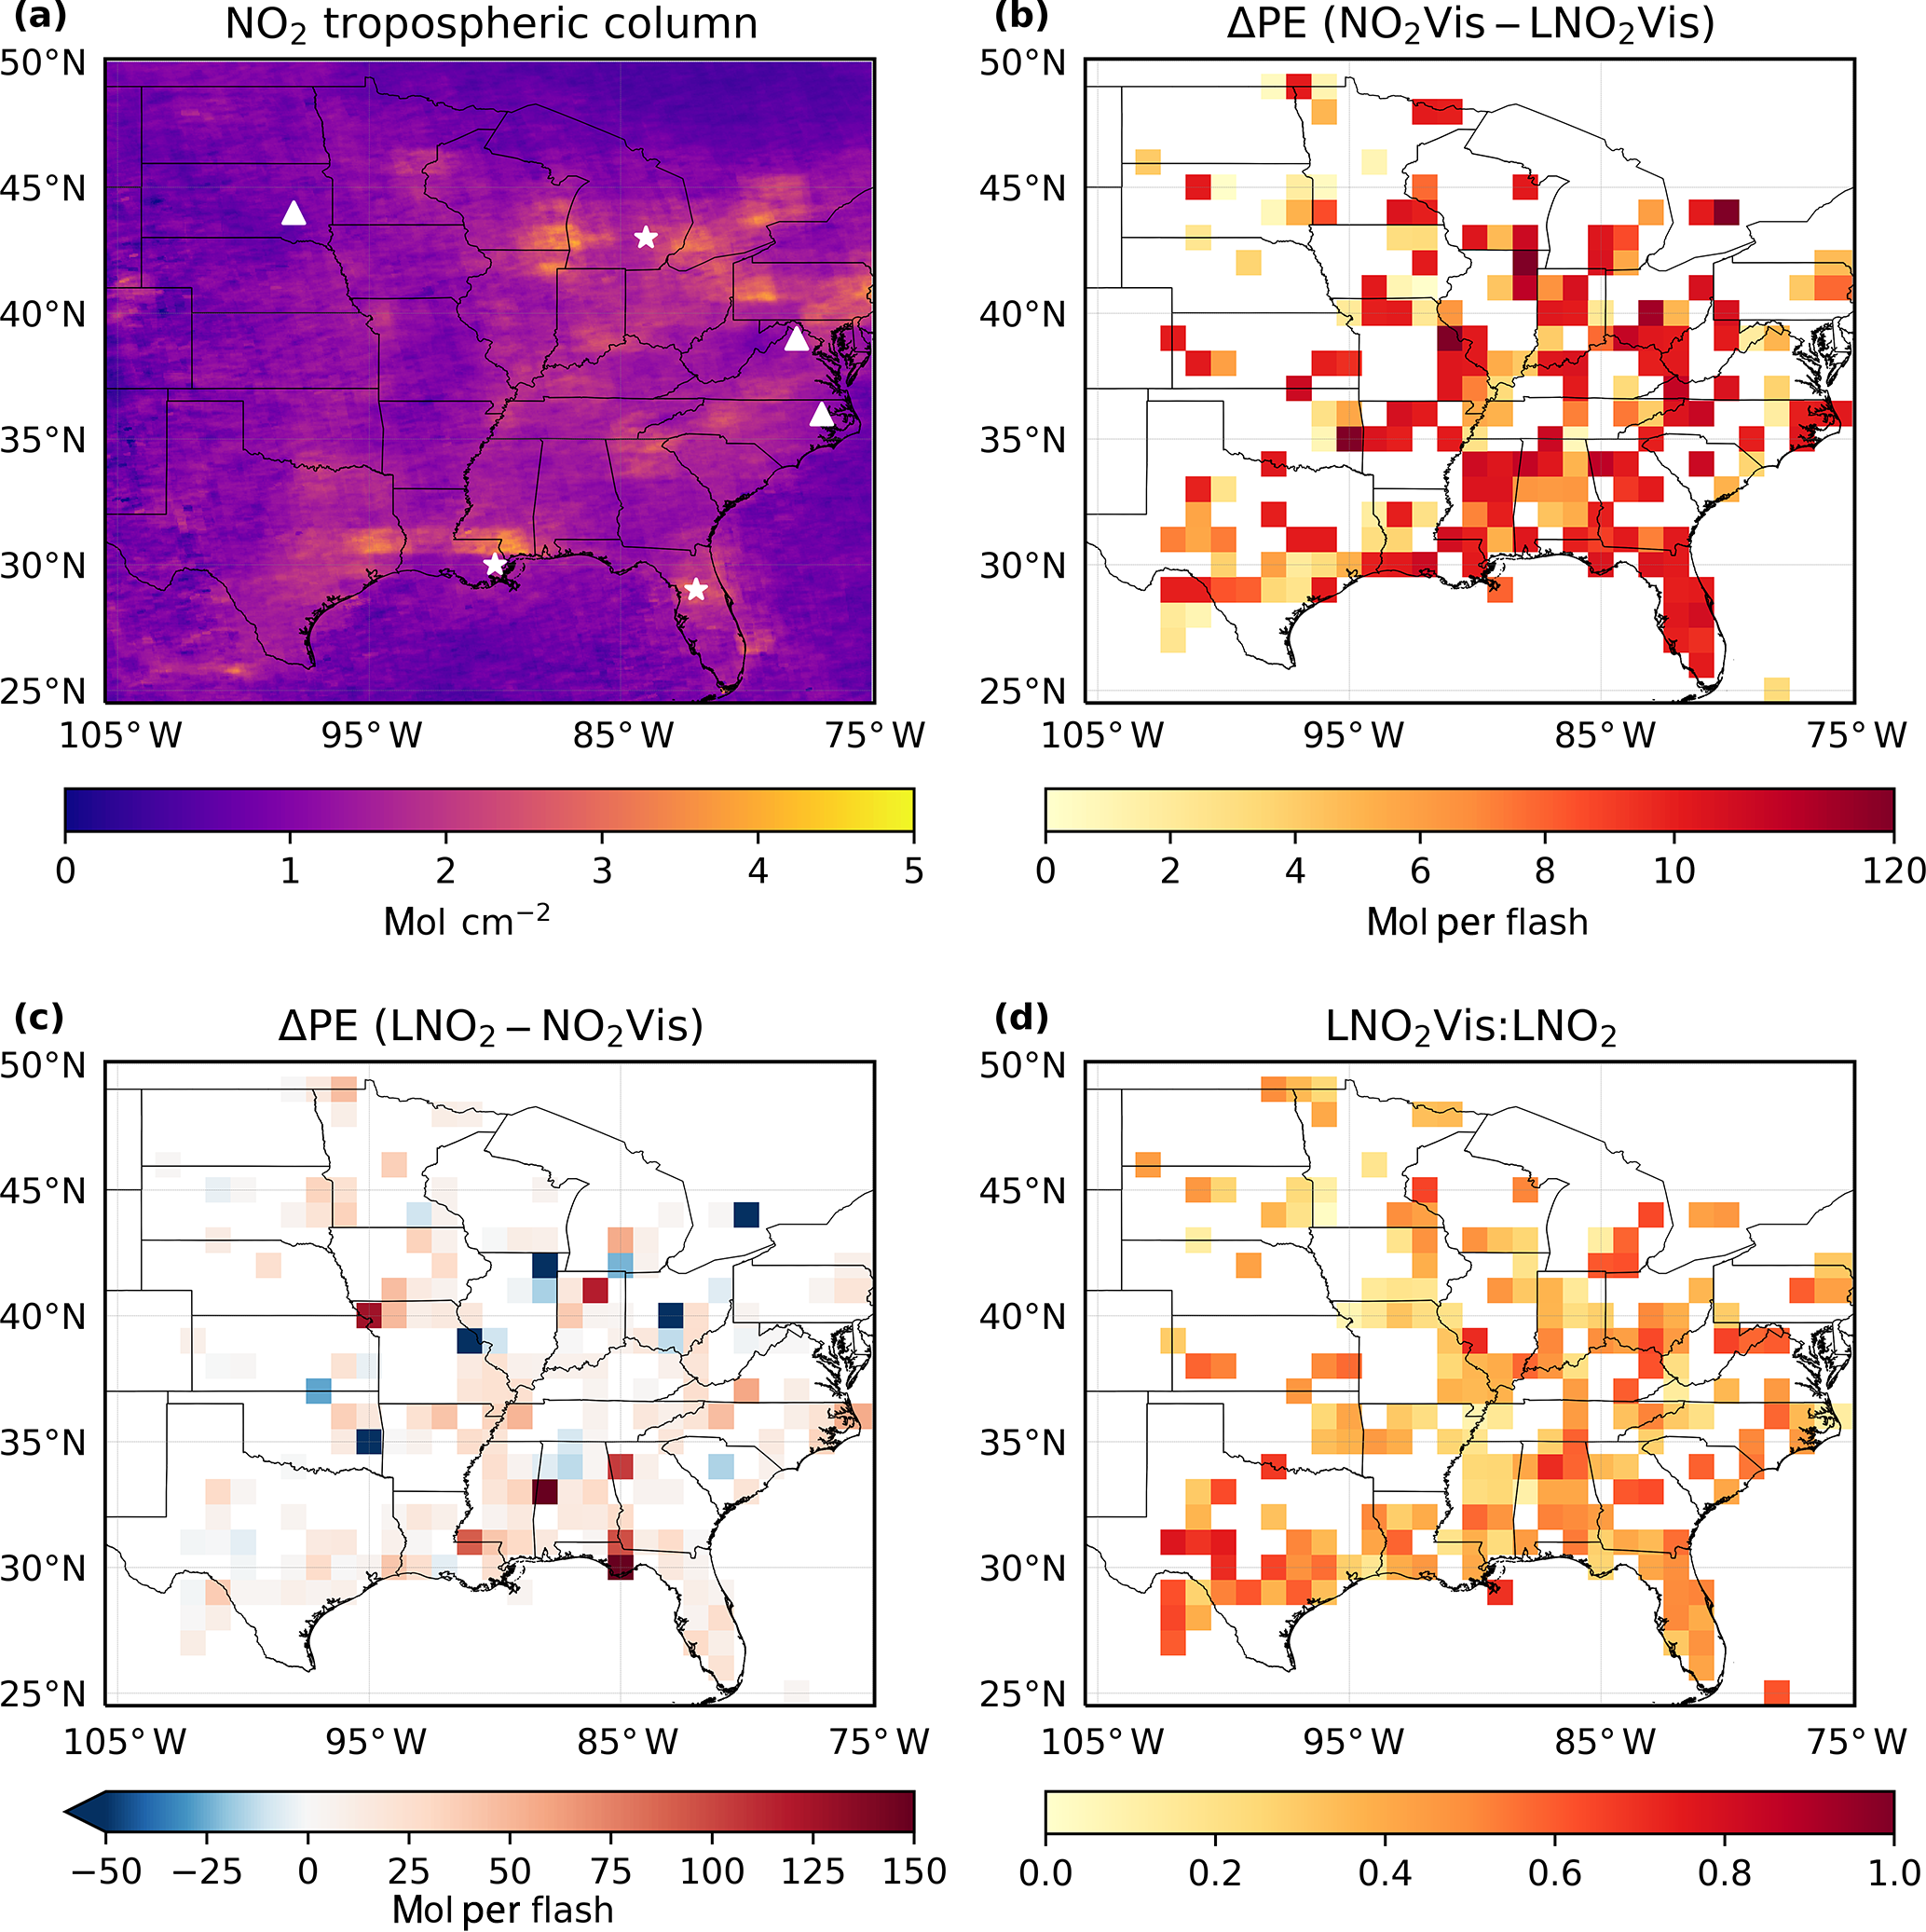
\includegraphics[width=12cm]{amt-2019-372-f06.png}
    \caption{\textbf{(a)} Mean (MJJA 2014) \chem{NO_2} tropospheric column.
        Polluted cities are denoted by stars (Lansing, New Orleans, and Orlando) while clean cities are denoted by triangles (Huron, Charles Town, and Tarboro).
        \textbf{(b)}~The differences of the estimated mean production efficiency between \chem{NO_2}Vis and L\chem{NO_2}Vis with CRF~$\geq 90$\,{\%}.
        \textbf{(c)}~The same differences as \textbf{(b)}~but between L\chem{NO_2} and \chem{NO_2}Vis.
        \textbf{(d)}The ratio of L\chem{NO_2}Vis to L\chem{NO_2}.}
    \label{fig:delta}
\end{figure*}

\subsection{Effects of tropospheric background on L\chem{NO_\mathit{x}} production}
\label{section:Effectsofbackground}

With respect to the L\chem{NO_2} production, the patterns in Fig.~\ref{fig:delta} indicate the improvement of our approach is different in polluted and clean regions.
To simplify the quantification, we select six grids with similar \chem{NO_2} profiles ($\sim 100$\,pptv) above the cloud with CRF~$= 100$\,{\%}.
These grid boxes contain the polluted and clean cities denoted by stars and triangles in Fig.~\ref{fig:delta}a, respectively.
Then, the differences between AMFs are dependent on fewer parameters.
\begin{gather} \label{AMFLNO2_crf100}
\mathrm{AMF}_{\chem{LNO_2}} = \frac{\int_{p_\mathrm{cloud}}^{p_\mathrm{tp}} w_\mathrm{cloudy}(p) \chem{NO_2}(p) \: \mathrm{d}p}{\int_{p_\mathrm{surf}}^{p_\mathrm{tp}} \chem{LNO_2}(p) \: \mathrm{d}p}
\\
 \label{AMFNO2Vis_crf100}
\mathrm{AMF}_{\chem{NO_2}\mathrm{Vis}} = \frac{\int_{p_\mathrm{cloud}}^{p_\mathrm{tp}} w_\mathrm{cloudy}(p) \chem{NO_2}(p) \: \mathrm{d}p}{\int_{p_\mathrm{cld}}^{p_\mathrm{tp}} \chem{NO_2}(p) \: \mathrm{d}p}
\\ \label{AMFLNO2Clean_crf100}
\mathrm{AMF}_{\chem{LNO_2}\mathrm{Clean}} = \frac{\int_{p_\mathrm{cloud}}^{p_\mathrm{tp}} w_\mathrm{cloudy}(p) \chem{LNO_2}(p) \: \mathrm{d}p}{\int_{p_\mathrm{surf}}^{p_\mathrm{tp}} \chem{LNO_2}(p) \: \mathrm{d}p}
\end{gather}
Figure~\ref{fig:backgroundcomparisons} compares the mean profiles of \chem{NO_2}, background \chem{NO_2} and background \chem{NO_2} ratio in polluted and clean grids.
Generally, the profiles of the ratio of background \chem{NO_2} to total \chem{NO_2} are C shaped because UT L\chem{NO_2} concentrations are higher than UT background \chem{NO_2} concentrations.
However, the ratio profile in Fig.~\ref{fig:backgroundcomparisons}e has one peak between the cloud pressure and tropopause as background \chem{NO_2} increases and L\chem{NO_2} decreases.
Besides, the percentage of UT background \chem{NO_2} in polluted regions is steady and higher than that in clean regions.

Table~\ref{table:productioncomparisons} presents the relative changes among three methods in six cities.
The difference between AMF$_{\chem{LNO_2}}$ (Eq.~\ref{AMFLNO2_crf100}) and AMF$_{\chem{LNO_2}\mathrm{Clean}}$ (Eq.~\ref{AMFLNO2Clean_crf100}) is the numerator: $\int_{p_\mathrm{cloud}}^{p_\mathrm{tp}} w_\mathrm{cloudy}(p) \chem{NO_2}(p) \: \mathrm{d}p$ and $\int_{p_\mathrm{cloud}}^{p_\mathrm{tp}} w_\mathrm{ cloudy}(p) \chem{LNO_2}(p) \: \mathrm{d}p$.
When the ratio of L\chem{NO_2} is higher or the region is cleaner, the relative difference is smaller (e.g. 5.0\,{\%}--12.0\,{\%}, Fig.~\ref{fig:backgroundcomparisons}d--f).
The largest relative difference (46.3\,{\%}) occurs when the ratio of background \chem{NO_2} is continuously high in the UT (Fig.~\ref{fig:backgroundcomparisons}c).
As a result, our approach is less sensitive to background \chem{NO_2} and more suitable for convective cases over polluted locations.
In contrast, production estimated by our method is larger than that based on \chem{NO_2}Vis due to the L\chem{NO_2} below the cloud.
When the cloud is higher, in particular the peak of the LNO profile is lower than the cloud (Fig.~\ref{fig:backgroundcomparisons}b). The relative difference is larger (121.2\,{\%}) because more L\chem{NO_2} can not be included in the \chem{NO_2}Vis, which has been discussed in Sect.~\ref{section:Comparison}.
The relative change between AMF$_{\chem{LNO_2}\mathrm{Clean}}$ (Eq.~\ref{AMFLNO2Clean_crf100}) and AMF$_{\chem{NO_2}\mathrm{Vis}}$ (Eq.~\ref{AMFNO2Vis_crf100}) depends on $\int_{p_\mathrm{cloud}}^{p_\mathrm{tp}} w_\mathrm{cloudy}(p) \chem{LNO_2}(p) \: \mathrm{d}p / \int_{p_\mathrm{surf}}^{p_\mathrm{tp}} w_\mathrm{cloudy}(p) \chem{LNO_2}(p) \: \mathrm{d}p$, which is also affected by cloud, not the background \chem{NO_2}.
The largest relative change (153.8\,{\%}) occurs at New Orleans, which has the lowest cloud pressure and consequently the smallest visible column.

%f7
\begin{figure*}[t]
    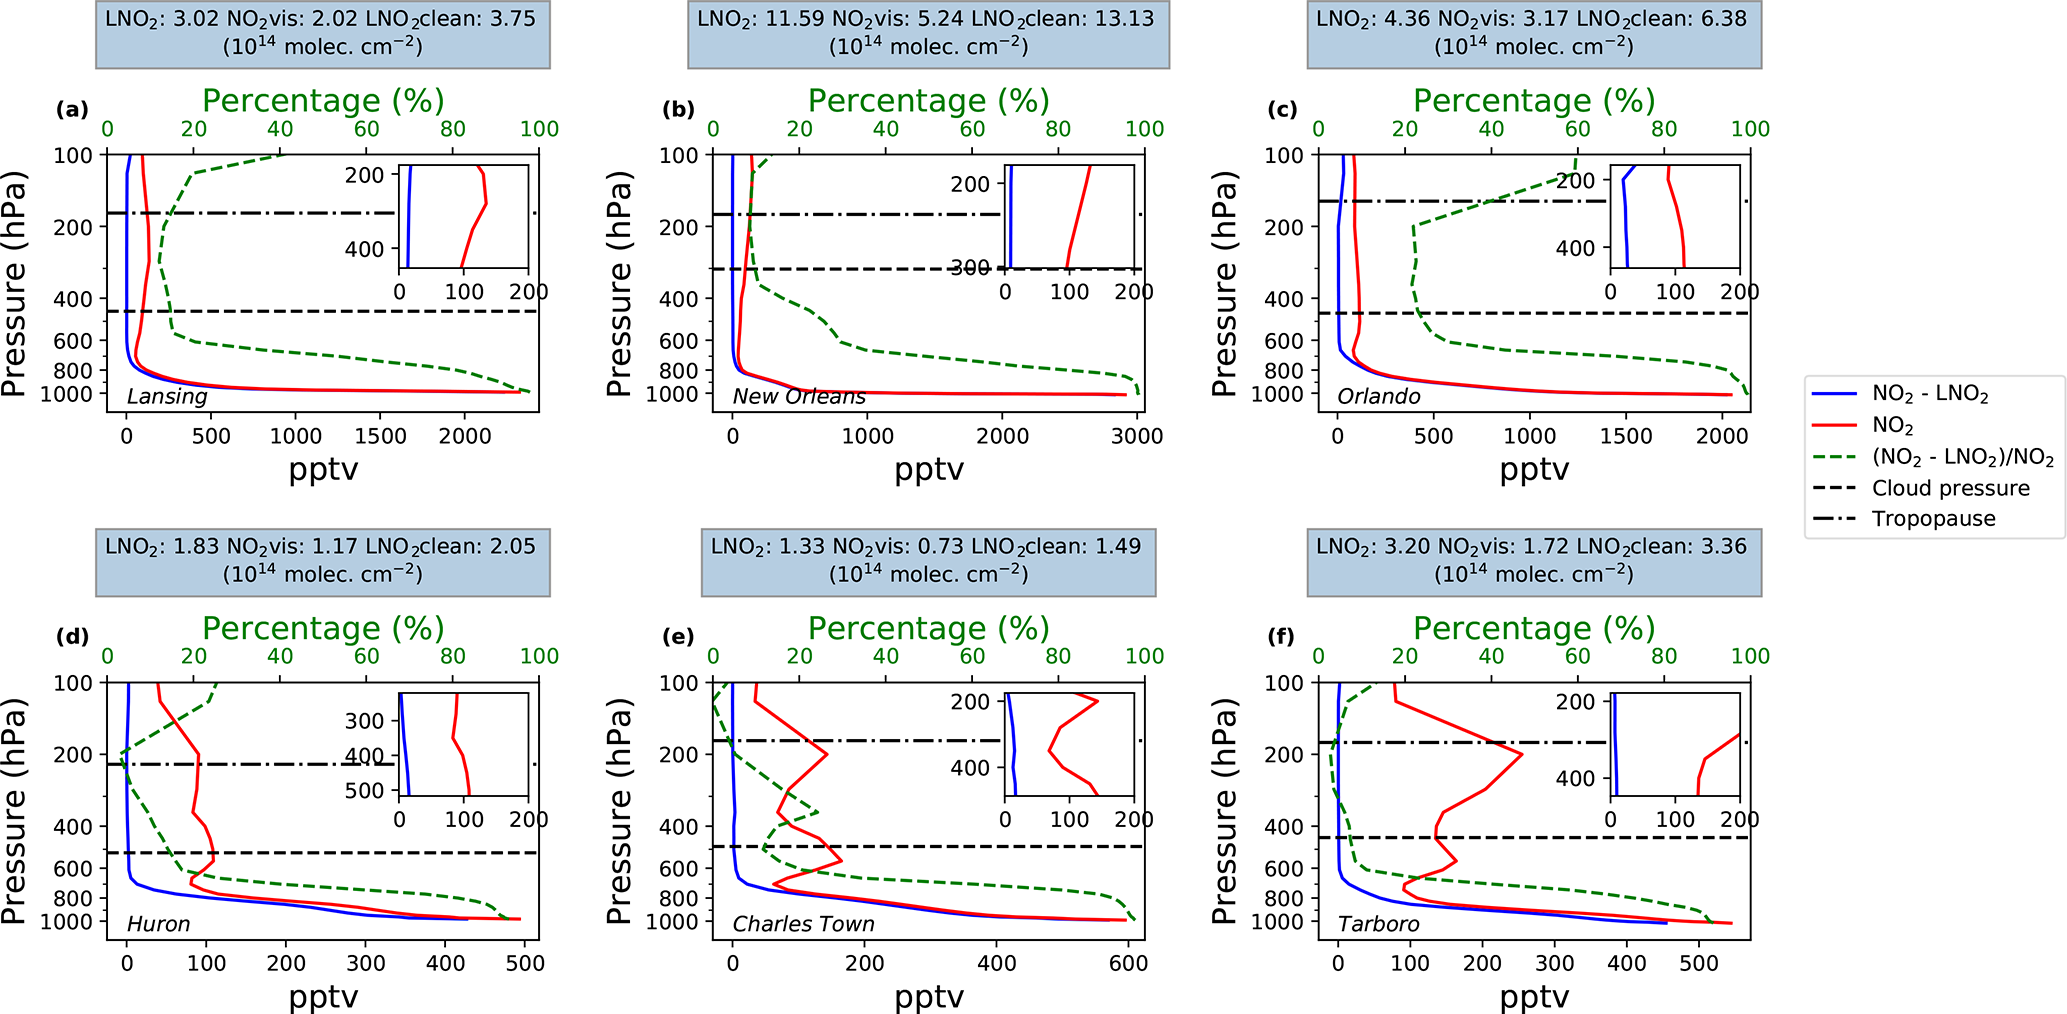
\includegraphics[width=17.5cm]{amt-2019-372-f07.png}
    \caption{Comparisons of mean WRF-Chem \chem{NO_2} and background \chem{NO_2} profiles in six grids with CRF~$\geq 100$\,{\%} on specific days during MJJA 2014.
    The~\textbf{(a)}, \textbf{(b)}, and \textbf{(c)}~data are selected from polluted regions (stars in Fig.~\ref{fig:delta}a) while the~\textbf{(d)}, \textbf{(e)}, and \textbf{(f)}~data are from clean regions (triangles in Fig.~\ref{fig:delta}a).
    The green dashed lines are the mean ratio profiles of background \chem{NO_2} to total \chem{NO_2}.
    The zoomed figures show the profiles from the cloud pressure to the tropopause.
    The titles present the mean productions based on three different methods mentioned in Sect.~\ref{section:AMF}.}
    \label{fig:backgroundcomparisons}
\end{figure*}

%f8
\begin{figure*}[t]
    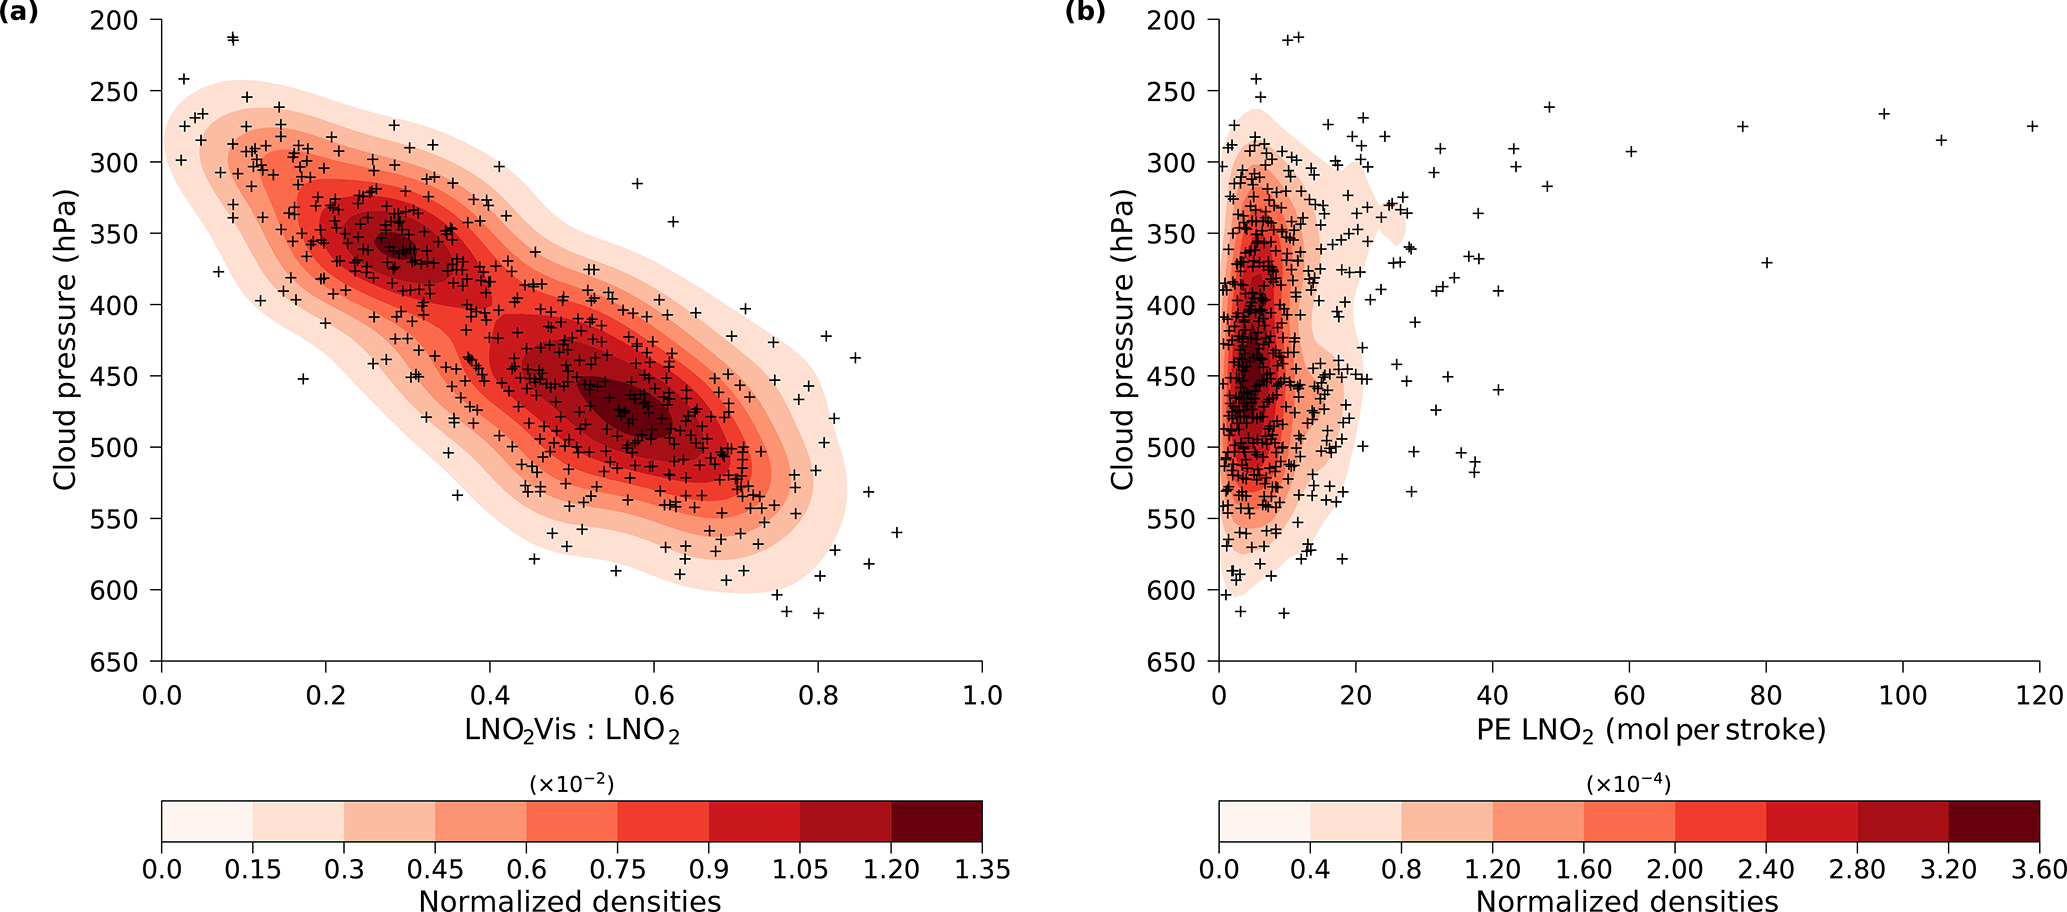
\includegraphics[width=15cm]{amt-2019-372-f08.png}
    \caption{Kernel density estimation of the \textbf{(a)}~daily ratio of L\chem{NO_2}Vis to L\chem{NO_2} and \textbf{(b)}~daily L\chem{NO_2} production efficiency versus the daily cloud pressure measured by OMI with CRF~$\geq 90$\,{\%} for MJJA 2014.
    The kernel density estimation was generated by kdeplot in the Python package named seaborn.}
    \label{fig:CP_ratio_LNO2}
\end{figure*}



%f9
\begin{figure*}[t]
    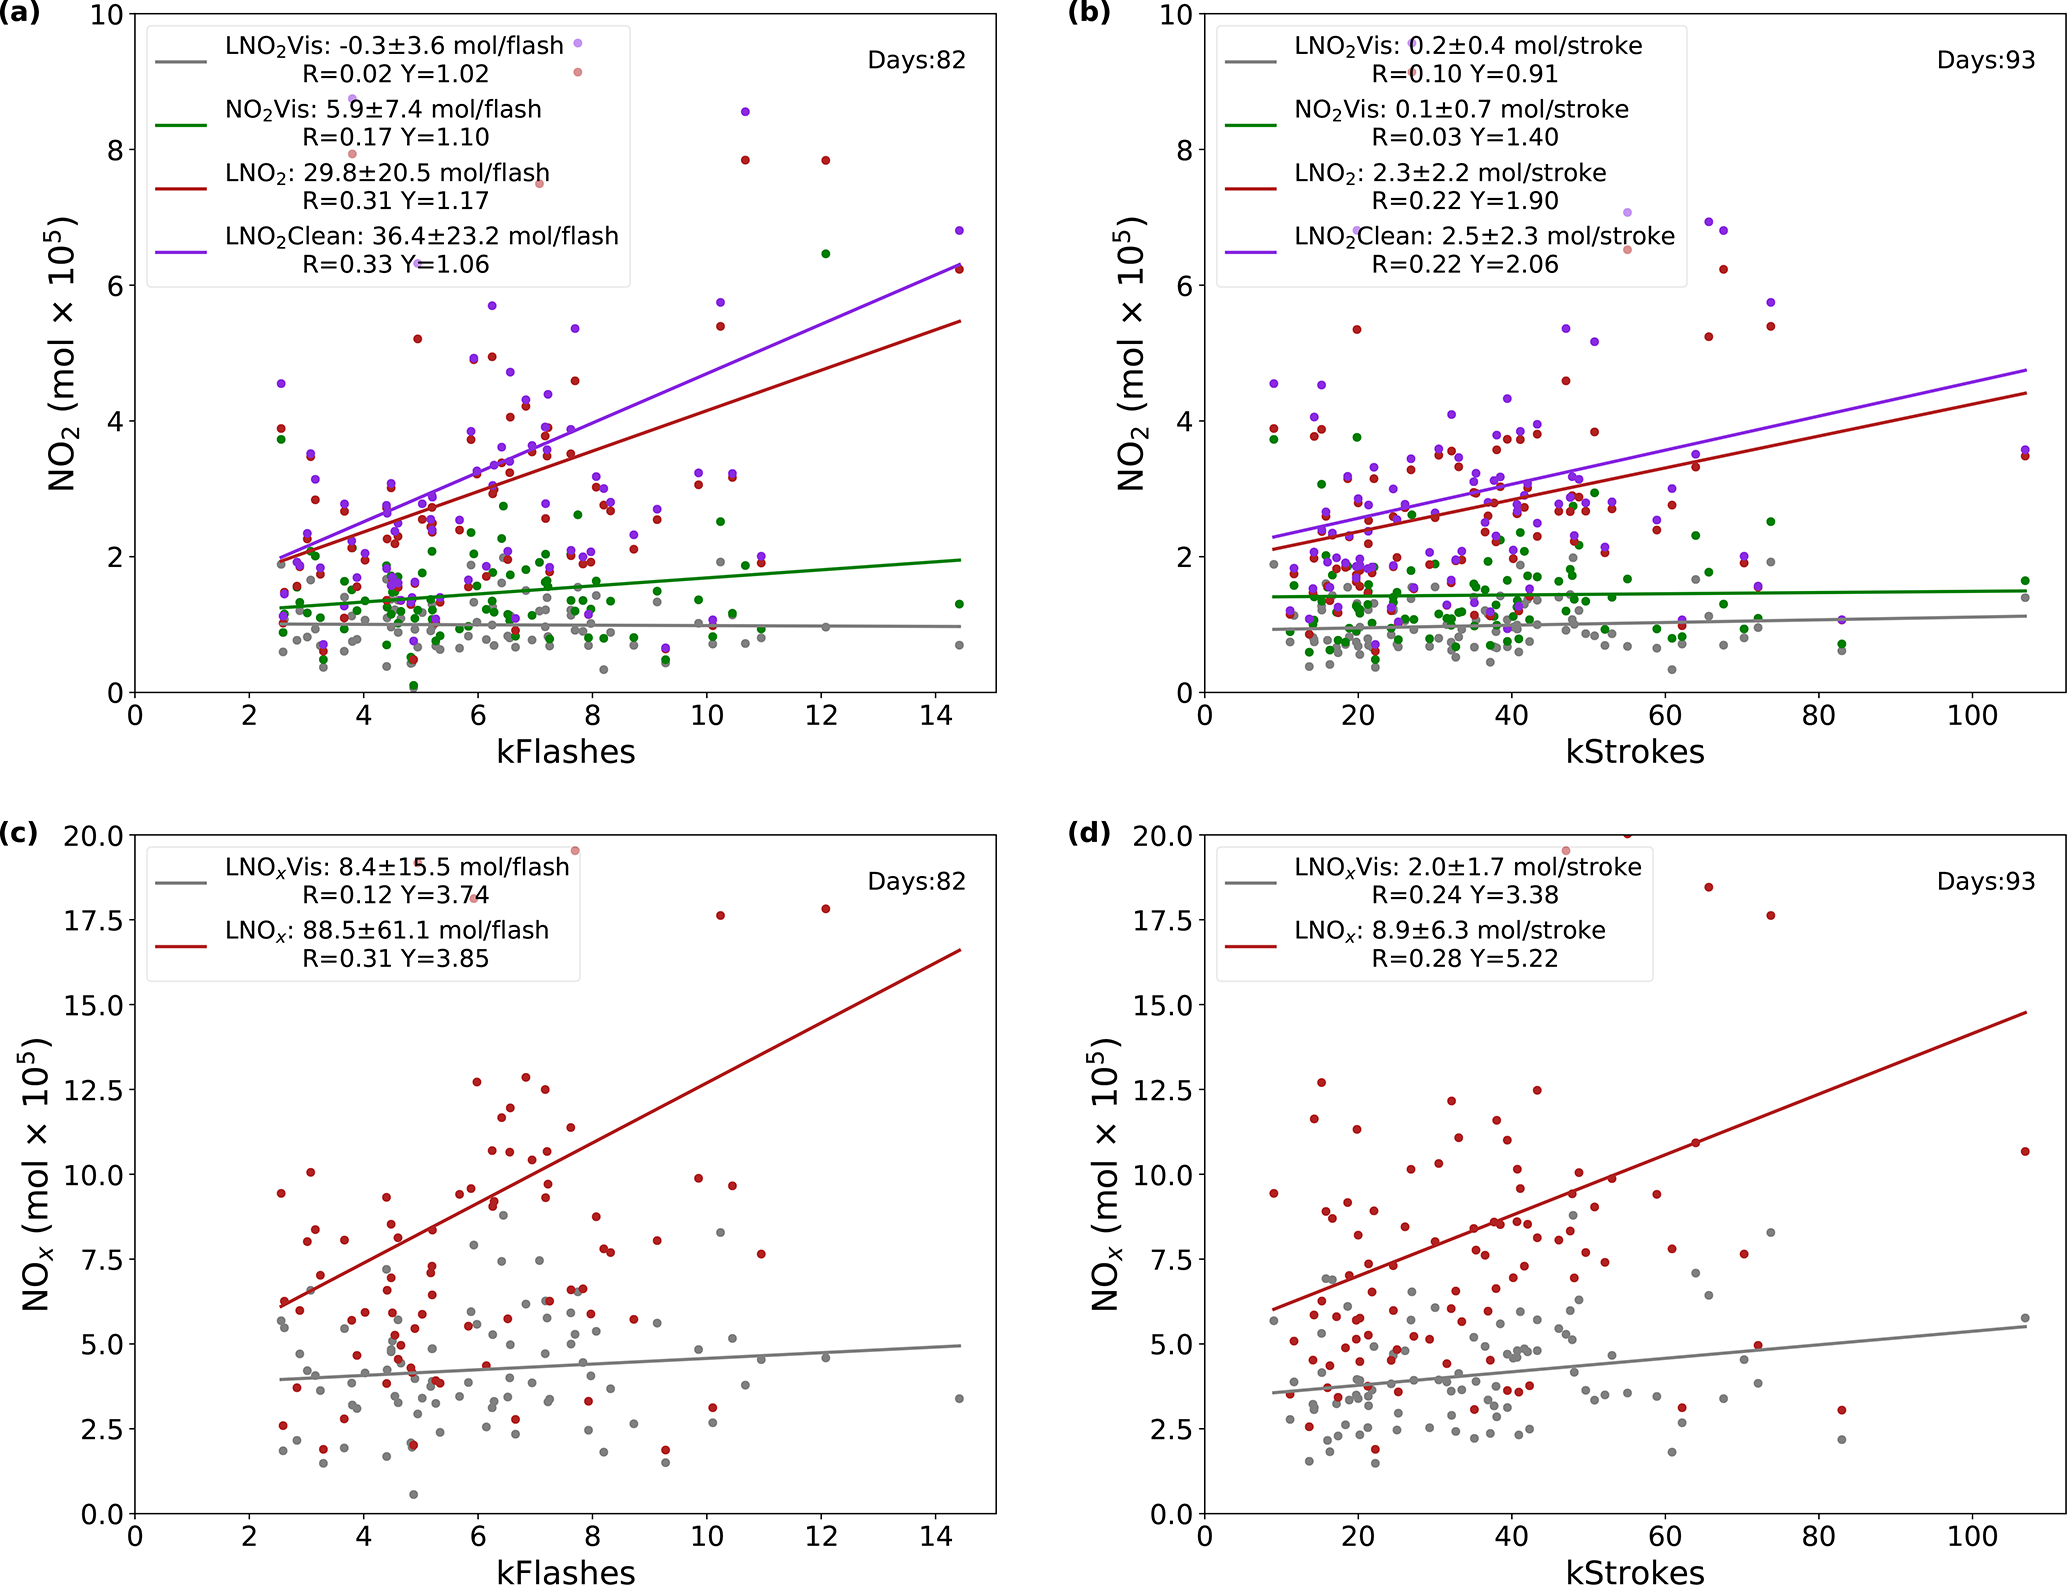
\includegraphics[width=15cm]{amt-2019-372-f09.png}
    \caption{Same as Fig.~\ref{fig:PE_linear} except for the $2\times500$\,mol\,NO per flash configuration.}
    \label{fig:PE_linear_2x500}
\end{figure*}
\subsection{Effects of cloud and L\chem{NO_\mathit{x}} parameterization on L\chem{NO_\mathit{x}} production} \label{section:Effectsofcloud}

Figure~\ref{fig:CP_ratio_LNO2}a presents the daily distribution of CP and the ratio of L\chem{NO_2}Vis to L\chem{NO_2} during MJJA 2014 with the criteria defined in Sect.~\ref{section:Criteria} under CRF~$\geq 90$\,{\%}.
Since the ratio of L\chem{NO_2}Vis to L\chem{NO_2} decreases from 0.8 to 0.2 as the cloud pressure decreases from 600 to 300\,hPa, \chem{NO_2}Vis PE is smaller than L\chem{NO_2} PE in relatively clean areas as shown in Fig.~\ref{fig:PE_linear}.
Apart from L\chem{NO_2}Vis, the L\chem{NO_2} PE is also affected by CP.
For L\chem{NO_2} PEs larger than 30\,mol per stroke, the CPs are all smaller than 550\,hPa (Fig.~\ref{fig:CP_ratio_LNO2}b).
However, smaller L\chem{NO_2} PEs ($< 30$\,mol per stroke) occur on all levels between 650 and 200\,hPa.
Because of the limited number of large L\chem{NO_2} PEs and lightning data, we cannot derive the relationship between L\chem{NO_2} PE and cloud pressure or other lightning properties at this stage.
Because the CP only represents the development of clouds, the vertical structure of flashes can not be derived from the CP values only.
As discussed in several previous studies, the flash channel length varies and depends on the environmental conditions \citep{Carey.2016,Mecikalski.2017,Fuchs.2018}.
\citet{Davis.2019} compared two kinds of flash: normal flashes and anomalous flashes.
Because updrafts are stronger and flash rates are higher in anomalous storms, UT L\chem{NO_\mathit{x}} concentrations are larger in anomalous than normal polarity storms.
In general, normal flashes are coupled with an upper-level positive charge region and a midlevel negative charge region, while anomalous flashes are opposite \citep{Williams.1989}.
It is not straightforward to estimate the error resulting from the vertical distribution of L\chem{NO_\mathit{x}}.
There are mainly two methods of distributing L\chem{NO_\mathit{x}} in models: L\chem{NO_\mathit{x}} profiles (postconvection) in which L\chem{NO_\mathit{x}} has already been redistributed by convective transport and L\chem{NO_\mathit{x}} production profiles (preconvection) made before the redistribution of convective transport \citep{Allen.2012,Luo.2017}.
However, given the similarity of results compared to other L\chem{NO_\mathit{x}} studies, we believe that our $1{\degree}\times 1{\degree}$ results based on postconvective L\chem{NO_\mathit{x}} profiles are sufficient for estimating average L\chem{NO_\mathit{x}} production.
%t4
\begin{table*}[t]
  \caption{The percent changes in the estimated production when using different methods based on the same a priori profiles.}
  \begin{tabular}{llrrr}
    \tophline
   & {City$^*$} & {(L\chem{NO_2}Clean -- L\chem{NO_2})/L\chem{NO_2}} & {(L\chem{NO_2} -- TropVis)/TropVis} & {(L\chem{NO_2}Clean-TropVis)/TropVis} \\
    \middlehline
    \multirow{3}{*}{{Polluted}} & Lansing          & 24.2\,{\%}  & 49.5\,{\%}   & 85.6\,{\%}   \\
                                       & New Orleans      & 13.3\,{\%}  & 121.2\,{\%}  & 153.8\,{\%}  \\
                                       & Orlando          & 46.3\,{\%}  & 37.5\,{\%}   & 101.3\,{\%}  \\
    \middlehline
    \multirow{3}{*}{{Clean}}    & Huron            & 12.0\,{\%}  & 56.4\,{\%}   & 75.2\,{\%}   \\
                                       & Charles Town     & 12.0\,{\%}  & 82.2\,{\%}   & 104.1\,{\%}  \\
                                       & Tarboro          & 5.0\,{\%}   & 86.0\,{\%}   & 95.3\,{\%}   \\
    \bottomhline
  \end{tabular}
  \belowtable{$^*$~Locations are denoted in Fig.~\ref{fig:delta}a.}
  \label{table:productioncomparisons}
\end{table*}

The LNO production settings in WRF-Chem varied in different studies.
\citet{Zhao.2009} set a \chem{NO_\mathit{x}} production rate of 250\,mol\,NO per flash in a regional-scale model, while \citet{Bela.2016} chose 330\,mol\,NO per flash used by \citet{Barth.2012}.
\citet{Wang.2015} assumed approximately 500\,mol\,NO per flash, which was derived by a cloud-scale chemical transport model and in-cloud aircraft observations \citep{Ott.2010}.
To illustrate the impact of L\chem{NO_\mathit{x}} parameterization on L\chem{NO_\mathit{x}} estimation, we apply another WRF-Chem \chem{NO_2} profile setting ($2\times$~base flash rate, 500\,mol\,NO per flash, hereinafter referred to as ``$2\times500$\,mol\,NO per flash'') to a priori profiles and evaluate the changes in AMF$_{\chem{LNO_2}}$, AMF$_{\chem{LNO_\mathit{x}}}$, L\chem{NO_2} PE, and L\chem{NO_\mathit{x}} PE.
For the linear regression method (Fig.~\ref{fig:PE_linear_2x500}), L\chem{NO_2} PE is $29.8 \pm 20.5$\,mol per flash, which is 59.4\,{\%} larger than the basic one ($18.7 \pm 18.1$\,mol per flash).
Meanwhile, L\chem{NO_\mathit{x}} PE (increasing from $54.5 \pm 48.1$\,mol per flash to $88.5 \pm 61.1$\,mol per flash) also depends on the configuration of LNO production in WRF-Chem.
The comparison between Figs.~\ref{fig:PE_linear} and~\ref{fig:PE_linear_2x500} shows that L\chem{NO_2}Clean PE and L\chem{NO_2} PE are more similar while L\chem{NO_2} PE and \chem{NO_2}Vis PE present the same tendency.
It remains unclear as to whether the NO--\chem{NO_2}--\chem{O_3} cycle or other L\chem{NO_\mathit{x}} reservoirs account for the increment of L\chem{NO_\mathit{x}} PE.
This would need detailed source analysis in WRF-Chem and is beyond the scope of this study.

Figure~\ref{fig:simulation_diff} shows the average percentage changes in AMF$_{\chem{LNO_2}}$, AMF$_{\chem{LNO_\mathit{x}}}$, L\chem{NO_2}, and L\chem{NO_\mathit{x}} between retrievals using profiles based on $1\times200$ and $2\times500$\,mol\,NO per flash.
These results were obtained by averaging data over MJJA 2014 based on the method described in Sect.~\ref{section:Conditions} with the criterion of CRF~$\geq 90\,{\%}$.
The effects on L\chem{NO_2} and L\chem{NO_\mathit{x}} retrieval from increasing LNO profile values show mostly the same tendency: smaller AMF$_{\chem{LNO_2}}$ and AMF$_{\chem{LNO_\mathit{x}}}$ lead to larger L\chem{NO_2} and L\chem{NO_\mathit{x}}, but the changes are regionally dependent.
This is caused by the nonlinear calculation of AMF$_{\chem{LNO_2}}$ and AMF$_{\chem{LNO_\mathit{x}}}$.
As the contribution of L\chem{NO_2} increases, both the numerator and denominator of Eq.~(\ref{AMFLNOx}) increase.
Note that the L\chem{NO_2} accounts for a fraction of \chem{NO_2} above the clouds. The magnitude of an increasing denominator could be different than that of an increasing numerator, resulting in a different effect on the AMF$_{\chem{LNO_2}}$ and AMF$_{\chem{LNO_\mathit{x}}}$.
As mentioned in \citet{Zhu.2019}, the lightning densities in the southeast US might be overestimated using the $2\times500$\,mol\,NO per flash setting and the same lightning parameterization as ours.
Fortunately, the AMFs and estimated L\chem{NO_2} change little in that region.
Because the southeast US has the highest flash density (Fig.~\ref{fig:TL}), the \chem{NO_2} in the numerator of AMF is dominated by L\chem{NO_2}.
Both the SCD and VCD will increase when the model uses higher L\chem{NO_2}.
In other words, the sensitivity to the LNO setting decreases and the relative distribution of L\chem{NO_2} matters.

Figure~\ref{fig:distribution} shows the comparison of the mean LNO and L\chem{NO_2} profiles in two specific regions where the $2\times500$\,mol\,NO per flash setting leads to lower and higher L\chem{NO_2} PEs, respectively.
The first one (Fig.~\ref{fig:distribution}a) is the region (36--37{\degree}\,N, 89--90{\degree}\,W) containing the minimal negative percent change in L\chem{NO_2} (Fig.~\ref{fig:simulation_diff}c).
The second one (31--32{\degree}\,N, 97--98{\degree}\,W), Fig.~\ref{fig:distribution}b, has the largest positive percent change in L\chem{NO_2} (Fig.~\ref{fig:simulation_diff}c).
Although the relative distributions of mean LNO and L\chem{NO_2} profiles are similar in both regions, the magnitude differs by a factor of 10.
This phenomenon implies that the performance of lightning parameterization in WRF-Chem is regionally dependent, and an unrealistic profile could appear in the UT.
Although this sensitivity analysis is false in some regions, it allows the calculation of an upper limit on the \chem{NO_2} due to LNO and L\chem{NO_2} profiles.
As discussed in \citet{Laughner.2017}, the scattering weights are uniform under cloudy conditions and the sensitivity of \chem{NO_2} is nearly constant with different pressure levels because of the high albedo.
However, the relative distribution of L\chem{NO_2} within the UT should be taken carefully into consideration.
If the L\chem{NO_2/NO_2} above the cloud is large enough (Fig.~\ref{fig:distribution}a), the AMF$_{\chem{LNO_2}}$ is largely determined by the ratio of L\chem{NO_2}Vis to L\chem{NO_2}, which is related to the relative distribution.
When the condition of high \chem{LNO_2/NO_2} is not met, both relative distribution and ratio are important (Fig.~\ref{fig:distribution}b).


%f10
\begin{figure*}[t]
    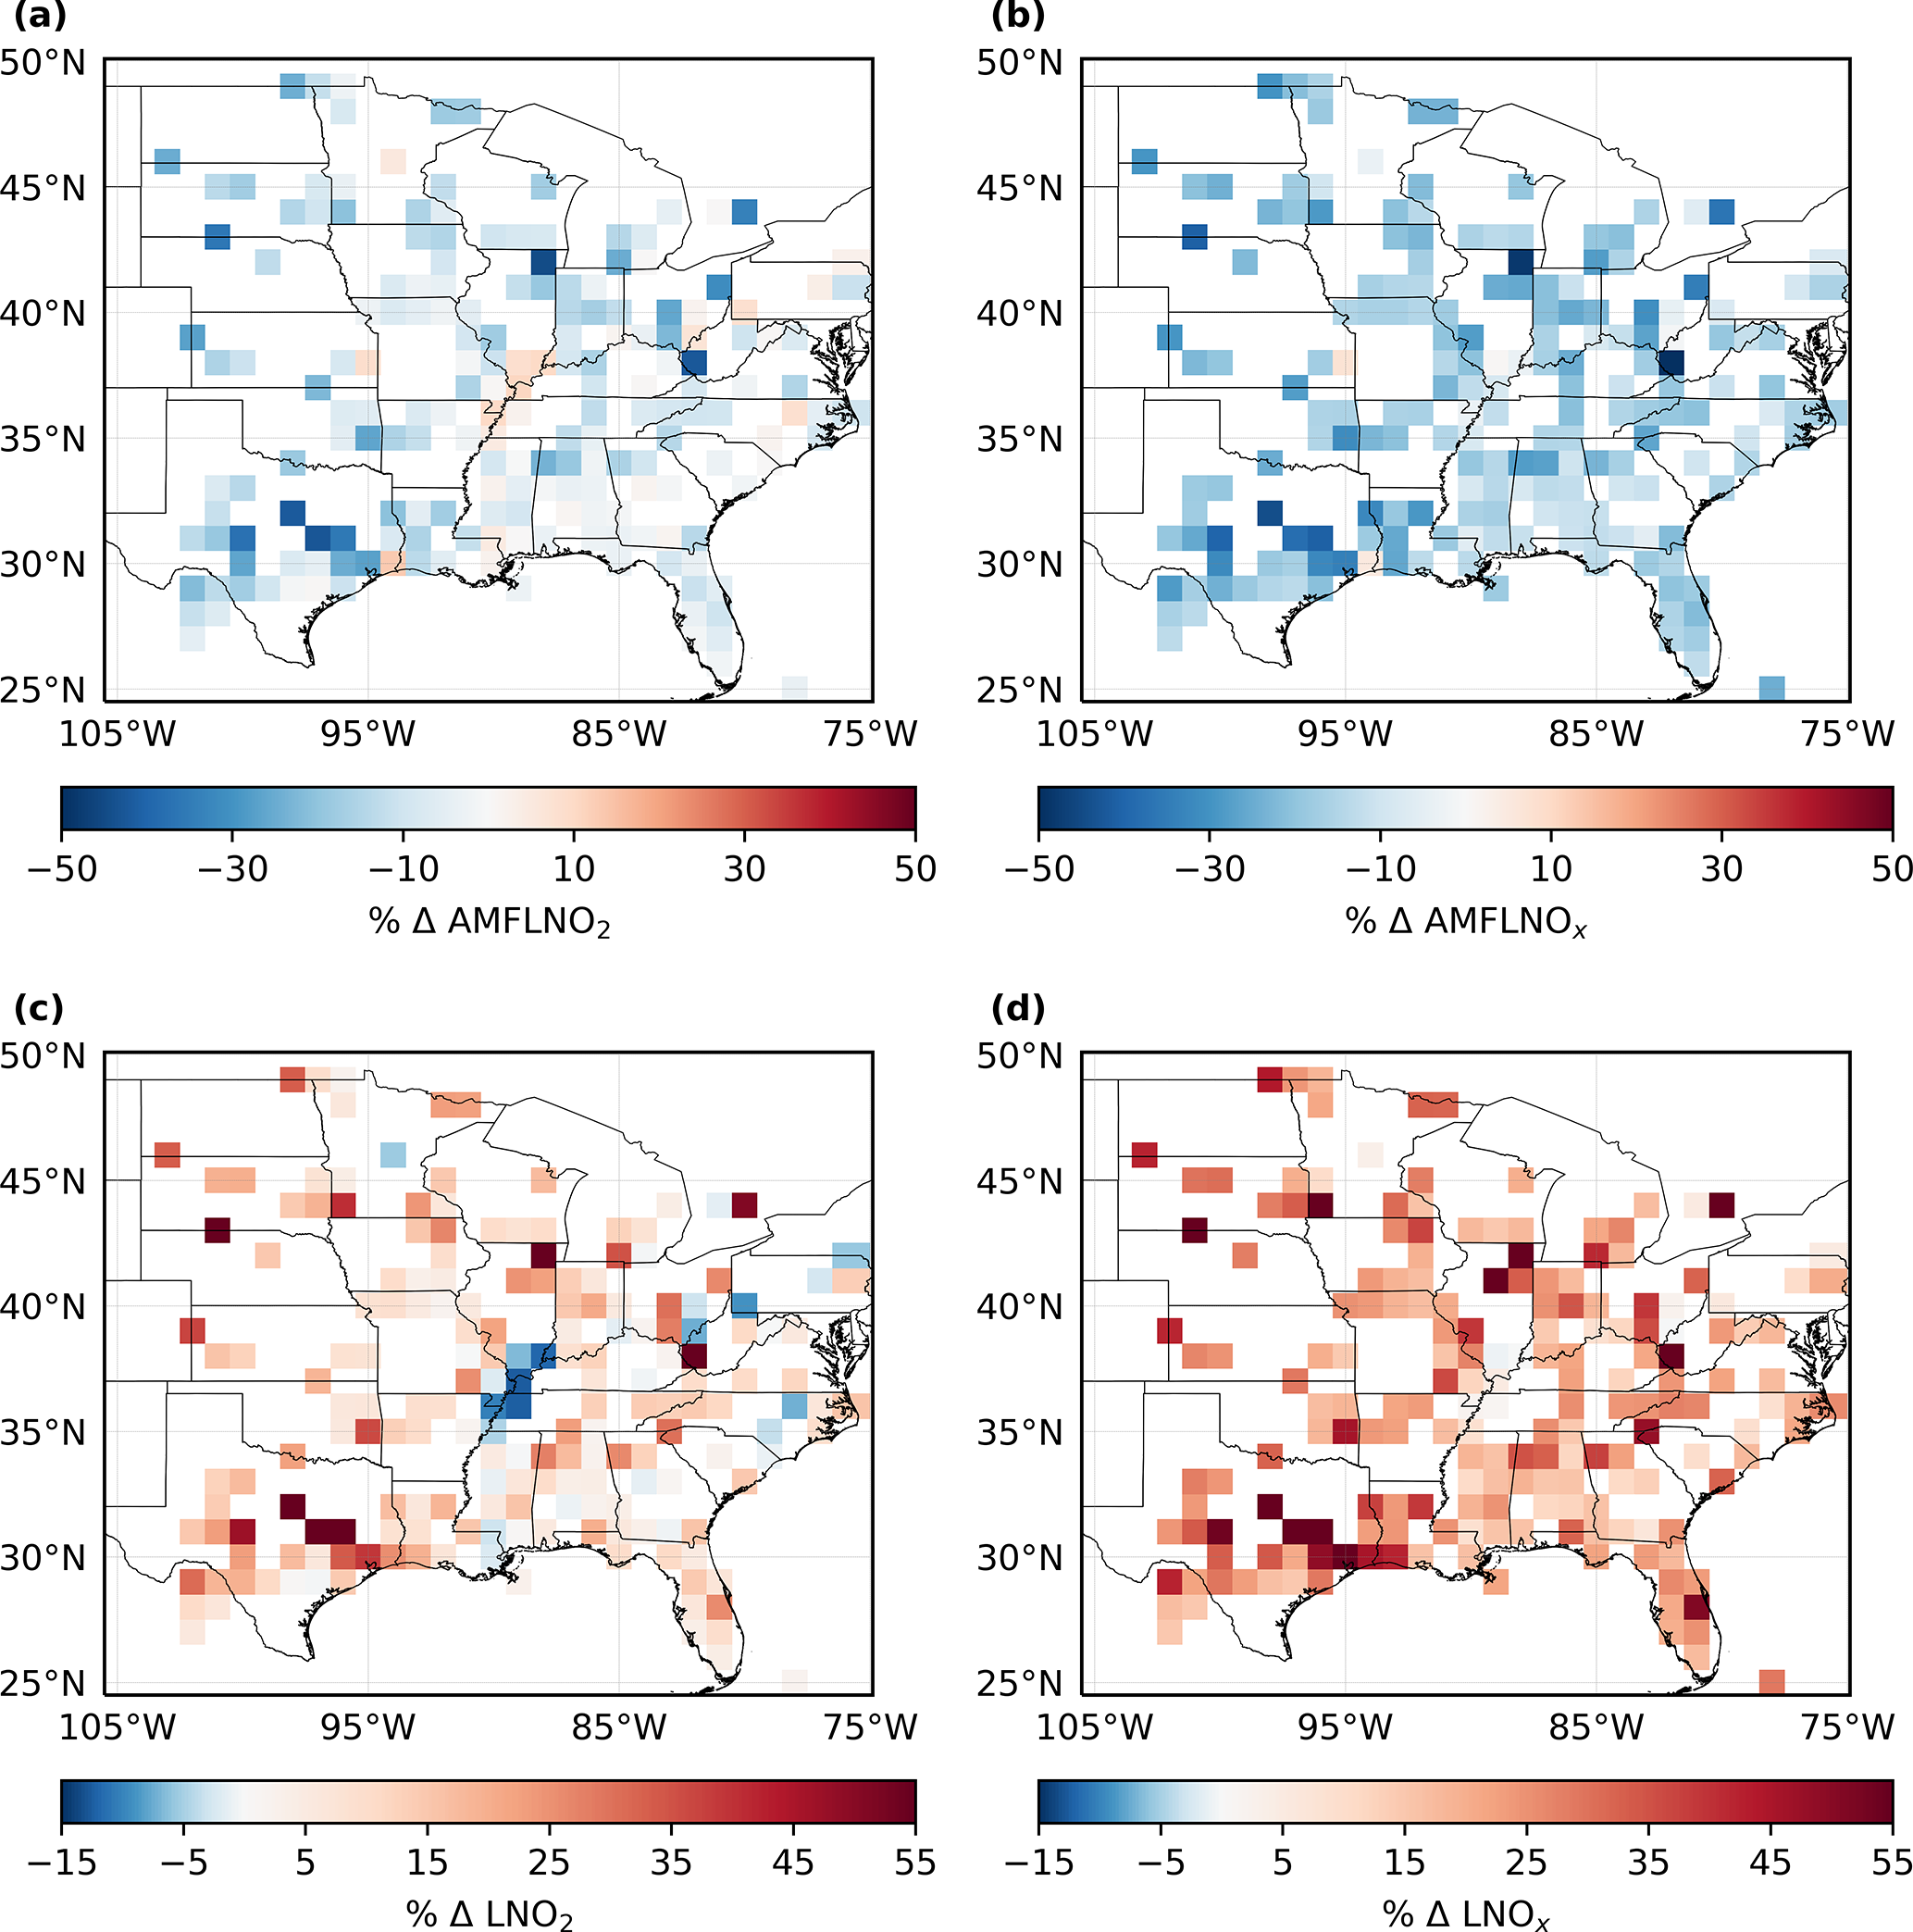
\includegraphics[width=12cm]{amt-2019-372-f10.png}
    \caption{Average percent differences in \textbf{(a)}~AMF$_{\chem{LNO_2}}$, \textbf{(b)}~AMF$_{\chem{LNO_\mathit{x}}}$, \textbf{(c)}~L\chem{NO_2}, and \textbf{(d)}~L\chem{NO_\mathit{x}} with CRF~$\geq 90$\,{\%} over MJJA 2014.
    Differences between profiles are generated by $2\times500$ and $1\times200$\,mol\,NO per flash.}
    \label{fig:simulation_diff}
\end{figure*}
To clarify this, we applied the same sensitivity test of different simulating LNO amounts for all four methods mentioned in Sect.~\ref{section:AMF}: L\chem{NO_2}, L\chem{NO_2}Vis, L\chem{NO_2}Clean, and \chem{NO_2}Vis (Fig.~\ref{fig:diff_crf100}).
Note that the threshold for CRF is set to 100\,{\%} to simplify Eq.~(\ref{AMFLNOx}) to Eq.~(\ref{AMFLNO2_crf100}).
The overall differences of L\chem{NO_2}Clean and \chem{NO_2}Vis are smaller than those of L\chem{NO_2} and L\chem{NO_2}Vis.
Comparing the numerator and denominator in the equations, it is clear why the impact of different simulating LNO amounts is smaller in Fig.~\ref{fig:diff_crf100}c and~d.
For L\chem{NO_2}Clean and \chem{NO_2}Vis, both the SCD and VCD will increase (decrease) when more (less) L\chem{NO_2} or \chem{NO_2} presents.
The difference between Fig.~\ref{fig:diff_crf100}a and~b is the denominator: the total tropospheric L\chem{NO_2} vertical column and visible L\chem{NO_2} vertical column, respectively.
As a result, the negative values in Fig.~\ref{fig:diff_crf100}a are caused by the part of L\chem{NO_2} below the cloud.
The uncertainty of retrieved L\chem{NO_2} and L\chem{NO_\mathit{x}} PEs is driven by this error, and we conservatively estimate this to be $\pm 13$\,{\%} and $\pm 25$\,{\%}, respectively.



%f11
\begin{figure*}[t]
    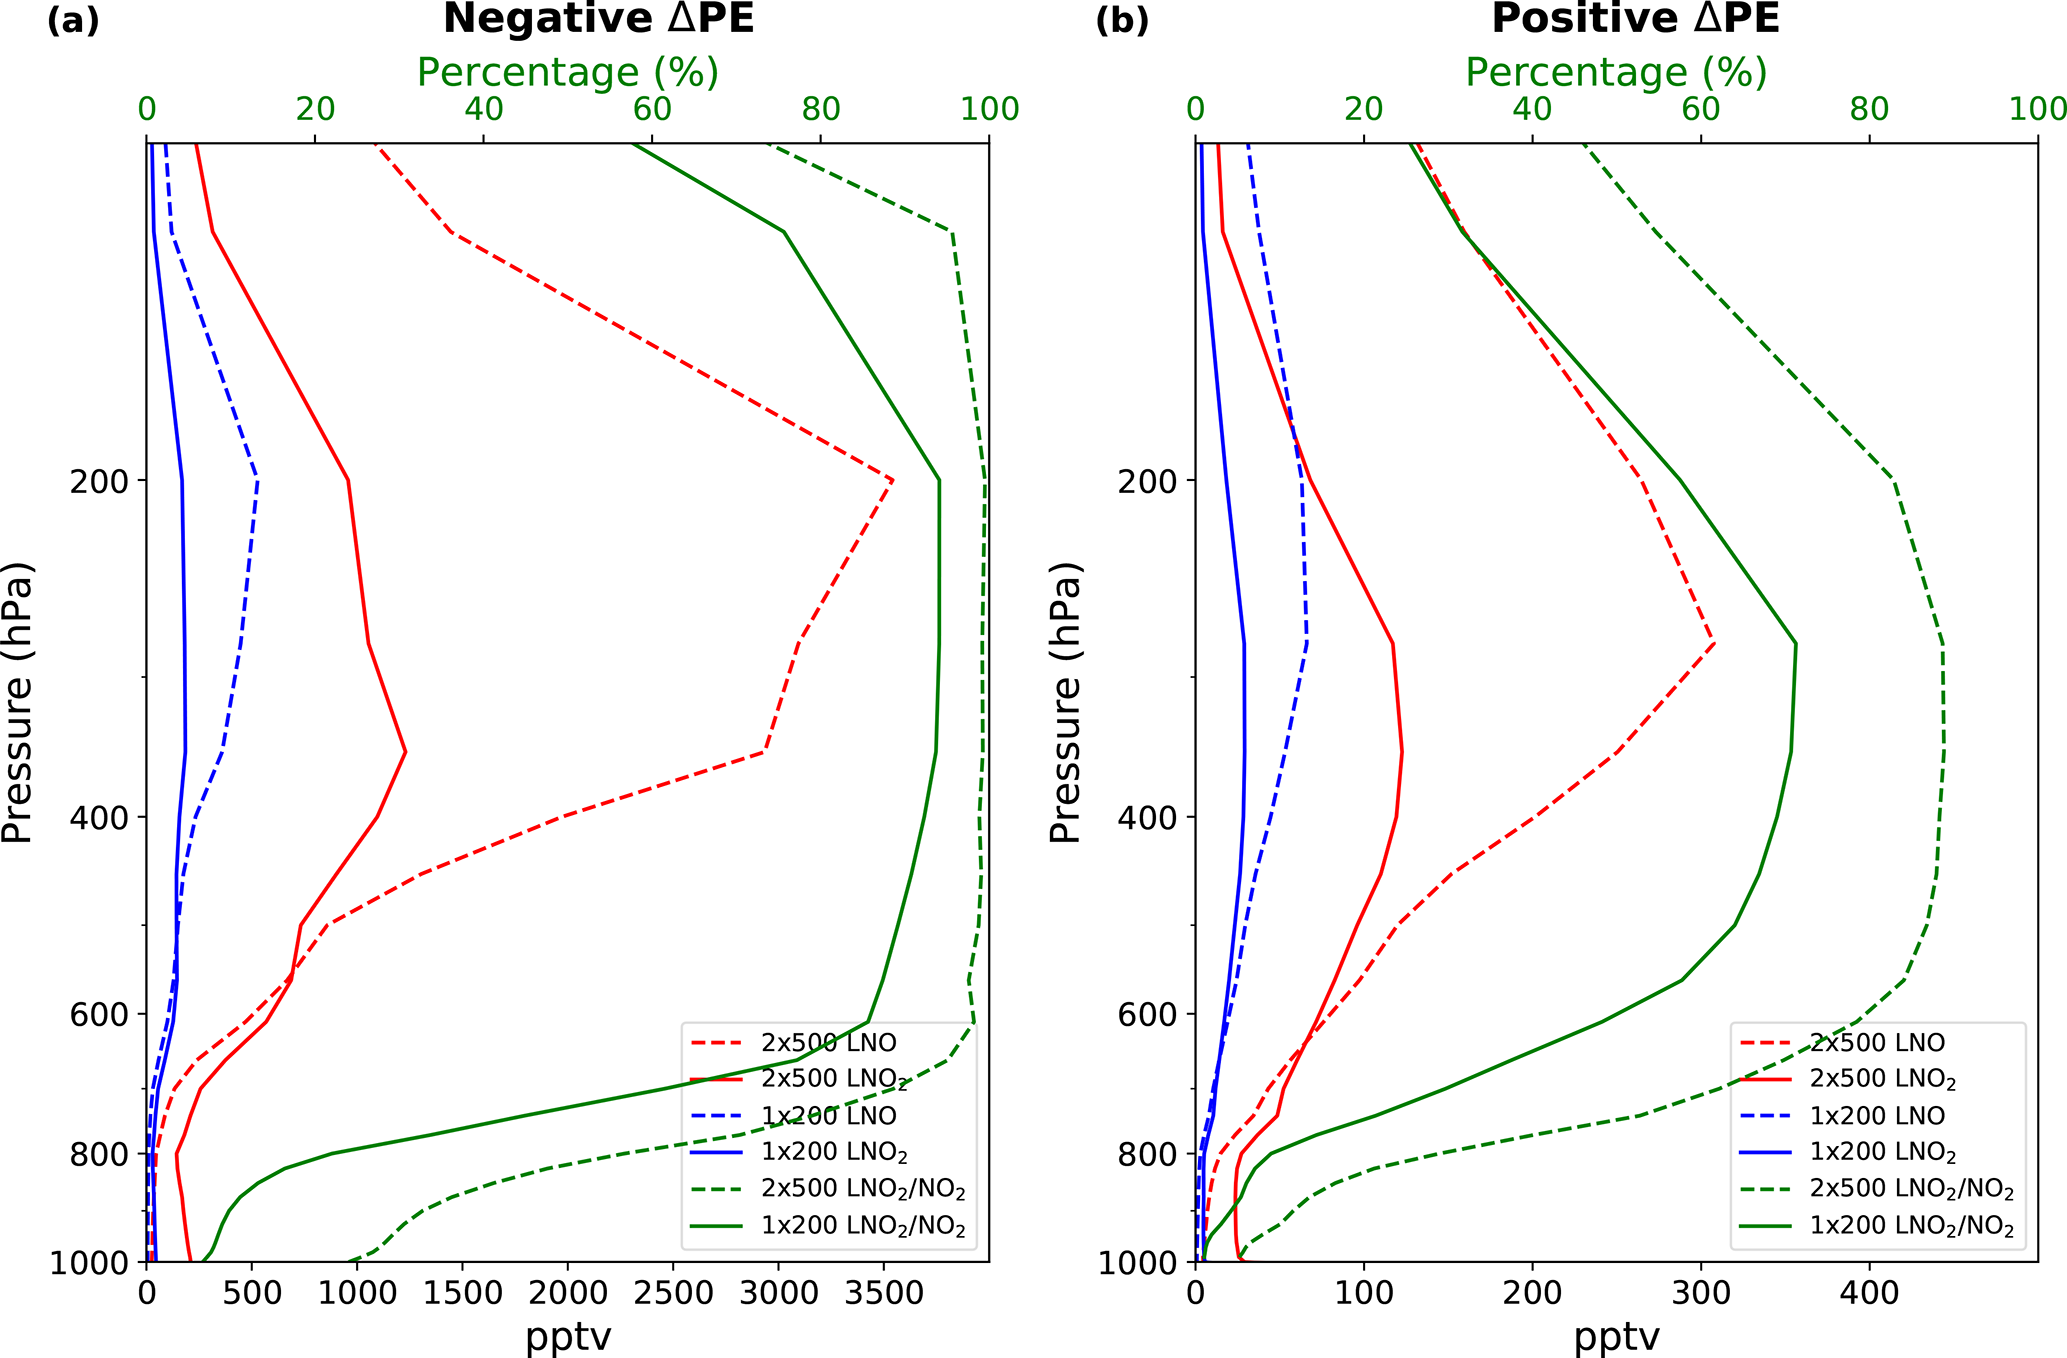
\includegraphics[width=13cm]{amt-2019-372-f11.png}
    \caption{LNO and L\chem{NO_2} profiles with different LNO settings in \textbf{(a)}~the region containing the minimal negative percent change in L\chem{NO_2} and \textbf{(b)}~the region containing the largest positive percent change in L\chem{NO_2} when the LNO setting is changed from $1\times200$ to $2\times500$\,mol\,NO per flash, averaged over MJJA 2014.
    The profiles using $1\times200$ ($2\times500$)\,mol\,NO per flash are shown in blue (red) lines.
    Solid (dashed) green lines are the mean ratio of L\chem{NO_2} to \chem{NO_2} with $1\times200$ ($2\times500$)\,mol\,NO per flash.}
    \label{fig:distribution}
\end{figure*}

%f12
\begin{figure*}[t]
    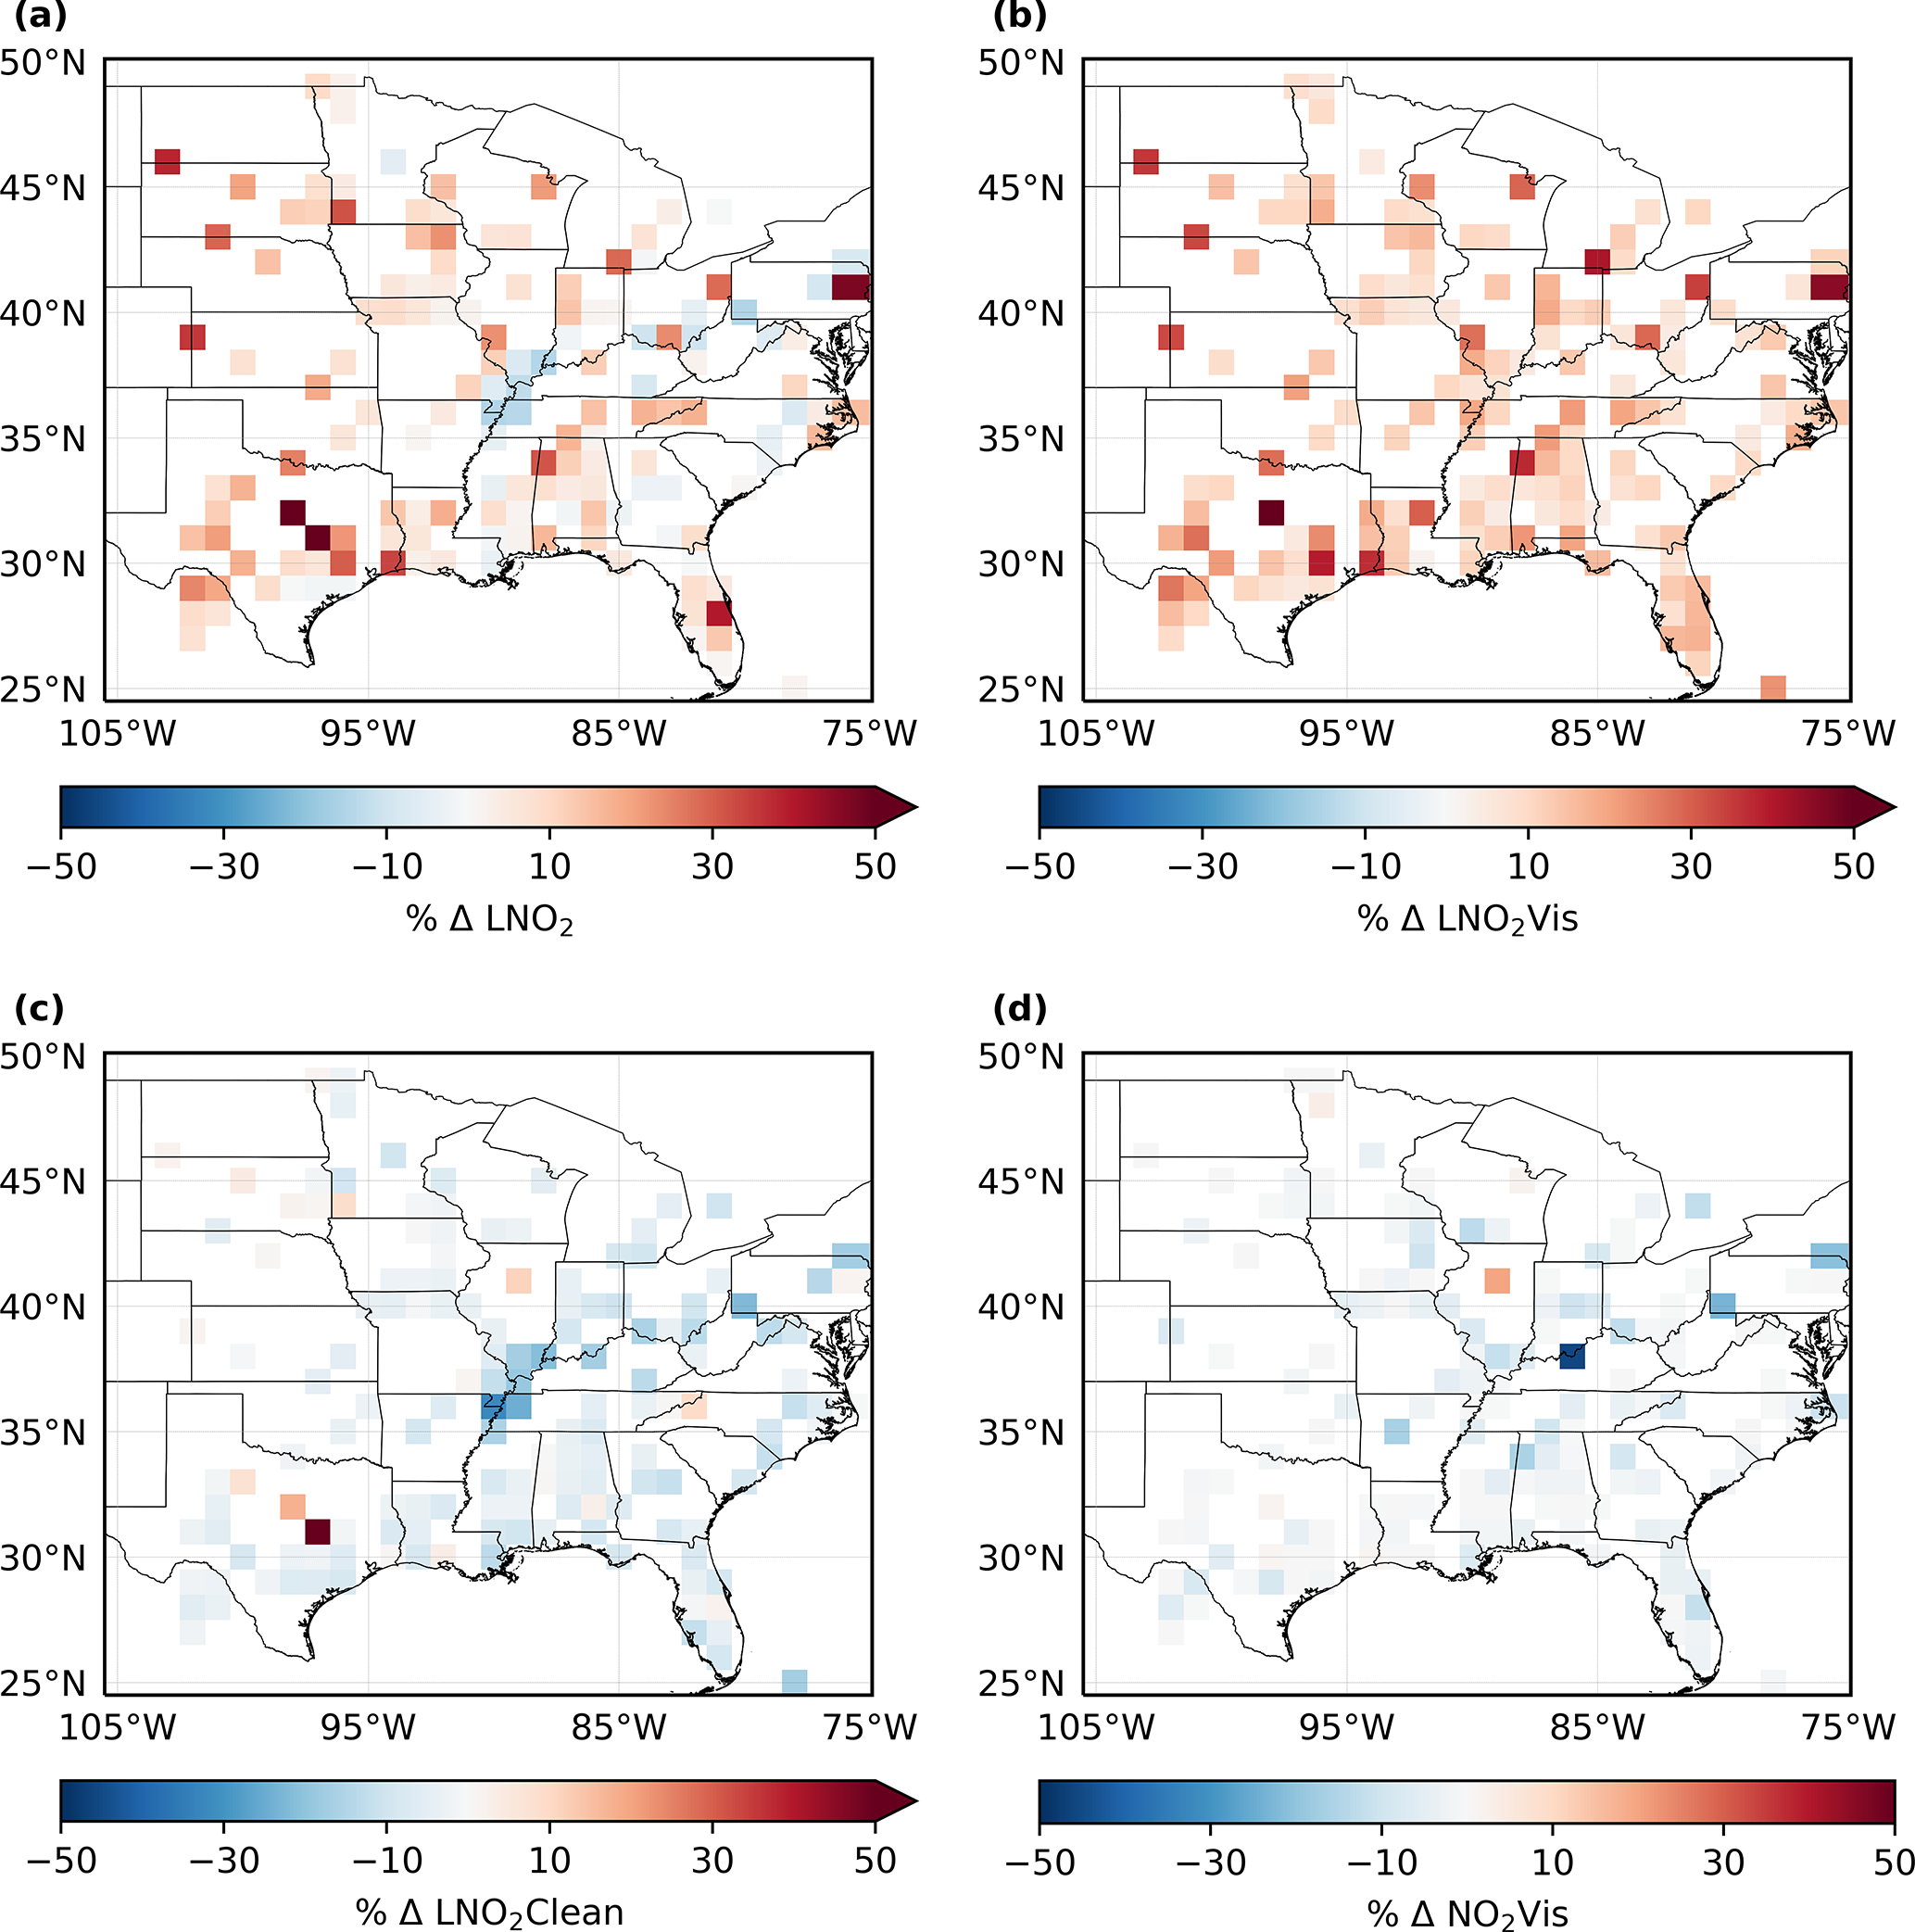
\includegraphics[width=12cm]{amt-2019-372-f12.png}
    \caption{Average percent differences in \textbf{(a)}~L\chem{NO_2}, \textbf{(b)}~L\chem{NO_2}Vis, \textbf{(c)}~L\chem{NO_2}Clean, and \textbf{(d)}~\chem{NO_2}Vis with CRF~$= 100$\,{\%} over MJJA 2014.}
    \label{fig:diff_crf100}
\end{figure*}

\section{Uncertainty analysis} \label{section:Uncertainties}

The uncertainties of the L\chem{NO_2} and L\chem{NO_\mathit{x}} PEs are estimated following \citet{Pickering.2016}, \citet{Allen.2019}, \citet{Bucsela.2019}, \citet{Laughner.2019}
and \citet{Lapierre.2020}.
We determine the uncertainty due to BEHR tropopause pressure, cloud radiance fraction, cloud pressure, surface pressure, surface reflectivity, profile shape, profile location, V$_\mathrm{strat}$, the detection efficiency of lightning, $t_\mathrm{window}$, and L\chem{NO_2} lifetime numerically by perturbing each parameter in turn and re-retrieving the L\chem{NO_2} and L\chem{NO_\mathit{x}} with the perturbed values (Table~\ref{table:Uncertainties}).

%t5
\begin{table*}[t]
    \caption{Uncertainties for the estimation of L\chem{NO_2} per flash, L\chem{NO_\mathit{x}} per flash, L\chem{NO_2} per stroke, and L\chem{NO_\mathit{x}} per stroke.}
    \begin{tabular}{llrrrr}
        \tophline
        {Type} & {Perturbation} & {L\chem{NO_2}} & {L\chem{NO_\mathit{x}}} & {L\chem{NO_2}} & {L\chem{NO_\mathit{x}}} \\

        &&per flash$^5$&per flash$^5$&per stroke$^5$&per stroke$^5$\\
        \middlehline
        BEHR tropopause pressure$^1$          & NASA product tropopause              & 6   & 4   & 6   & 4 \\
        Cloud radiance fraction$^1$           & $\pm 5$\,{\%}                            & 2   & 2   & 2   & 2 \\
        Cloud pressure$^2$                    & Variable                             & 32  & 34  & 32  & 34 \\
        Surface pressure$^1$                  & $\pm 1.5$\,{\%}                          & 0   & 0   & 0   & 0 \\
        Surface reflectivity$^1$              & $\pm 17$\,{\%}                           & 0   & 0   & 0   & 0 \\
        L\chem{NO_2} profile$^1$          & $2\times500$\,mol\,NO per flash     & 13  & 25  & 13  & 25 \\
        Profile location$^1$                  & Quasi-Monte Carlo                    & 0   & 1   & 0   & 1 \\
        Lightning detection efficiency$^3$    & IC: $\pm 16$\,{\%}, CG: $\pm 5$\,{\%}        & 15  & 15  & 15  & 15 \\
        $t_\mathrm{window}$%
        $^3$                                  & 2--4\,h                         & 10  & 10  & 8   & 8 \\
        L\chem{NO_\mathit{x}} lifetime%
        $^3$                                  & 2--12\,h                        & 24  & 24  & 24  & 24 \\
        V$_\mathrm{strat}$%
        $^4$                                  & --                                    & 10  & 10  & 10  & 10 \\
        Systematic errors in slant column$^4$ & --                                    & 5   & 5   & 5   & 5 \\
        Tropospheric background$^4$           & --                                    & 10  & 10  & 10  & 10  \\
        NO/\chem{NO_2}%
        $^4$                                  & $20\,{\%}\pm 15\,{\%} $                     & 0   & 15  & 0   & 15 \\
        Net                                   & --                                    & 49  & 56  & 48  & 56 \\
        \bottomhline
    \end{tabular}
    \belowtable{PE$_\mathrm{uncertainty} =$ (Error$_\text{rising\,perturbed\,value}$ - Error$_\text{lowering\,perturbed\,value}$)/2, where Error$_\text{\*perturbed\,value} =$ (PE$_\text{\* perturbed\,value}$ -- PE$_\text{original\,value}$)/PE$_\text{original\,value}$.
     $^1$~\citet{Laughner.2019}.
     $^2$~\citet{Acarreta.2004}. $^3$~\citet{Lapierre.2020}. $^4$~\citet{Allen.2019} and \citet{Bucsela.2019}. $^5$~Uncertainty ({\%}).}
    \label{table:Uncertainties}
\end{table*}

The GEOS-5 monthly tropopause pressure, which is consistent with the NASA standard product, is applied instead of the variable WRF tropopause height to evaluate the uncertainty (6\,{\%} for L\chem{NO_2} PE and 4\,{\%} for L\chem{NO_\mathit{x}} PE) caused by the BEHR tropopause pressure.
The cloud pressure bias is given as a function of cloud pressure and fraction by \citet{Acarreta.2004}, implying an uncertainty of 32\,{\%}, the most likely uncertainty in the production analysis, for L\chem{NO_2} PE and 34\,{\%} for L\chem{NO_\mathit{x}} PE.
The resolution of GLOBE terrain height data is much higher than the OMI pixel, and a fixed scale height is assumed in the BEHR algorithm.
As a result, \citet{Laughner.2019}
compared the average WRF surface pressures to the GLOBE surface pressures and arrived at the largest bias of 1.5\,{\%}.
Based on the largest bias, we vary the surface pressure (limited to less than 1020\,hPa), and the uncertainty can be neglected.

The error in cloud radiance fraction is transformed from cloud fraction using
\begin{equation}
\sigma = 0.05 \cdot \left.\frac{\partial{f_\mathrm{r}}}{\partial{f_\mathrm{g}}}\right|_{f_\mathrm{g,pix}},
\end{equation}
where $f_\mathrm{r}$ is the cloud radiance fraction, $f_\mathrm{g}$ is the cloud fraction, and $f_\mathrm{g,pix}$ is the cloud fraction of a specific pixel.
We calculate $\partial{f_\mathrm{r}}/\partial{f_\mathrm{g}}$ under $f_\mathrm{g,pix}$ by the relationship between all binned $f_\mathrm{r}$ and $f_\mathrm{g}$ with the increment of 0.05 for the each specific OMI orbit.
Considering the relationship, the error in cloud fraction is converted to an error in cloud radiance fraction of 2\,{\%} for the L\chem{NO_2} and L\chem{NO_\mathit{x}} PEs.

The accuracy of the 500\,m MODIS albedo product is usually within 5\,{\%} of albedo observations at the validation sites, and those exceptions with low-quality flags have been found to be primarily within 10\,{\%} of the field data \citep{Schaaf.2011}.
Since we use the bidirectional reflectance distribution function (BRDF) data directly, rather than including a radiative transfer model, 14\,{\%} Lambertian equivalent reflectivity (LER) error and 10\,{\%} uncertainty are combined to get a perturbation of 17\,{\%} \citep{Laughner.2019}.
The uncertainty due to surface reflectivity can be neglected with the 17\,{\%} perturbation.

As discussed at the end of Sect.~\ref{section:Effectsofcloud}, another setting of L\chem{NO_2} ($2\times500$\,mol\,NO per flash) is applied to determine the uncertainty of the lightning parameterization and the vertical distribution of LNO in WRF-Chem.
Differences between the two profiles lead to an uncertainty of 13\,{\%} and 25\,{\%} in the resulting PEs of L\chem{NO_2} and L\chem{NO_\mathit{x}}.
Another sensitivity test allows each pixel to shift by $-0.2$, 0, or $+0.2$\,{\degree} in the directions of longitude and latitude, taking advantage of the high-resolution profile location in WRF-Chem.
The resulting uncertainty of L\chem{NO_\mathit{x}} PE is 1\,{\%}, including the error of transport and chemistry by shifting pixels.

Compared to the NASA standard product v2, \citet{Krotkov.2017} demonstrated that the noise in V$_\mathrm{strat}$ is $1 \times 10^{14}$\,cm$^{-2}$.
Errors in polluted regions can be slightly larger than this value, while errors in the cleanest areas are typically significantly smaller \citep{Bucsela.2013}.
We estimated the uncertainty of the V$_\mathrm{strat}$ component and the slant column errors to be 10\,{\%} and 5\,{\%}, respectively, following \citet{Allen.2019}.

Based on the standard deviation of the detection efficiency estimation over the CONUS relative to LIS, ENTLN detection efficiency uncertainties are $\pm$ 16\,{\%} for total and IC flashes and strokes.
Due to the high detection efficiency of CG over the CONUS, the uncertainty is estimated to be $\pm 5$\,{\%} \citep{Lapierre.2020}.
It is found that the resulting uncertainty of detection efficiency is 15\,{\%} in the production analysis.
We have used the $t_\mathrm{window}$ of 2.4\,h for counting ENTLN flashes and strokes to analyze L\chem{NO_2} and L\chem{NO_\mathit{x}} production.
Because $t_\mathrm{window}$ derived from the ERA5 reanalysis can not represent the variable wind speeds, a sensitivity test is performed which yields an uncertainty of 10\,{\%} for production per flash and 8\,{\%} for production per stroke using $t_\mathrm{window}$ of 2 and 4\,h.
Meanwhile, the lifetime of UT \chem{NO_\mathit{x}} ranges from 2 to 12\,h depending on the convective location, the methyl peroxy nitrate and alkyl, and multifunctional nitrates \citep{Nault.2017}.
The lifetime ($\tau$) of \chem{NO_2} in Eq.~(\ref{inition}) is replaced by 2 and 12\,h to determine the uncertainty as 24\,{\%} due to lifetime.
This is comparable with the uncertainty (25\,{\%}) caused by lightning parameterization for the L\chem{NO_\mathit{x}} type.

Recent studies revealed that the modeled \chem{NO/NO_2} ratio departs from the data in the SEAC$^{4}$RS aircraft campaign \citep{Travis.2016,Silvern.2018}.
\citet{Silvern.2018} attributed this to the positive interference on the \chem{NO_2} measurements or errors in the cold-temperature \chem{NO-NO_2-O_3} photochemical reaction rate.
We assign a 20\,{\%} bias with $\pm 15$\,{\%} uncertainty to this error considering the possible positive \chem{NO_2} measurement interferences \citep{Allen.2019,Bucsela.2019} and estimate the uncertainty to be 15\,{\%} for L\chem{NO_\mathit{x}} PE.

In addition, the estimation of L\chem{NO_\mathit{x}} PE also depends on the tropospheric background \chem{NO_2}.
In our method, the main factors affecting this factor are the emissions inventory and the amount of transported \chem{NO_2}.
For the emissions inventory, the sources of uncertainty are assumptions, methods, input data, and calculation errors.
As a result, the uncertainties for different species or pollutants related to \chem{NO_2} are different and the U.S. EPA also does not publish the quantified uncertainty measures because the parties that submit emissions estimates to the U.S. EPA are not asked to include quantitative uncertainty measurements or estimates \citep{us20152011}.
For the simulated convective transport, \citet{Li.2018} compared the cloud-resolving simulations with these based on convective parameterization and pointed out that the convective transport was weaker in the parameterization.
But, we believe that the ratio condition (L\chem{NO_2}Vis/\chem{NO_2}Vis $\geq 50$\,{\%}) should reduce these two kinds of uncertainty, and we assume an uncertainty of 10\,{\%}, which is less than the 20\,{\%} assigned in \citet{Allen.2019} and \citet{Bucsela.2019}.

The overall uncertainty is estimated as the square root of the sum of the squares of all individual uncertainties in Table~\ref{table:Uncertainties}.
The net uncertainty is 48\,{\%} and 56\,{\%} for the L\chem{NO_2} type and L\chem{NO_\mathit{x}} type, respectively.
The mean L\chem{NO_2} per flash, L\chem{NO_\mathit{x}} per flash, L\chem{NO_2} per stroke, and L\chem{NO_\mathit{x}} per stroke based on the linear regression and summation method are 32\,mol per flash, 90\,mol per flash, 6\,mol per stroke, and 17\,mol per stroke.
Applying the corresponding uncertainty to these mean values, we arrive at $32 \pm 15$\,mol L\chem{NO_2} per flash, $90 \pm 50$\,mol L\chem{NO_\mathit{x}} per flash, $6 \pm 3$\,mol L\chem{NO_2} per stroke, and $17 \pm 10$\,mol L\chem{NO_\mathit{x}} per stroke.
This is in the range of current literature estimates ranging from 33 to 500\,mol L\chem{NO_\mathit{x}} per flash \citep{Schumann.2007,Beirle.2010,Bucsela.2010}.
\citet{Bucsela.2010} estimated L\chem{NO_\mathit{x}} PE of 100--250\,mol per flash, which is higher than but overlaps with our estimate.
\citet{Pickering.2016} estimated L\chem{NO_\mathit{x}} PE to be $80 \pm 45$\,mol per flash for the Gulf of Mexico.
This is 50\,{\%} smaller than our flash-based results over the CONUS, if we use the same linear regression method which is based on the daily summed values instead of daily mean values.
Note that the criteria defined in Sect.~\ref{section:Criteria} lead to many missing data over the Gulf of Mexico; thus it is actually a comparison between different regions.
For the stroke-based results, \citet{Lapierre.2020} found lower L\chem{NO_2} PE of $1.6 \pm 0.1$\,mol per stroke, and the difference is caused by the different version of BEHR algorithm and several settings as mentioned in Sect.~\ref{section:Comparison}.
\citet{Bucsela.2019} inferred an average value of $200 \pm 110$\,mol (122\,{\%} larger than our results) of L\chem{NO_\mathit{x}} produced per flash over the North America, this is related to the different algorithm, lightning data, and lightning thresholds.

\conclusions \label{section:conclusions}

In this study, a new algorithm for retrieving L\chem{NO_2} (L\chem{NO_\mathit{x}}) from OMI, including L\chem{NO_2} (L\chem{NO_\mathit{x}}) below cloud, has been developed for application over active convection.
It works in both clean and polluted regions because of the consideration of tropospheric background pollution in the definition of AMFs.
It uses specific criteria combined with several other conditions (sufficient CRF, coincident ENTLN data, TL~$\geq 1000$, and ratio $\geq 50$\,{\%}) to ensure that the electrically active regions are detected by OMI and simulated by WRF-Chem successfully.
We conducted an analysis on $1{\degree} \times 1{\degree}$ daily boxes in MJJA 2014 and obtained the seasonal mean L\chem{NO_2} and L\chem{NO_\mathit{x}} production efficiencies over the CONUS.
Considering all the uncertainties (Table~\ref{table:Uncertainties}) and applying the summation and regression methods, the final mean production efficiencies are estimated to be $32 \pm 15$\,mol L\chem{NO_2} per flash, $90 \pm 50$\,mol L\chem{NO_\mathit{x}} per flash, $6 \pm 3$\,mol L\chem{NO_2} per stroke, and $17 \pm 10$\,mol L\chem{NO_\mathit{x}} per stroke.

Compared with \citet{Lapierre.2020}, we find that the L\chem{NO_2} production could be larger when the below-cloud L\chem{NO_2} is taken into account, especially for the high clouds.
Meanwhile, if the method of \citet{Pickering.2016} is applied without the background \chem{NO_2} correction, the derived L\chem{NO_\mathit{x}} production efficiency is similar to ours in clean regions or regions with a high L\chem{NO_2} concentration above the cloud, but it could be overestimated by more than 18\,{\%} in polluted regions.
Finally, implementing profiles generated with different model settings of lightning ($1\times200$ and $2\times500$\,mol\,NO per flash), we find that the larger LNO production setting leads to 62\,{\%} larger retrieval of L\chem{NO_\mathit{x}} on average despite some regionally dependent effects caused by the nonlinear calculation of AMF.
Both the ratio of the tropospheric L\chem{NO_2} above the cloud to the total tropospheric L\chem{NO_2} and the ratio of L\chem{NO_2} to \chem{NO_2} cause different comprehensive effects due to the nonlinear calculation of AMF$_{\chem{LNO_2}}$ and AMF$_{\chem{LNO_\mathit{x}}}$.


\hack{\newpage}
Since other regions, like China and India, have much more \chem{NO_2} pollution than the CONUS, it is necessary to consider the background \chem{NO_2} in detail.
These analyses will be complemented by the recently launched satellite instrument (TROPOspheric Monitoring Instrument, TROPOMI) \citep{Veefkind.2012,Boersma.2018,Griffin.2019} and Lightning Mapping Imager (LMI) on the new-generation Chinese geostationary meteorological satellite Fengyun-4 \citep{Min.2017,Yang.2017,Zhang.2019}.
Future work investigating the flash channel length and more detailed lightning parameterization in WRF-Chem would greatly benefit L\chem{NO_\mathit{x}} estimation.
Applying current methods in future studies may enhance the accuracy of L\chem{NO_\mathit{x}} production at both local and global scales.

\hack{\clearpage}

\appendix
\section{AMF definitions used in this study} \label{AppendixA}

\begin{gather}
\mathrm{AMF}_{\chem{LNO_2}} = \displaystyle{{(1-f_\mathrm{r}) \int_{p_\mathrm{surf}}^{p_\mathrm{ tp}} w_\mathrm{clear}(p) \chem{NO_2}(p) \: \mathrm{d}p \atop+ f_\mathrm{r} \int_{p_\mathrm{cloud}}^{p_\mathrm{tp}} w_\mathrm{cloudy}(p) \chem{NO_2}(p) \: \mathrm{d}p}\over{\int_{p_\mathrm{surf}}^{p_\mathrm{tp}} \chem{LNO_2}(p) \: \mathrm{d}p}}\\
\mathrm{AMF}_{\chem{LNO_\mathit{x}}} = \displaystyle{{(1-f_\mathrm{r}) \int_{p_\mathrm{surf}}^{p_\mathrm{tp}} w_\mathrm{clear}(p) \chem{NO_2}(p) \: \mathrm{d}p \atop+ f_\mathrm{r} \int_{p_\mathrm{cloud}}^{p_\mathrm{tp}} w_\mathrm{cloudy}(p) \chem{NO_2}(p) \: \mathrm{d}p}\over{\int_{p_\mathrm{surf}}^{p_\mathrm{tp}} \chem{LNO_\mathit{x}}(p) \: \mathrm{d}p}}
\end{gather}
Here $f_\mathrm{r}$ is the cloud radiance fraction, $p_\mathrm{surf}$ is the surface pressure, $p_\mathrm{tp}$ is the tropopause pressure, $p_\mathrm{cloud}$ is the cloud optical pressure (CP), $w_\mathrm{clear}$ and $w_\mathrm{cloudy}$ are respectively the pressure-dependent scattering weights from the TOMRAD lookup table \citep{Bucsela.2013}  for clear and cloudy parts, and \chem{NO_2}$(p)$ is the modeled \chem{NO_2} vertical profile.
\chem{LNO_{2}}$(p)$ and L\chem{NO_\mathit{x}}$(p)$ are respectively the L\chem{NO_2} and L\chem{NO_\mathit{x}} vertical profiles calculated by the difference of vertical profiles between WRF-Chem simulations with and without lightning.

\begin{gather}
\mathrm{AMF}_{\chem{LNO_2}\mathrm{Clean}} = \displaystyle{{(1-f_\mathrm{r}) \int_{p_{\mathrm{surf}}}^{p_{\mathrm{tp}}} w_\mathrm{{clear}}(p) \chem{LNO_2}(p) \: \mathrm{d}p \atop+ f_\mathrm{r} \int_{p_\mathrm{{cloud}}}^{p_{\mathrm{tp}}} w_{\mathrm{cloudy}}(p) \chem{LNO_2}(p) \: \mathrm{d}p}\over{\int_{p_{\mathrm{surf}}}^{p_{\mathrm{tp}}} \chem{LNO_2}(p) \: \mathrm{d}p}}\\
\mathrm{AMF}_{\chem{NO_2}\mathrm{Vis}} = \displaystyle{{(1-f_\mathrm{r}) \int_{p_{\mathrm{surf}}}^{p_{\mathrm{tp}}} w_\mathrm{{clear}}(p) \chem{NO_2}(p) \: \mathrm{d}p \atop+ f_\mathrm{r} \int_{p_\mathrm{{cloud}}}^{p_{\mathrm{tp}}} w_{\mathrm{cloudy}}(p) \chem{NO_2}(p) \: \mathrm{d}p}\over{(1-f_\mathrm{g}) \int_{p_{\mathrm{surf}}}^{p_{\mathrm{tp}}} \chem{NO_2}(p) \: \mathrm{d}p + f_\mathrm{g} \int_{p_\mathrm{{cloud}}}^{p_{\mathrm{tp}}}\atop \chem{NO_2}(p) \: \mathrm{d}p}}\\
\mathrm{AMF}_{\chem{NO_\mathit{x}}\mathrm{Vis}} = \displaystyle{{(1-f_\mathrm{r}) \int_{p_{\mathrm{surf}}}^{p_{\mathrm{tp}}} w_\mathrm{{clear}}(p) \chem{NO_2}(p) \: \mathrm{d}p \atop+ f_\mathrm{r} \int_{p_\mathrm{{cloud}}}^{p_{\mathrm{tp}}} w_{\mathrm{cloudy}}(p) \chem{NO_2}(p) \: \mathrm{d}p}\over{(1-f_\mathrm{g}) \int_{p_{\mathrm{surf}}}^{p_{\mathrm{tp}}} \chem{NO_\mathit{x}}(p) \: \mathrm{d}p + f_\mathrm{g} \int_{p_\mathrm{{cloud}}}^{p_{\mathrm{tp}}} \atop\chem{NO_\mathit{x}}(p) \: \mathrm{d}p}}\\
\mathrm{AMF}_{\chem{LNO_2}\mathrm{Vis}} = \displaystyle{{(1-f_\mathrm{r}) \int_{p_{\mathrm{surf}}}^{p_{\mathrm{tp}}} w_\mathrm{{clear}}(p) \chem{NO_2}(p) \: \mathrm{d}p\atop + f_\mathrm{r} \int_{p_\mathrm{{cloud}}}^{p_{\mathrm{tp}}} w_{\mathrm{cloudy}}(p) \chem{NO_2}(p) \: \mathrm{d}p}\over{(1-f_\mathrm{g}) \int_{p_{\mathrm{surf}}}^{p_{\mathrm{tp}}} \chem{LNO_2}(p) \: \mathrm{d}p \atop+ f_\mathrm{g} \int_{p_\mathrm{{cloud}}}^{p_{\mathrm{tp}}} \chem{LNO_2}(p) \: \mathrm{d}p}}
\end{gather}
Here $f_\mathrm{g}$ is the geometric cloud fraction and \chem{NO_\mathit{x}}$(p)$ is the modeled \chem{NO_\mathit{x}} vertical profile.

%ta1
\begin{table}[h!]
    \caption{Simple forms of abbreviations for AMFs.}
    \begin{tabular}{lll}
        \tophline
        {Abbreviations} & {Numerator$^1$} & {Denominator$^2$} \\
        \middlehline
        AMF$_\chem{LNO_2}$          & S$_\chem{NO_2}$     & V$_\chem{LNO_2}$ \\
        AMF$_{\chem{LNO_2}\mathrm{Vis}}$       & S$_\chem{NO_2}$     & V$_{\chem{LNO_2}\mathrm{Vis}}$ \\
        AMF$_{\chem{LNO_2}\mathrm{Clean}}$     & S$_\chem{LNO_2}$    & V$_\chem{LNO_2}$ \\
        AMF$_{\chem{NO_2}\mathrm{Vis}}$        & S$_\chem{NO_2}$     & V$_{\chem{NO_2}\mathrm{Vis}}$ \\
        AMF$_\chem{LNO_\mathit{x}}$          & S$_\chem{NO_2}$     & V$_\chem{LNO_\mathit{x}}$ \\
        AMF$_{\chem{NO_\mathit{x}}\mathrm{Vis}}$        & S$_\chem{NO_2}$     & V$_{\chem{NO_\mathit{x}}\mathrm{Vis}}$ \\
        \bottomhline
    \end{tabular}
    \belowtable{$^1$~The part of simulated VCD seen by OMI. $^2$~The simulated VCD.}
    \label{table:AMFs}
\end{table}

\section{L\chem{NO_\mathit{x}} production based on lower lightning thresholds} \label{AppendixB}
While we used 2400 flashes per box and 8160 strokes per box per 2.4\,h time window for detecting L\chem{NO_\mathit{x}}, here we show results obtained when using one flash per box and 3.4 strokes per box in the same time window.
We note that the WRF total lightning threshold is also reduced to one flash per box, but we keep the ratio condition unchanged.
Briefly, the condition is CRF90\_ENTLN1(3.4)\_TL1\_ratio50 as shown in Table~\ref{table:Abbreviations}.

Similarly, the order of estimated daily PEs is L\chem{NO_2}Clean $>$ L\chem{NO_2} $>$ \chem{NO_2}Vis $>$ L\chem{NO_2}Vis (Fig.~\ref{fig:PE_linear_fewerflash}).
Compared with Fig.~\ref{fig:PE_linear}, the L\chem{NO_2} per flash and L\chem{NO_\mathit{x}} per flash are larger while PEs based on stroke data are smaller.
Considering the additional boxes of fewer lightning counts, differences in the daily mean flashes and \chem{NO_\mathit{x}} result in different PEs, and the relationship presents more like the power function as mentioned in \citet{Bucsela.2019}.

Instead of using the nonlinear regression of power function
  \begin{equation} \label{power_function}
    y = \alpha x^{\beta},
  \end{equation}
  where $x$ is flashes or strokes and $y$ is \chem{NO_2} or \chem{NO_\mathit{x}},
  we take the logarithm of both sides and apply the linear regression to data:
  \begin{equation} \label{logarithm}
    \log_{10}y = \log_{10}{\alpha} + \beta \log_{10}{x}.
  \end{equation}
As expected, the linear regression based on logarithmized data performs better in this situation and yields $\alpha = 38$\,kmol and $\beta = 0.3$ for L\chem{NO_\mathit{x}} per flash (Fig.~\ref{fig:PE_power_fewerflash}).
Since we use the unbinned data (flashes not divided into many groups), we compare our results with \citet{Bucsela.2019} based on the same kind of data ($\alpha = 10.3$\,kmol and $\beta = 0.42$).
The large difference of $\alpha$ is related to the method of estimating L\chem{NO_\mathit{x}}, different lightning data (WWLLN and ENTLN), and different regions (northern midlatitudes and CONUS).
Note that the resolution (13\,km\,$\times$\,24\,km) of OMI could weaken the signal of L\chem{NO_\mathit{x}}.
We believe the phenomenon of higher production efficiency as flash rate decreases (Fig.~\ref{fig:PE_fewerflash}) could be explored in much more detail with higher-resolution data like the TROPOMI data.

%fb1
\begin{figure*}[p]
    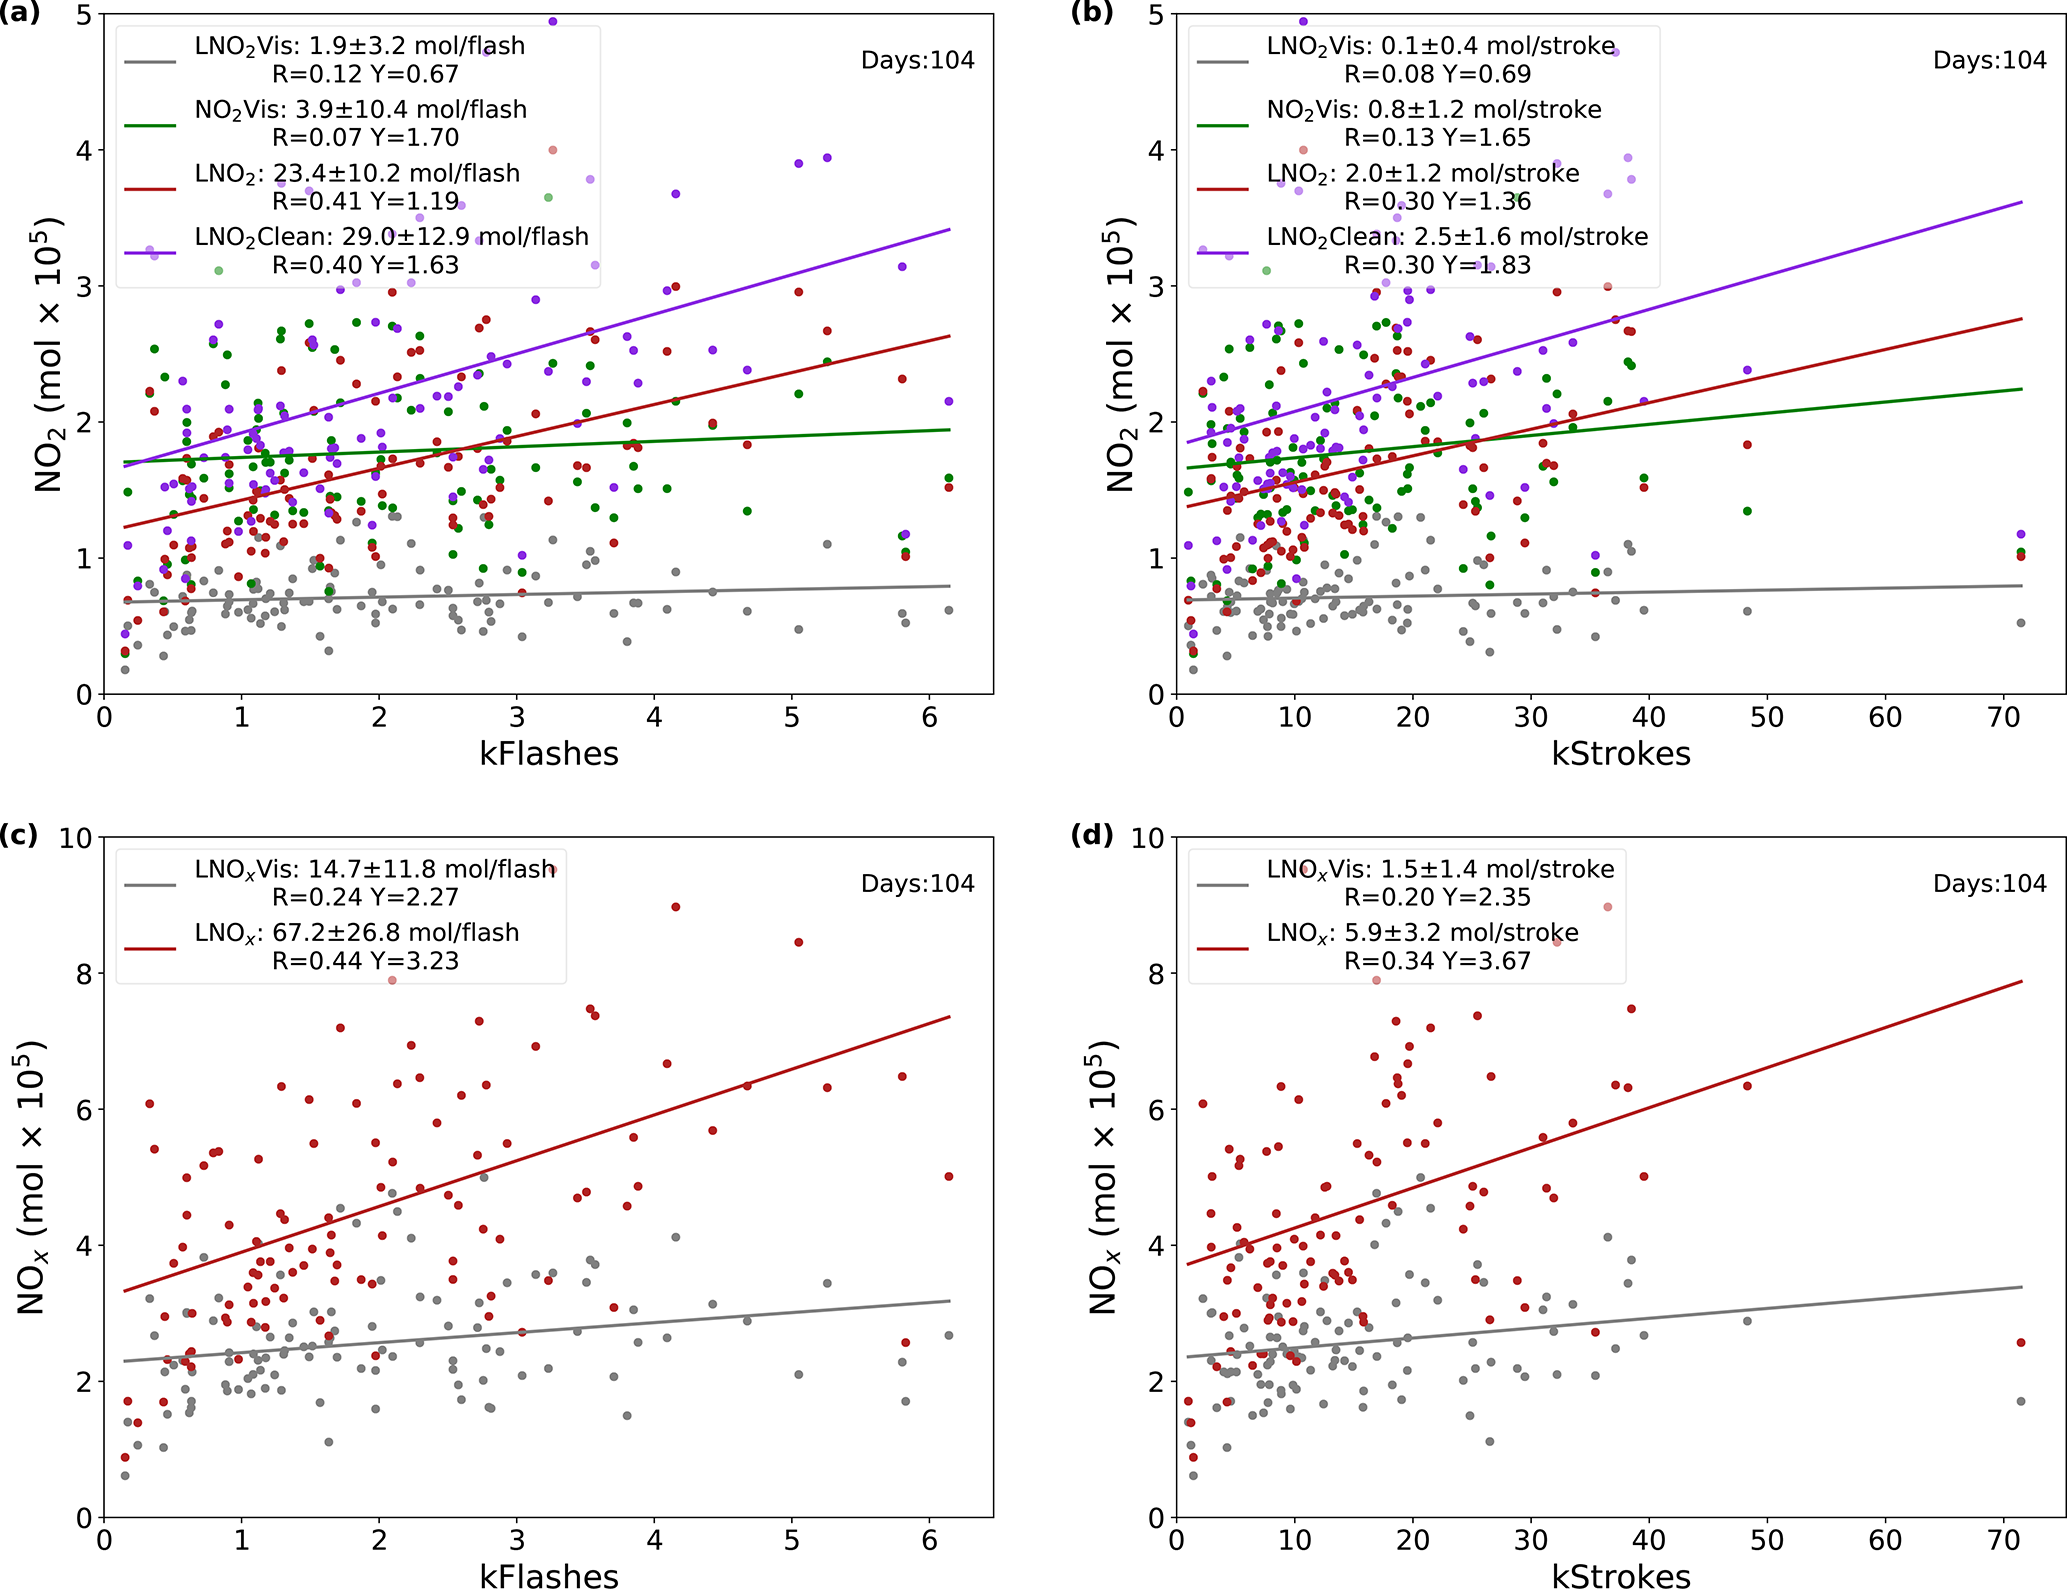
\includegraphics[width=15cm]{amt-2019-372-f13.png}
    \caption{Linear regressions with CRF~$\geq 90$\,{\%} and a flash threshold of one flash per box or 3.4 strokes per box per 2.4\,h.
  \textbf{(a)}~Daily \chem{NO_2}Vis, L\chem{NO_2}Vis, L\chem{NO_2}, and L\chem{NO_2}Clean versus ENTLN total flash data.
  \textbf{(b)}~Same as \textbf{(a)}~but for strokes.
  \textbf{(c)}~Daily L\chem{NO_\mathit{x}}Vis and L\chem{NO_\mathit{x}} versus total flashes.
  \textbf{(d)}~Same as \textbf{(c)}~but for strokes.}
    \label{fig:PE_linear_fewerflash}
\end{figure*}

%fb2
\begin{figure*}[p]
    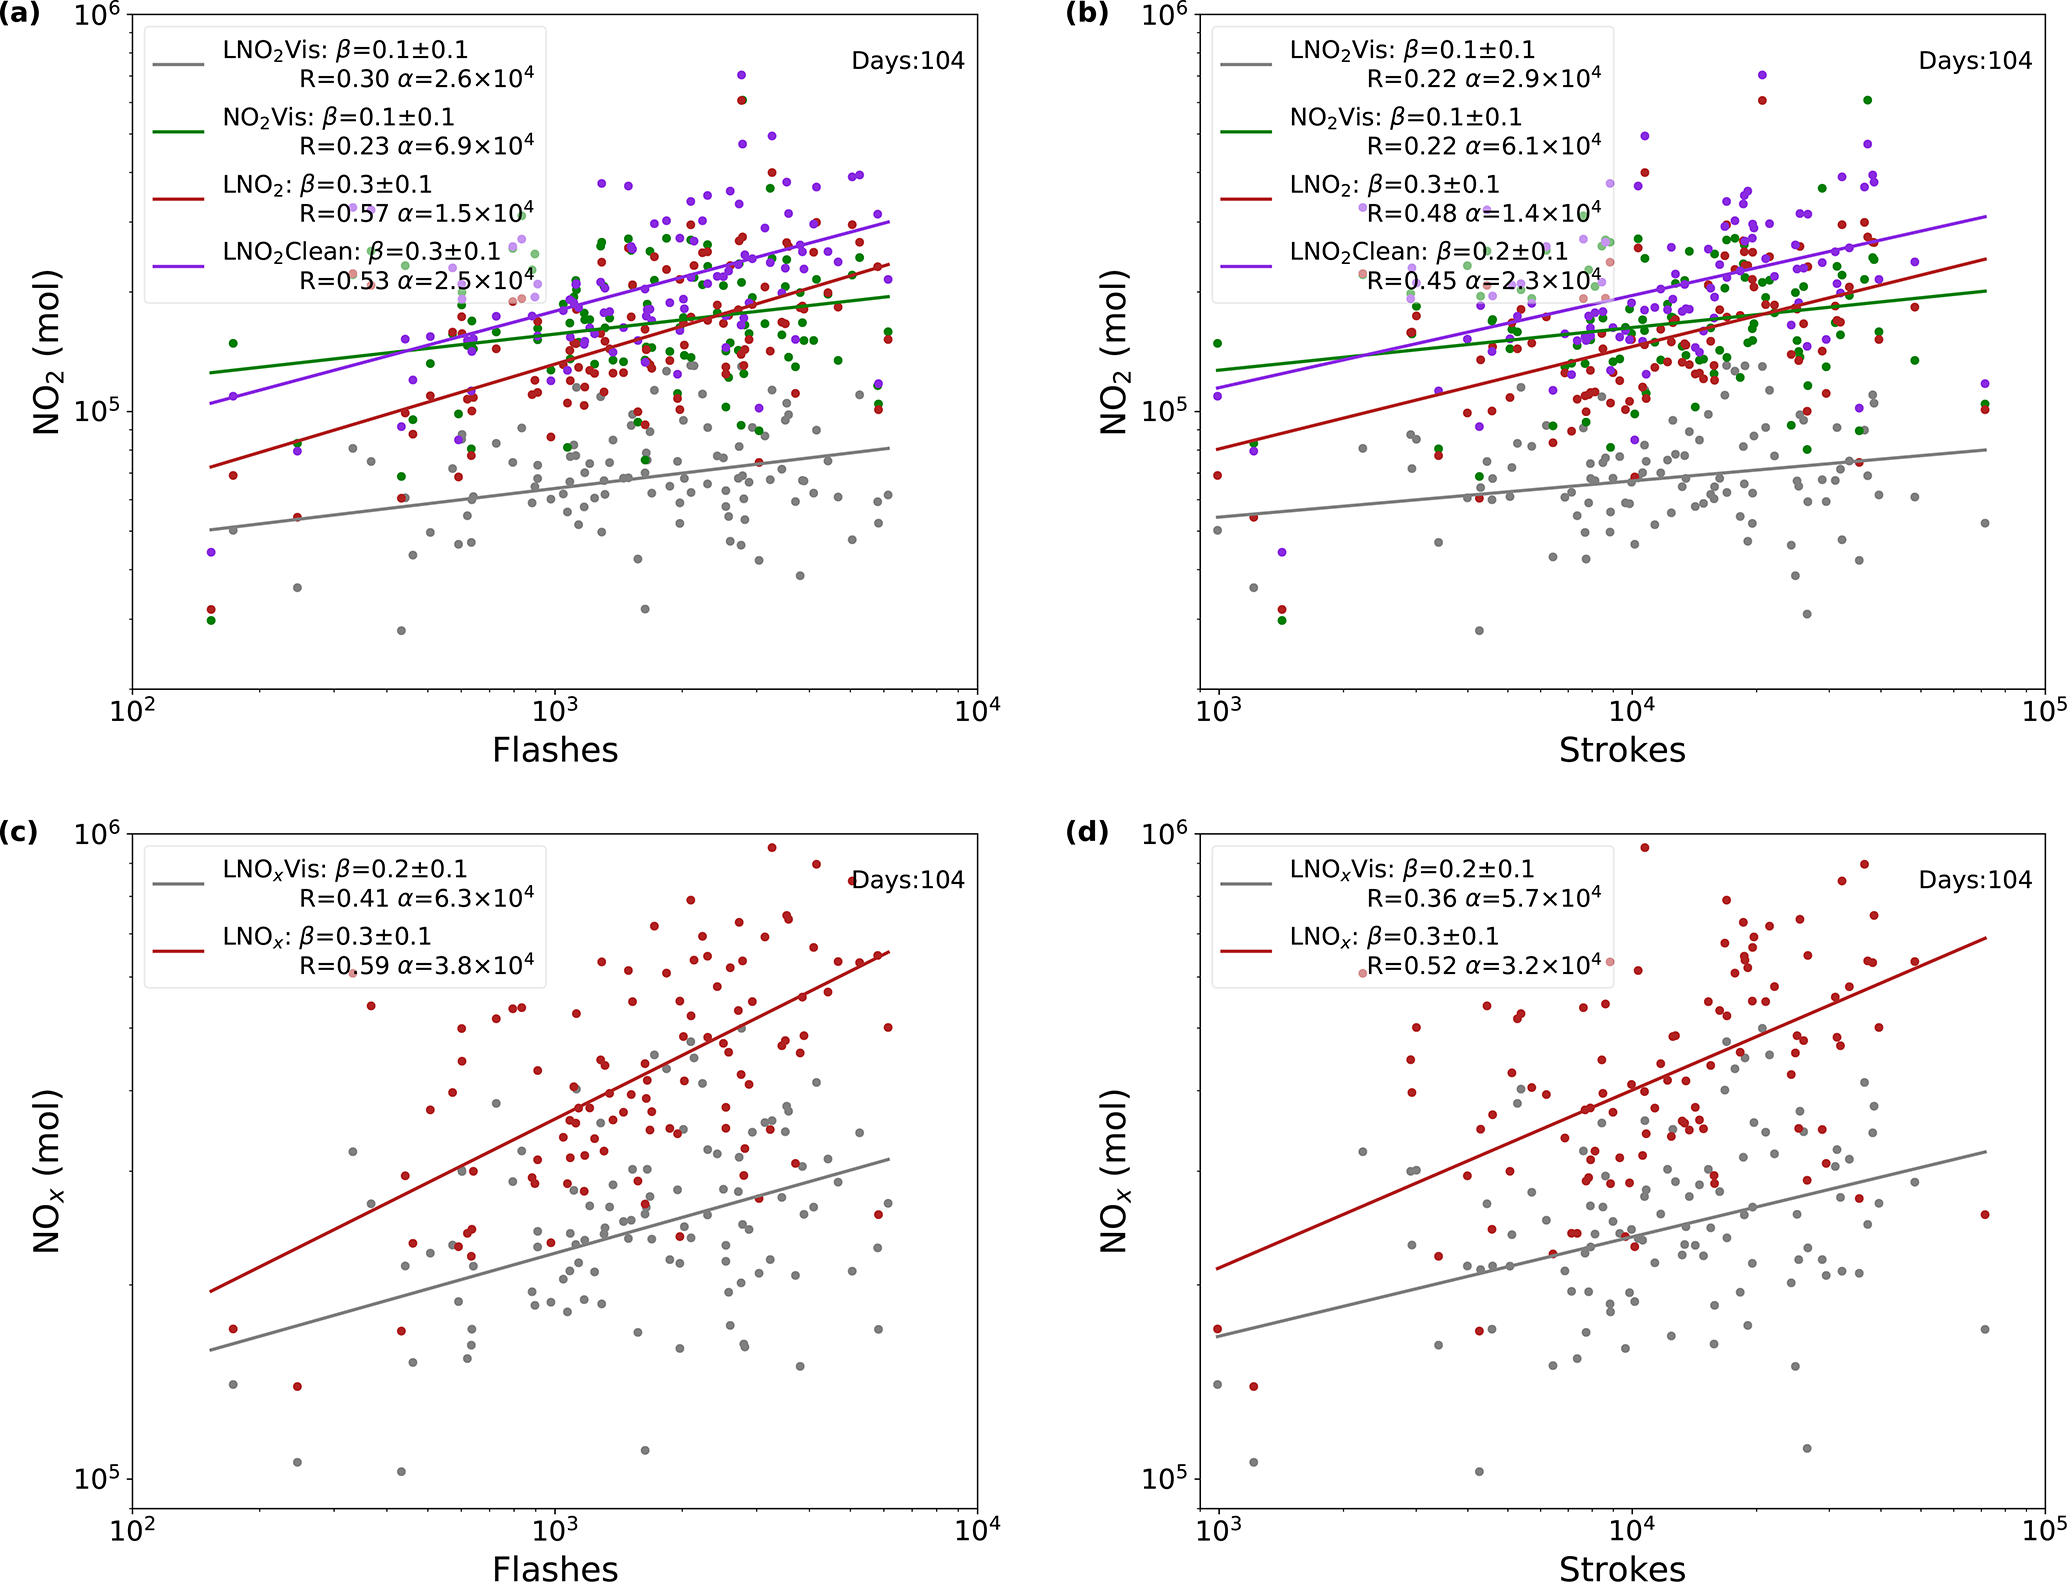
\includegraphics[width=15cm]{amt-2019-372-f14.png}
    \caption{Same as Fig.~\ref{fig:PE_linear_fewerflash} but using log-log axes.}
    \label{fig:PE_power_fewerflash}
\end{figure*}

%fb3
\begin{figure*}[p]
    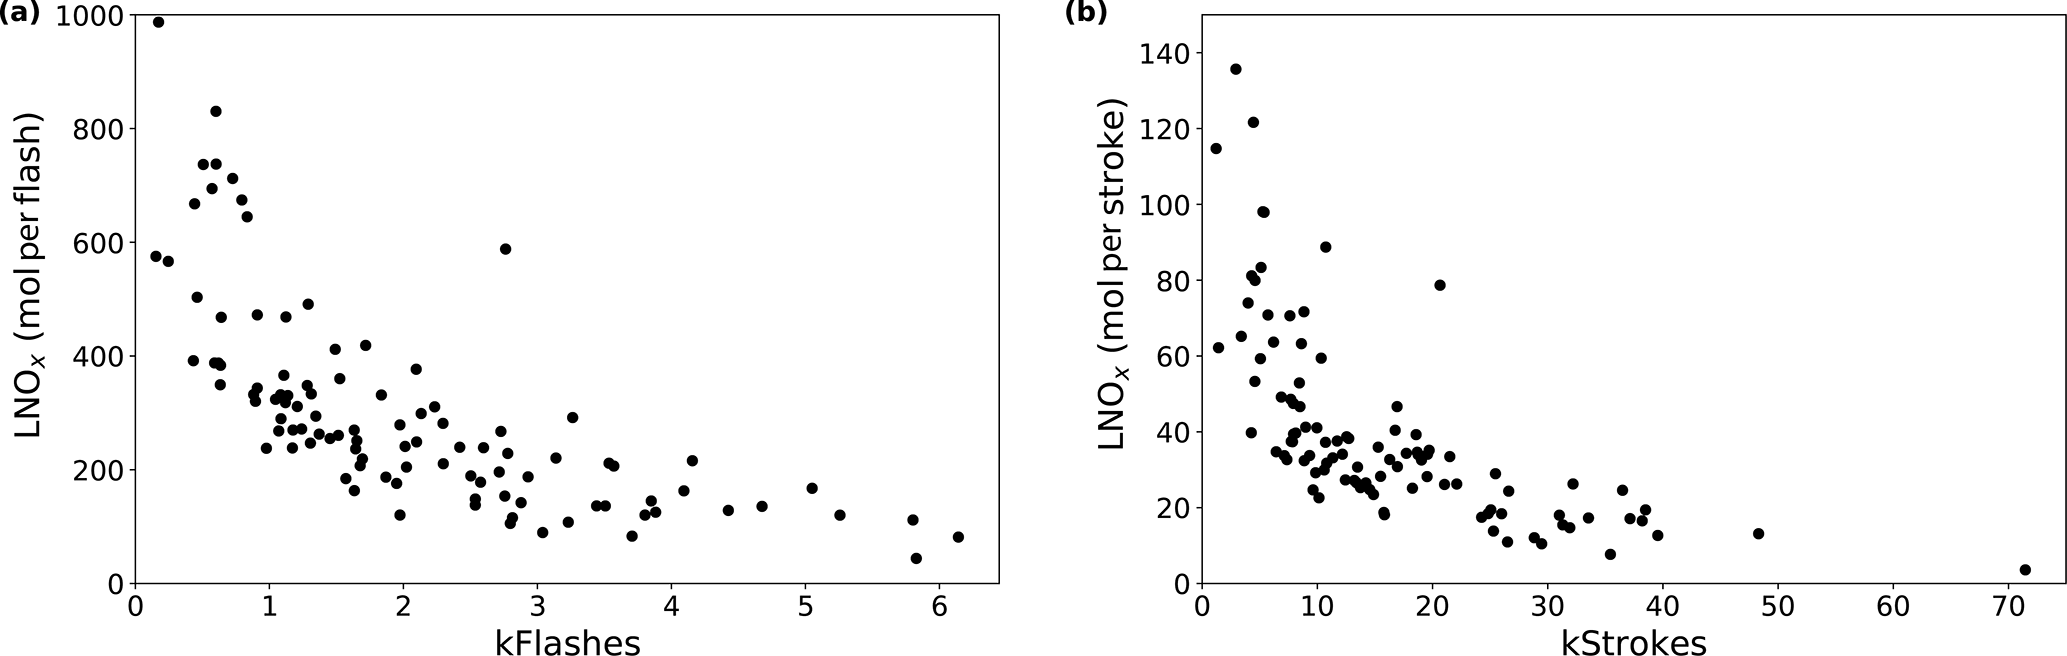
\includegraphics[width=15cm]{amt-2019-372-f15.png}
    \caption{\textbf{(a)}~ Daily L\chem{NO_\mathit{x}} production efficiencies versus ENTLN total flash data, with CRF~$\geq 90$\,{\%} and a flash threshold of one flash per box.
   \textbf{(b)}~Same as \textbf{(a)}~but for strokes.}
    \label{fig:PE_fewerflash}
\end{figure*}


\hack{\clearpage}

\codedataavailability{The retrieval algorithm used in Sect.~\ref{section:AMF} is available at \url{https://github.com/zxdawn/BEHR-LNOx} (last access: 20~March~2020; \doi{10.5281/zenodo.3553426}, \citealp{zhang_xin_2019_3553426}).
The WRF-Chem model output and L\chem{NO_\mathit{x}} product are available upon request to Xin~Zhang (xinzhang1215@gmail.com).
MOZART-4 global model output is available at \url{https://www.acom.ucar.edu/wrf-chem/mozart.shtml} (last access: 20~March~2020).}

\authorcontribution{YY directed the research and RvdA, XZ, and YY designed the research with feedback from the other co-authors;
RvdA and XZ developed the algorithm;
JLL provided guidance and supporting data on the ENTLN data;
XZ performed simulations and analysis with the help of YY, RvdA, QC, XK, SY, JC, CH, and RS;
YY, RvdA, JLL, and XZ interpreted the data and discussed the results.
XZ drafted the manuscript with comments from the co-authors;
JLL, RvdA, and YY edited the manuscript.}

\competinginterests{The authors declare that they have no conflict of interest.}

\begin{acknowledgements}
We acknowledge use of the computational resources provided by the National Supercomputer Centre in Guangzhou (NSCC-GZ).
We thank the University of California Berkeley Satellite Group for the basic BEHR algorithm.
We also thank Earth Networks Company for providing the Earth Networks Total Lightning Network (ENTLN) datasets.
We appreciate the discussions with Joshua~L.~Laughner for BEHR codes and Mary~Barth for the WRF-Chem lightning \chem{NO_\mathit{x}} module.
The authors would also like to thank all anonymous reviewers as well as Kenneth~E.~Pickering, Eric~J.~Bucsela, and Dale~J.~Allen for detailed comments which greatly improved this paper.
Finally, we thank all contributors of Python packages used in this paper \citep{Cartopy,hoyer2017xarray,Hunter.2007,JiaweiZhuang.2019,mckinney2011pandas,plotly.2015,seabold2010statsmodels,vanderWalt.2011,Waskom.2017}.
\end{acknowledgements}

\financialsupport{This research has been supported by the National Natural Science Foundation of China (grant nos. 91644224 and 41705118).}

\reviewstatement{This paper was edited by Steffen Beirle and reviewed by three anonymous referees.}

\begin{thebibliography}{105}


\bibitem[{Acarreta et~al.(2004)Acarreta, de~Haan, and Stammes}]{Acarreta.2004}
Acarreta, J.~R., de~Haan, J.~F., and Stammes, P.: Cloud pressure retrieval
  using the \chem{O_{2}}-\chem{O_{2}} absorption band at 477\,nm,
  J. Geophys. Res., 109, 2165, \doi{10.1029/2003JD003915}, 2004.

\bibitem[{Allen et~al.(2010)Allen, Pickering, Duncan, and Damon}]{Allen.2010}
Allen, D.~J., Pickering, K.~E., Duncan, B.~N., and Damon, M.: Impact of
  lightning NO emissions on North American photochemistry as determined using
  the Global Modeling Initiative (GMI) model, J. Geophys. Res.,
  115, 4711, \doi{10.1029/2010JD014062}, 2010.

\bibitem[{Allen et~al.(2012)Allen, Pickering, Pinder, Henderson, Appel, and
  Prados}]{Allen.2012}
Allen, D. J., Pickering, K. E., Pinder, R. W., Henderson, B. H., Appel, K. W., and Prados, A.: Impact of lightning-NO on eastern United States photochemistry during the summer of 2006 as determined using the CMAQ model, Atmos. Chem. Phys., 12, 1737–1758, \doi{10.5194/acp-12-1737-2012}, 2012.

\bibitem[{Allen et~al.(2019)Allen, Pickering, Bucsela, Krotkov, and
  Holzworth}]{Allen.2019}
Allen, D.~J., Pickering, K.~E., Bucsela, E.~J., Krotkov, N., and Holzworth, R.:
  Lightning \chem{NO_{x}} Production in the Tropics as Determined Using
  OMI \chem{NO_{2}} Retrievals and WWLLN Stroke Data,
  J. Geophys. Res.-Atmos., 124, 13498--13518, \doi{10.1029/2018JD029824}, 2019.

\bibitem[{Banerjee et~al.(2014)Banerjee, Archibald, Maycock, Telford, Abraham,
  Yang, Braesicke, and Pyle}]{Banerjee.2014}
Banerjee, A., Archibald, A. T., Maycock, A. C., Telford, P., Abraham, N. L., Yang, X., Braesicke, P., and Pyle, J. A.: Lightning \chem{NO_x}, a key chemistry–climate interaction: impacts of future climate change and consequences for tropospheric oxidising capacity, Atmos. Chem. Phys., 14, 9871–9881, \doi{10.5194/acp-14-9871-2014}, 2014.

\bibitem[{Barth et~al.(2012)Barth, Lee, Hodzic, Pfister, Skamarock, Worden,
  Wong, and Noone}]{Barth.2012}
Barth, M. C., Lee, J., Hodzic, A., Pfister, G., Skamarock, W. C., Worden, J., Wong, J., and Noone, D.: Thunderstorms and upper troposphere chemistry during the early stages of the 2006 North American Monsoon, Atmos. Chem. Phys., 12, 11003–11026, \doi{10.5194/acp-12-11003-2012}, 2012.

\bibitem[{Beirle et~al.(2004)Beirle, Platt, Wenig, and Wagner}]{Beirle.2004}
Beirle, S., Platt, U., Wenig, M., and Wagner, T.: \chem{NO_\mathit{x}}
  production by lightning estimated with GOME, Adv. Space Res., 34,
  793--797, \doi{10.1016/j.asr.2003.07.069}, 2004.

\bibitem[{Beirle et~al.(2006)Beirle, Spichtinger, Stohl, Cummins, Turner,
  Boccippio, Cooper, Wenig, Grzegorski, Platt, and Wagner}]{Beirle.2006}
Beirle, S., Spichtinger, N., Stohl, A., Cummins, K. L., Turner, T., Boccippio, D., Cooper, O. R., Wenig, M., Grzegorski, M., Platt, U., and Wagner, T.: Estimating the \chem{NO_x} produced by lightning from GOME and NLDN data: a case study in the Gulf of Mexico, Atmos. Chem. Phys., 6, 1075–1089, \doi{10.5194/acp-6-1075-2006}, 2006.

\bibitem[{Beirle et~al.(2009)Beirle, Salzmann, Lawrence, and
  Wagner}]{Beirle.2009}
 Beirle, S., Salzmann, M., Lawrence, M. G., and Wagner, T.: Sensitivity of satellite observations for freshly produced lightning \chem{NO_x}, Atmos. Chem. Phys., 9, 1077–1094, \doi{10.5194/acp-9-1077-2009}, 2009.

\bibitem[{Beirle et~al.(2010)Beirle, Huntrieser, and Wagner}]{Beirle.2010}
Beirle, S., Huntrieser, H., and Wagner, T.: Direct satellite observation of lightning-produced \chem{NO_x}, Atmos. Chem. Phys., 10, 10965–10986, \doi{10.5194/acp-10-10965-2010}, 2010.

\bibitem[{Bela et~al.(2016)Bela, Barth, Toon, Fried, Homeyer, Morrison,
  Cummings, Li, Pickering, Allen, Yang, Wennberg, Crounse, {St. Clair}, Teng,
  O'Sullivan, Huey, Chen, Liu, Blake, Blake, Apel, Hornbrook, Flocke, Campos,
  and Diskin}]{Bela.2016}
Bela, M.~M., Barth, M.~C., Toon, O.~B., Fried, A., Homeyer, C.~R., Morrison,
  H., Cummings, K.~A., Li, Y., Pickering, K.~E., Allen, D.~J., Yang, Q.,
  Wennberg, P.~O., Crounse, J.~D., {St. Clair}, J.~M., Teng, A.~P., O'Sullivan,
  D., Huey, L.~G., Chen, D., Liu, X., Blake, D.~R., Blake, N.~J., Apel, E.~C.,
  Hornbrook, R.~S., Flocke, F., Campos, T., and Diskin, G.: Wet scavenging of
  soluble gases in DC3 deep convective storms using WRF-Chem simulations and
  aircraft observations, J. Geophys. Res.-Atmos., 121,
  4233--4257, \doi{10.1002/2015JD024623}, 2016.

\bibitem[{Boersma et~al.(2005)Boersma, Eskes, Meijer, and
  Kelder}]{Boersma.2005}
Boersma, K. F., Eskes, H. J., Meijer, E. W., and Kelder, H. M.: Estimates of lightning \chem{NO_x} production from GOME satellite observations, Atmos. Chem. Phys., 5, 2311–2331, \doi{10.5194/acp-5-2311-2005}, 2005.

\bibitem[{Boersma et~al.(2018)Boersma, Eskes, Richter, de~Smedt, Lorente,
  Beirle, {van Geffen}, Zara, Peters, {van Roozendael}, Wagner, d.~Maasakkers,
  {van der A}, Nightingale, de~Rudder, Irie, Pinardi, Lambert, and
  Compernolle}]{Boersma.2018}
 Boersma, K. F., Eskes, H. J., Richter, A., De Smedt, I., Lorente, A., Beirle, S., van Geffen, J. H. G. M., Zara, M., Peters, E., Van Roozendael, M., Wagner, T., Maasakkers, J. D., van der A, R. J., Nightingale, J., De Rudder, A., Irie, H., Pinardi, G., Lambert, J.-C., and Compernolle, S. C.: Improving algorithms and uncertainty estimates for satellite \chem{NO_2} retrievals: results from the quality assurance for the essential climate variables (QA4ECV) project, Atmos. Meas. Tech., 11, 6651--6678, \doi{10.5194/amt-11-6651-2018}, 2018.

\bibitem[{Bovensmann et~al.(1999)Bovensmann, Burrows, Buchwitz, Frerick, Noël,
  Rozanov, Chance, and Goede}]{Bovensmann.1999}
Bovensmann, H., Burrows, J.~P., Buchwitz, M., Frerick, J., Noël, S., Rozanov,
  V.~V., Chance, K.~V., and Goede, A. P.~H.: SCIAMACHY: Mission Objectives and
  Measurement Modes, J. Atmos. Sci., 56, 127--150,
  \doi{10.1175/1520-0469(1999)056<0127:SMOAMM>2.0.CO;2}, 1999.

\bibitem[{Browne et~al.(2014)Browne, Wooldridge, Min, and Cohen}]{Browne.2014}
Browne, E. C., Wooldridge, P. J., Min, K.-E., and Cohen, R. C.: On the role of monoterpene chemistry in the remote continental boundary layer, Atmos. Chem. Phys., 14, 1225–1238, \doi{10.5194/acp-14-1225-2014}, 2014.

\bibitem[{Bucsela et~al.(2010)Bucsela, Pickering, Huntemann, Cohen, Perring,
  Gleason, Blakeslee, Albrecht, Holzworth, Cipriani, Vargas-Navarro,
  Mora-Segura, Pacheco-Hernández, and Laporte-Molina}]{Bucsela.2010}
Bucsela, E.~J., Pickering, K.~E., Huntemann, T.~L., Cohen, R.~C., Perring, A.,
  Gleason, J.~F., Blakeslee, R.~J., Albrecht, R.~I., Holzworth, R., Cipriani,
  J.~P., Vargas-Navarro, D., Mora-Segura, I., Pacheco-Hernández, A., and
  Laporte-Molina, S.: Lightning-generated \chem{NO_{x}} seen by the Ozone
  Monitoring Instrument during NASA's Tropical Composition, Cloud and Climate
  Coupling Experiment (TC$_{4}$), J. Geophys. Res.,
  115, 793, \doi{10.1029/2009JD013118}, 2010.

\bibitem[{Bucsela et~al.(2013)Bucsela, Krotkov, Celarier, Lamsal, Swartz,
  Bhartia, Boersma, Veefkind, Gleason, and Pickering}]{Bucsela.2013}
 Bucsela, E. J., Krotkov, N. A., Celarier, E. A., Lamsal, L. N., Swartz, W. H., Bhartia, P. K., Boersma, K. F., Veefkind, J. P., Gleason, J. F., and Pickering, K. E.: A new stratospheric and tropospheric \chem{NO_2} retrieval algorithm for nadir-viewing satellite instruments: applications to OMI, Atmos. Meas. Tech., 6, 2607–2626, \doi{10.5194/amt-6-2607-2013}, 2013.

\bibitem[{Bucsela et~al.(2019)Bucsela, Pickering, Allen, Holzworth, and
  Krotkov}]{Bucsela.2019}
Bucsela, E.~J., Pickering, K.~E., Allen, D.~J., Holzworth, R., and Krotkov,
  N.~A.: Midlatitude lightning \chem{NO_{x}} production efficiency
  inferred from OMI and WWLLN data, J. Geophys. Res.-Atmos.,  124, 13475--13497, \doi{10.1029/2019JD030561}, 2019.

\bibitem[{Burrows et~al.(1999)Burrows, Weber, Buchwitz, Rozanov,
  Ladstätter-Weißenmayer, Richter, DeBeek, Hoogen, Bramstedt, Eichmann,
  Eisinger, and Perner}]{Burrows.1999}
Burrows, J.~P., Weber, M., Buchwitz, M., Rozanov, V., Ladstätter-Weißenmayer,
  A., Richter, A., DeBeek, R., Hoogen, R., Bramstedt, K., Eichmann, K.-U.,
  Eisinger, M., and Perner, D.: The Global Ozone Monitoring Experiment (GOME):
  Mission Concept and First Scientific Results, J. Atmos. Sci., 56, 151--175,
  \doi{10.1175/1520-0469(1999)056<0151:TGOMEG>2.0.CO;2}, 1999.

\bibitem[{Callies et~al.(2000)Callies, Corpaccioli, Eisinger, Hahne, and
  Lefebvre}]{Callies.2000}
Callies, J., Corpaccioli, E., Eisinger, M., Hahne, A., and Lefebvre, A.:
  GOME-2-Metop's second-generation sensor for operational ozone monitoring, ESA
  Bulletin, 102, 28--36, 2000.

\bibitem[{Carey et~al.(2016)Carey, Koshak, Peterson, and
  Mecikalski}]{Carey.2016}
Carey, L.~D., Koshak, W., Peterson, H., and Mecikalski, R.~M.: The kinematic
  and microphysical control of lightning rate, extent, and \chem{NO_x} production,
  J. Geophys. Res.-Atmos., 121, 7975--7989,
  \doi{10.1002/2015JD024703}, 2016.

\bibitem[{Choi et~al.(2014)Choi, Joiner, Choi, Duncan, Vasilkov, Krotkov, and
  Bucsela}]{Choi.2014}
Choi, S., Joiner, J., Choi, Y., Duncan, B. N., Vasilkov, A., Krotkov, N., and Bucsela, E.: First estimates of global free-tropospheric \chem{NO_2} abundances derived using a cloud-slicing technique applied to satellite observations from the Aura Ozone Monitoring Instrument (OMI), Atmos. Chem. Phys., 14, 10565–10588, \doi{10.5194/acp-14-10565-2014}, 2014.

\bibitem[{Clark et~al.(2017)Clark, Ward, and Mahowald}]{Clark.2017}
Clark, S.~K., Ward, D.~S., and Mahowald, N.~M.: Parameterization-based
  uncertainty in future lightning flash density,
  Geophys. Res. Lett.,
  44, 2893--2901, \doi{10.1002/2017GL073017}, 2017.

\bibitem[{Davis et~al.(2019)Davis, Rutledge, and Fuchs}]{Davis.2019}
Davis, T.~C., Rutledge, S.~A., and Fuchs, B.~R.: Lightning location, \chem{NO_x}
  production, and transport by anomalous and normal polarity thunderstorms,
  J. Geophys. Res.-Atmos., 124, 8722--8742, \doi{10.1029/2018JD029979},
  2019.

\bibitem[{DeCaria et~al.(2000)DeCaria, Pickering, Stenchikov, Scala, Stith,
  Dye, Ridley, and Laroche}]{DeCaria.2000}
DeCaria, A.~J., Pickering, K.~E., Stenchikov, G.~L., Scala, J.~R., Stith,
  J.~L., Dye, J.~E., Ridley, B.~A., and Laroche, P.: A cloud-scale model study
  of lightning-generated \chem{NO_{x}} in an individual thunderstorm
  during STERAO-A, J. Geophys. Res., 105, 11601--11616,
  \doi{10.1029/2000JD900033}, 2000.

\bibitem[{DeCaria et~al.(2005)DeCaria, Pickering, Stenchikov, and
  Ott}]{DeCaria.2005}
DeCaria, A.~J., Pickering, K.~E., Stenchikov, G.~L., and Ott, L.~E.:
  Lightning-generated \chem{NO_{x}} and its impact on tropospheric ozone
  production: A three-dimensional modeling study of a Stratosphere-Troposphere
  Experiment: Radiation, Aerosols and Ozone (STERAO-A) thunderstorm,
  J. Geophys. Res., 110,  D14303, \doi{10.1029/2004JD005556}, 2005.

\bibitem[{Dobber et~al.(2008)Dobber, Kleipool, Dirksen, Levelt, Jaross, Taylor,
  Kelly, Flynn, Leppelmeier, and Rozemeijer}]{Dobber.2008}
Dobber, M., Kleipool, Q., Dirksen, R., Levelt, P., Jaross, G., Taylor, S.,
  Kelly, T., Flynn, L., Leppelmeier, G., and Rozemeijer, N.: Validation of
  Ozone Monitoring Instrument level 1b data products, J. Geophys. Res., 113, 5224, \doi{10.1029/2007JD008665}, 2008.

\bibitem[{Emmons et~al.(2010)Emmons, Walters, Hess, Lamarque, Pfister,
  Fillmore, Granier, Guenther, Kinnison, Laepple, Orlando, Tie, Tyndall,
  Wiedinmyer, Baughcum, and Kloster}]{Emmons.2010}
Emmons, L. K., Walters, S., Hess, P. G., Lamarque, J.-F., Pfister, G. G., Fillmore, D., Granier, C., Guenther, A., Kinnison, D., Laepple, T., Orlando, J., Tie, X., Tyndall, G., Wiedinmyer, C., Baughcum, S. L., and Kloster, S.: Description and evaluation of the Model for Ozone and Related chemical Tracers, version 4 (MOZART-4), Geosci. Model Dev., 3, 43–67, \doi{10.5194/gmd-3-43-2010}, 2010.

\bibitem[{EPA(2015)}]{us20152011}
EPA: 2011 National Emissions Inventory, version 2--Technical support
  document, US Environmental Protection Agency, Office of Air Quality Planning
  and Standards, available at: \url{https://www.epa.gov/air-emissions-inventories/2011-national-emissions-inventory-nei-technical-support-document} (last access: 3~April~2020), 2015.

\bibitem[{EPA and OAR(2015)}]{EPA.2015}
EPA and OAR: Air Pollutant Emissions Trends Data $|$ US EPA,
available at: \url{https://www.epa.gov/air-emissions-inventories/air-pollutant-emissions-trends-data} (last access: 3~April~2020),
  2015.

\bibitem[{Finney et~al.(2016)Finney, Doherty, Wild, Young, and
  Butler}]{Finney.2016}
Finney, D.~L., Doherty, R.~M., Wild, O., Young, P.~J., and Butler, A.: Response
  of lightning \chem{NO_x} emissions and ozone production to climate change: Insights
  from the Atmospheric Chemistry and Climate Model Intercomparison Project,
  Geophys. Res. Lett., 43, 5492--5500, \doi{10.1002/2016GL068825},
  2016.

\bibitem[{Finney et~al.(2018)Finney, Doherty, Wild, Stevenson, MacKenzie, and
  Blyth}]{Finney.2018}
Finney, D.~L., Doherty, R.~M., Wild, O., Stevenson, D.~S., MacKenzie, I.~A.,
  and Blyth, A.~M.: A projected decrease in lightning under climate change,
  Nat. Clim. Change, 8, 210--213, \doi{10.1038/s41558-018-0072-6}, 2018.

\bibitem[{Fried et~al.(2016)Fried, Barth, Bela, Weibring, Richter, Walega, Li,
  Pickering, Apel, Hornbrook, Hills, Riemer, Blake, Blake, Schroeder, Luo,
  Crawford, Olson, Rutledge, Betten, Biggerstaff, Diskin, Sachse, Campos,
  Flocke, Weinheimer, Cantrell, Pollack, Peischl, Froyd, Wisthaler, Mikoviny,
  and Woods}]{Fried.2016}
Fried, A., Barth, M.~C., Bela, M., Weibring, P., Richter, D., Walega, J., Li,
  Y., Pickering, K., Apel, E., Hornbrook, R., Hills, A., Riemer, D.~D., Blake,
  N., Blake, D.~R., Schroeder, J.~R., Luo, Z.~J., Crawford, J.~H., Olson, J.,
  Rutledge, S., Betten, D., Biggerstaff, M.~I., Diskin, G.~S., Sachse, G.,
  Campos, T., Flocke, F., Weinheimer, A., Cantrell, C., Pollack, I., Peischl,
  J., Froyd, K., Wisthaler, A., Mikoviny, T., and Woods, S.: Convective
  transport of formaldehyde to the upper troposphere and lower stratosphere and
  associated scavenging in thunderstorms over the central United States during
  the 2012 DC3 study, J. Geophys. Res.-Atmos., 121,
  7430--7460, \doi{10.1002/2015JD024477}, 2016.

\bibitem[{Fuchs and Rutledge(2018)}]{Fuchs.2018}
Fuchs, B.~R. and Rutledge, S.~A.: Investigation of Lightning Flash Locations in
  Isolated Convection Using LMA Observations, J. Geophys. Res.-Atmos., 123, 6158--6174, \doi{10.1002/2017JD027569}, 2018.

\bibitem[{Goliff et~al.(2013)Goliff, Stockwell, and Lawson}]{Goliff.2013}
Goliff, W.~S., Stockwell, W.~R., and Lawson, C.~V.: The regional atmospheric
  chemistry mechanism, version 2, Atmos. Environ., 68, 174--185,
  \doi{10.1016/j.atmosenv.2012.11.038}, 2013.

\bibitem[{Grell et~al.(2005)Grell, Peckham, Schmitz, McKeen, Frost, Skamarock,
  and Eder}]{Grell.2005}
Grell, G.~A., Peckham, S.~E., Schmitz, R., McKeen, S.~A., Frost, G., Skamarock,
  W.~C., and Eder, B.: Fully coupled ``online'' chemistry within the WRF
  model, Atmos. Environ., 39, 6957--6975,
  \doi{10.1016/j.atmosenv.2005.04.027}, 2005.

\bibitem[{Griffin et~al.(2019)Griffin, Zhao, McLinden, Boersma, Bourassa,
  Dammers, Degenstein, Eskes, Fehr, Fioletov, Hayden, Kharol, Li, Makar,
  Martin, Mihele, Mittermeier, Krotkov, Sneep, Lamsal, Linden, {van Geffen},
  Veefkind, and Wolde}]{Griffin.2019}
Griffin, D., Zhao, X., McLinden, C.~A., Boersma, F., Bourassa, A., Dammers, E.,
  Degenstein, D., Eskes, H., Fehr, L., Fioletov, V., Hayden, K., Kharol, S.~K.,
  Li, S.-M., Makar, P., Martin, R.~V., Mihele, C., Mittermeier, R.~L., Krotkov,
  N., Sneep, M., Lamsal, L.~N., Linden, M.~T., {van Geffen}, J., Veefkind, P.,
  and Wolde, M.: High-Resolution Mapping of Nitrogen Dioxide With TROPOMI:
  First Results and Validation Over the Canadian Oil Sands, Geophys. Res. Lett., 46, 1049--1060, \doi{10.1029/2018GL081095}, 2019.

\bibitem[{Guenther et~al.(2006)Guenther, Karl, Harley, Wiedinmyer, Palmer, and
  Geron}]{Guenther.2006}
Guenther, A., Karl, T., Harley, P., Wiedinmyer, C., Palmer, P. I., and Geron, C.: Estimates of global terrestrial isoprene emissions using MEGAN (Model of Emissions of Gases and Aerosols from Nature), Atmos. Chem. Phys., 6, 3181–3210, \doi{10.5194/acp-6-3181-2006}, 2006.

\bibitem[{Hauglustaine et~al.(2001)Hauglustaine, Emmons, Newchurch, Brasseur,
  Takao, Matsubara, Johnson, Ridley, Stith, and Dye}]{Hauglustaine.2001}
Hauglustaine, D., Emmons, L., Newchurch, M., Brasseur, G., Takao, T.,
  Matsubara, K., Johnson, J., Ridley, B., Stith, J., and Dye, J.: On the Role
  of Lightning NO{x} in the Formation of Tropospheric Ozone
  Plumes: A Global Model Perspective, J. Atmos. Chem., 38,
  277--294, \doi{10.1023/A:1006452309388}, 2001.

\bibitem[{Hoyer and Hamman(2017)}]{hoyer2017xarray}
Hoyer, S. and Hamman, J.: xarray: {N-D} labeled arrays and datasets in
  {Python}, Journal of Open Research Software, 5, 10, \doi{10.5334/jors.148},
   2017.

\bibitem[{Hunter(2007)}]{Hunter.2007}
Hunter, J.~D.: Matplotlib: A 2D Graphics Environment,
Comput. Sci. Eng., 9, 90--95, \doi{10.1109/MCSE.2007.55}, 2007.

\bibitem[{Inc.(2015)}]{plotly.2015}
Inc.: Collaborative data science, available at: \url{https://plot.ly} (last access: 3~April~2020), 2015.



\bibitem[{Joiner et~al.(2012)Joiner, Vasilkov, Gupta, Bhartia, Veefkind, Sneep,
  de~Haan, Polonsky, and Spurr}]{Joiner.2012}
Joiner, J., Vasilkov, A. P., Gupta, P., Bhartia, P. K., Veefkind, P., Sneep, M., de Haan, J., Polonsky, I., and Spurr, R.: Fast simulators for satellite cloud optical centroid pressure retrievals; evaluation of OMI cloud retrievals, Atmos. Meas. Tech., 5, 529–545, \doi{10.5194/amt-5-529-2012}, 2012.

\bibitem[{KNMI(2012)}]{KNMI.2020}
KNMI: Background information about the Row Anomaly in OMI,
 available at: \url{http://projects.knmi.nl/omi/research/product/rowanomaly-background.php},
  (last access: 3~April~2020), 2012.

\bibitem[{Krause et~al.(2014)Krause, Kloster, Wilkenskjeld, and
  Paeth}]{Krause.2014}
Krause, A., Kloster, S., Wilkenskjeld, S., and Paeth, H.: The sensitivity of
  global wildfires to simulated past, present, and future lightning frequency,
  J. Geophys. Res.-Biogeo., 119, 312--322,
  \doi{10.1002/2013JG002502}, 2014.

\bibitem[{Krotkov et~al.(2017)Krotkov, Lamsal, Celarier, Swartz, Marchenko,
  Bucsela, Chan, Wenig, and Zara}]{Krotkov.2017}
Krotkov, N. A., Lamsal, L. N., Celarier, E. A., Swartz, W. H., Marchenko, S. V., Bucsela, E. J., Chan, K. L., Wenig, M., and Zara, M.: The version 3 OMI \chem{NO_2} standard product, Atmos. Meas. Tech., 10, 3133–3149, \doi{10.5194/amt-10-3133-2017}, 2017.

\bibitem[{Kuhlmann et~al.(2014)Kuhlmann, Hartl, Cheung, Lam, and
  Wenig}]{Kuhlmann.2014}
 Kuhlmann, G., Hartl, A., Cheung, H. M., Lam, Y. F., and Wenig, M. O.: A novel gridding algorithm to create regional trace gas maps from satellite observations, Atmos. Meas. Tech., 7, 451–467, \doi{10.5194/amt-7-451-2014}, 2014.

\bibitem[{Lapierre et~al.(2020)Lapierre, Laughner, Geddes, Koshak, Cohen, and
  Pusede}]{Lapierre.2020}
Lapierre, J.~L., Laughner, J.~L., Geddes, J.~A., Koshak, W., Cohen, R.~C., and
  Pusede, S.~E.: Observing U.S. regional variability in lightning
  \chem{NO_{2}} production rates, J. Geophys. Res.-Atmos., 125, e2019JD031362, \doi{10.1029/2019JD031362}, 2020.

\bibitem[{Laughner and Cohen(2017)}]{Laughner.2017}
Laughner, J. L. and Cohen, R. C.: Quantification of the effect of modeled lightning \chem{NO_2} on UV–visible air mass factors, Atmos. Meas. Tech., 10, 4403–4419, \doi{10.5194/amt-10-4403-2017}, 2017.

\bibitem[{Laughner et~al.(2018)Laughner, Zhu, and
  Cohen}]{Laughner.2018}
 Laughner, J. L., Zhu, Q., and Cohen, R. C.: The Berkeley High Resolution Tropospheric \chem{NO_2} product, Earth Syst. Sci. Data, 10, 2069–2095, \doi{10.5194/essd-10-2069-2018},  2018.

\bibitem[{Laughner et~al.(2019)Laughner, Zhu, and
  Cohen}]{Laughner.2019}
Laughner, J. L., Zhu, Q., and Cohen, R. C.: Evaluation of version 3.0B of the BEHR OMI \chem{NO_2} product, Atmos. Meas. Tech., 12, 129–146, \doi{10.5194/amt-12-129-2019}, 2019.



\bibitem[{Levelt et~al.(2006)Levelt, {van den Oord}, Dobber, Malkki, Visser,
  Vries, Stammes, Lundell, and Saari}]{Levelt.2006}
Levelt, P.~F., {van den Oord}, G., Dobber, M.~R., Malkki, A., Visser, H.,
  Vries, J.~D., Stammes, P., Lundell, J., and Saari, H.: The ozone monitoring
  instrument, IEEE T. Geosci. Remote, 44,
  1093--1101, \doi{10.1109/TGRS.2006.872333}, 2006.

\bibitem[{Levelt et~al.(2018)Levelt, Joiner, Tamminen, Veefkind, Bhartia,
  {Stein Zweers}, Duncan, Streets, Eskes, {van der A}, McLinden, Fioletov,
  Carn, de~Laat, DeLand, Marchenko, McPeters, Ziemke, Fu, Liu, Pickering,
  Apituley, {González Abad}, Arola, Boersma, {Chan Miller}, Chance, de~Graaf,
  Hakkarainen, Hassinen, Ialongo, Kleipool, Krotkov, Li, Lamsal, Newman,
  Nowlan, Suleiman, Tilstra, Torres, Wang, and Wargan}]{Levelt.2018}
Levelt, P. F., Joiner, J., Tamminen, J., Veefkind, J. P., Bhartia, P. K., Stein Zweers, D. C., Duncan, B. N., Streets, D. G., Eskes, H., van der A, R., McLinden, C., Fioletov, V., Carn, S., de Laat, J., DeLand, M., Marchenko, S., McPeters, R., Ziemke, J., Fu, D., Liu, X., Pickering, K., Apituley, A., González Abad, G., Arola, A., Boersma, F., Chan Miller, C., Chance, K., de Graaf, M., Hakkarainen, J., Hassinen, S., Ialongo, I., Kleipool, Q., Krotkov, N., Li, C., Lamsal, L., Newman, P., Nowlan, C., Suleiman, R., Tilstra, L. G., Torres, O., Wang, H., and Wargan, K.: The Ozone Monitoring Instrument: overview of 14 years in space, Atmos. Chem. Phys., 18, 5699–5745, \doi{10.5194/acp-18-5699-2018}, 2018.

\bibitem[{Li et~al.(2017)Li, Pickering, Allen, Barth, Bela, Cummings, Carey,
  Mecikalski, Fierro, Campos, Weinheimer, Diskin, and Biggerstaff}]{Li.2017}
Li, Y., Pickering, K.~E., Allen, D.~J., Barth, M.~C., Bela, M.~M., Cummings,
  K.~A., Carey, L.~D., Mecikalski, R.~M., Fierro, A.~O., Campos, T.~L.,
  Weinheimer, A.~J., Diskin, G.~S., and Biggerstaff, M.~I.: Evaluation of deep
  convective transport in storms from different convective regimes during the
  DC3 field campaign using WRF-Chem with lightning data assimilation, J. Geophys. Res.-Atmos., 122, 7140--7163,
  \doi{10.1002/2017JD026461}, 2017.

\bibitem[{Li et~al.(2018)Li, Pickering, Barth, Bela, Cummings, and
  Allen}]{Li.2018}
Li, Y., Pickering, K.~E., Barth, M.~C., Bela, M.~M., Cummings, K.~A., and
  Allen, D.~J.: Evaluation of Parameterized Convective Transport of Trace Gases
  in Simulation of Storms Observed During the DC3 Field Campaign, J. Geophys. Res.-Atmos., 123, 11238--11261,
  \doi{10.1029/2018JD028779}, 2018.

\bibitem[{Luo et~al.(2017)Luo, Wang, and Koshak}]{Luo.2017}
Luo, C., Wang, Y., and Koshak, W.~J.: Development of a self-consistent
  lightning \chem{NO_\mathit{x}} simulation in large-scale 3-D models, J. Geophys. Res.-Atmos., 122, 3141--3154, \doi{10.1002/2016JD026225}, 2017.

\bibitem[{Marais et~al.(2018)Marais, Jacob, Choi, Joiner, Belmonte-Rivas,
  Cohen, Beirle, Murray, Schiferl, Shah, and Jaeglé}]{Marais.2018}
Marais, E. A., Jacob, D. J., Choi, S., Joiner, J., Belmonte-Rivas, M., Cohen, R. C., Beirle, S., Murray, L. T., Schiferl, L. D., Shah, V., and Jaeglé, L.: Nitrogen oxides in the global upper troposphere: interpreting cloud-sliced \chem{NO_2} observations from the OMI satellite instrument, Atmos. Chem. Phys., 18, 17017–17027, \doi{10.5194/acp-18-17017-2018}, 2018.


\bibitem[{Martin et~al.(2007)Martin, Sauvage, Folkins, Sioris, Boone, Bernath,
  and Ziemke}]{Martin.2007}
Martin, R.~V., Sauvage, B., Folkins, I., Sioris, C.~E., Boone, C., Bernath, P.,
  and Ziemke, J.: Space-based constraints on the production of nitric oxide by
  lightning, J. Geophys. Res., 112, 1479,
  \doi{10.1029/2006JD007831}, 2007.

\bibitem[{McKinney(2011)}]{mckinney2011pandas}
McKinney, W.: pandas: a foundational Python library for data analysis and
  statistics, Python for High Performance and Scientific Computing, 14, 2011.

\bibitem[{Mecikalski and Carey(2017)}]{Mecikalski.2017}
Mecikalski, R.~M. and Carey, L.~D.: Lightning characteristics relative to
  radar, altitude and temperature for a multicell, MCS and supercell over
  northern Alabama, Atmos. Res., 191, 128--140,
  \doi{10.1016/j.atmosres.2017.03.001},
  2017.

\bibitem[{{Met Office}(2010--2015)}]{Cartopy}
{Met Office}: Cartopy: a cartographic python library with a matplotlib
  interface, Exeter, Devon, available at: \url{http://scitools.org.uk/cartopy} (last access: 3~April~2020),
  2010--2015.

\bibitem[{Min et~al.(2017)Min, Wu, Li, Liu, Xu, Wu, Chen, Wang, Sun, Qin, Wang,
  Li, Zheng, Cao, and Dong}]{Min.2017}
Min, M., Wu, C., Li, C., Liu, H., Xu, N., Wu, X., Chen, L., Wang, F., Sun, F.,
  Qin, D., Wang, X., Li, B., Zheng, Z., Cao, G., and Dong, L.: Developing the
  science product algorithm testbed for Chinese next-generation geostationary
  meteorological satellites: Fengyun-4 series, J. Meteorol.
  Res., 31, 708--719, \doi{10.1007/s13351-017-6161-z}, 2017.

\bibitem[{Myhre et~al.(2013)Myhre, Shindell, Bréon, Collins, Fuglestvedt,
  Huang, Koch, Lamarque, Lee, and Mendoza}]{Myhre.2013}
Myhre, G., Shindell, D., Bréon, F.~M., Collins, W., Fuglestvedt, J., Huang,
  J., Koch, D., Lamarque, J.~F., Lee, D., and Mendoza, B.: Climate change 2013:
  the physical science basis. Contribution of Working Group I to the Fifth
  Assessment Report of the Intergovernmental Panel on Climate Change, edited by:
  Tignor, M., Allen, S. K., Boschung, J., Nauels, A., Xia, Y., Bex, V., and
  Midgley, P. M., Cambridge University Press Cambridge, UK and New
  York, NY, USA, 2013.

\bibitem[{Nault et~al.(2016)Nault, Garland, Wooldridge, Brune, Campuzano-Jost,
  Crounse, Day, Dibb, Hall, Huey, Jimenez, Liu, Mao, Mikoviny, Peischl,
  Pollack, Ren, Ryerson, Scheuer, Ullmann, Wennberg, Wisthaler, Zhang, and
  Cohen}]{Nault.2016}
Nault, B.~A., Garland, C., Wooldridge, P.~J., Brune, W.~H., Campuzano-Jost, P.,
  Crounse, J.~D., Day, D.~A., Dibb, J., Hall, S.~R., Huey, L.~G., Jimenez,
  J.~L., Liu, X., Mao, J., Mikoviny, T., Peischl, J., Pollack, I.~B., Ren, X.,
  Ryerson, T.~B., Scheuer, E., Ullmann, K., Wennberg, P.~O., Wisthaler, A.,
  Zhang, L., and Cohen, R.~C.: Observational Constraints on the Oxidation of NO
  x in the Upper Troposphere, J. Phys. Chem. A, 120,
  1468--1478, \doi{10.1021/acs.jpca.5b07824}, 2016.

\bibitem[{Nault et~al.(2017)Nault, Laughner, Wooldridge, Crounse, Dibb, Diskin,
  Peischl, Podolske, Pollack, Ryerson, Scheuer, Wennberg, and
  Cohen}]{Nault.2017}
Nault, B.~A., Laughner, J.~L., Wooldridge, P.~J., Crounse, J.~D., Dibb, J.,
  Diskin, G., Peischl, J., Podolske, J.~R., Pollack, I.~B., Ryerson, T.~B.,
  Scheuer, E., Wennberg, P.~O., and Cohen, R.~C.: Lightning \chem{NO_\mathit{x}}
  Emissions: Reconciling Measured and Modeled Estimates With Updated
 \chem{NO_\mathit{x}} Chemistry, Geophys. Res. Lett., 44, 9479--9488,
  \doi{10.1002/2017GL074436}, 2017.

\bibitem[{Ott et~al.(2007)Ott, Pickering, Stenchikov, Huntrieser, and
  Schumann}]{Ott.2007}
Ott, L.~E., Pickering, K.~E., Stenchikov, G.~L., Huntrieser, H., and Schumann,
  U.: Effects of lightning NO x production during the 21 July European
  Lightning Nitrogen Oxides Project storm studied with a three-dimensional
  cloud-scale chemical transport model, J. Geophys. Res., 112,
 D05307, \doi{10.1029/2006JD007365}, 2007.

\bibitem[{Ott et~al.(2010)Ott, Pickering, Stenchikov, Allen, DeCaria, Ridley,
  Lin, Lang, and Tao}]{Ott.2010}
Ott, L.~E., Pickering, K.~E., Stenchikov, G.~L., Allen, D.~J., DeCaria, A.~J.,
  Ridley, B., Lin, R.-F., Lang, S., and Tao, W.-K.: Production of lightning
  NO\textsubscript{x} and its vertical distribution calculated from
  three-dimensional cloud-scale chemical transport model simulations, J. Geophys. Res., 115, 4711, \doi{10.1029/2009JD011880}, 2010.

\bibitem[{Pickering et~al.(1996)Pickering, Thompson, Wang, Tao, McNamara,
  Kirchhoff, Heikes, Sachse, Bradshaw, Gregory, and Blake}]{Pickering.1996}
Pickering, K.~E., Thompson, A.~M., Wang, Y., Tao, W.-K., McNamara, D.~P.,
  Kirchhoff, V. W. J.~H., Heikes, B.~G., Sachse, G.~W., Bradshaw, J.~D.,
  Gregory, G.~L., and Blake, D.~R.: Convective transport of biomass burning
  emissions over Brazil during TRACE A, J. Geophys. Res., 101,
  23993--24012, \doi{10.1029/96JD00346}, 1996.

\bibitem[{Pickering et~al.(2016)Pickering, Bucsela, Allen, Ring, Holzworth, and
  Krotkov}]{Pickering.2016}
Pickering, K.~E., Bucsela, E., Allen, D., Ring, A., Holzworth, R., and Krotkov,
  N.: Estimates of lightning \chem{NO_\mathit{x}} production based on OMI
  \chem{NO_{2}} observations over the Gulf of Mexico, J. Geophys. Res.-Atmos., 121, 8668--8691,
  \doi{10.1002/2015JD024179}, 2016.

\bibitem[{Platt and Perner(1983)}]{Platt.1983}
Platt, U. and Perner, D.: Measurements of Atmospheric Trace Gases by Long Path
  Differential UV/Visible Absorption Spectroscopy, in: Optical and Laser Remote
  Sensing, edited by: Schawlow, A.~L., Killinger, D.~K., and Mooradian, A.,
  vol.~39 of {Springer Series in Optical Sciences},  97--105,
  {Springer Berlin Heidelberg}, Berlin, Heidelberg,
  \doi{10.1007/978-3-540-39552-2_13}, 1983.

\bibitem[{Price and Rind(1992)}]{Price.1992}
Price, C. and Rind, D.: A simple lightning parameterization for calculating
  global lightning distributions, J. Geophys. Res., 97,
  9919--9933, \doi{10.1029/92JD00719}, 1992.

\bibitem[{Richter et~al.(2005)Richter, Burrows, Nüß, Granier, and
  Niemeier}]{Richter.2005}
Richter, A., Burrows, J.~P., Nüß, H., Granier, C., and Niemeier, U.: Increase
  in tropospheric nitrogen dioxide over China observed from space, Nature, 437,
  129--132, \doi{10.1038/nature04092}, 2005.

\bibitem[{Romps(2019)}]{Romps.2019}
Romps, D.~M.: Evaluating the future of lightning in cloud-resolving models,
46, 14863--14871, Geophys. Res. Lett., \doi{10.1029/2019GL085748}, 2019.

\bibitem[{Romps et~al.(2014)Romps, Seeley, Vollaro, and Molinari}]{Romps.2014}
Romps, D.~M., Seeley, J.~T., Vollaro, and Molinari, J.: Projected increase in
  lightning strikes in the United States due to global warming, Science, 346, 851--854, \doi{10.1126/science.1259100}, 2014.

\bibitem[{Rudlosky(2015)}]{Rudlosky.2015}
Rudlosky, S.: Evaluating ENTLN performance relative to TRMM/LIS,
Journal of Operational Meteorology, 3, 11--20, \doi{10.15191/nwajom.2015.0302}, 2015.

\bibitem[{Schaaf et~al.(2011)Schaaf, Liu, Gao, and Strahler}]{Schaaf.2011}
Schaaf, C.~B., Liu, J., Gao, F., and Strahler, A.~H.: Aqua and Terra MODIS
  Albedo and Reflectance Anisotropy Products, in: Land Remote Sensing and
  Global Environmental Change, edited by: Ramachandran, B., Justice, C.~O., and
  Abrams, M.~J., vol.~11 of {Remote Sensing and Digital Image
  Processing},  549--561, {Springer New York}, New York, NY,
  \doi{10.1007/978-1-4419-6749-7_24}, 2011.

\bibitem[{Schumann and Huntrieser(2007)}]{Schumann.2007}
Schumann, U. and Huntrieser, H.: The global lightning-induced nitrogen oxides source, Atmos. Chem. Phys., 7, 3823–3907, \doi{10.5194/acp-7-3823-2007}, 2007.

\bibitem[{Schwantes et~al.(2015)Schwantes, Teng, Nguyen, Coggon, Crounse, {St
  Clair}, Zhang, Schilling, Seinfeld, and Wennberg}]{Schwantes.2015}
Schwantes, R.~H., Teng, A.~P., Nguyen, T.~B., Coggon, M.~M., Crounse, J.~D.,
  {St Clair}, J.~M., Zhang, X., Schilling, K.~A., Seinfeld, J.~H., and
  Wennberg, P.~O.: Isoprene \chem{NO_3} Oxidation Products from the \chem{RO_2 + HO_2} Pathway,
  J. Phys. Chem. A, 119, 10158--10171,
  \doi{10.1021/acs.jpca.5b06355}, 2015.

\bibitem[{Seabold and Perktold(2010)}]{seabold2010statsmodels}
Seabold, S. and Perktold, J.: statsmodels: Econometric and statistical modeling
  with python, in: 9th Python in Science Conference, 28~June--3~July,
Austin, Texas,
available at:
\url{https://conference.scipy.org/proceedings/scipy2010/seabold.html} (last access: 3~April~2020), 2010.

\bibitem[{Silvern et~al.(2018)Silvern, Jacob, Travis, Sherwen, Evans, Cohen,
  Laughner, Hall, Ullmann, Crounse, Wennberg, Peischl, and
  Pollack}]{Silvern.2018}
Silvern, R.~F., Jacob, D.~J., Travis, K.~R., Sherwen, T., Evans, M.~J., Cohen,
  R.~C., Laughner, J.~L., Hall, S.~R., Ullmann, K., Crounse, J.~D., Wennberg,
  P.~O., Peischl, J., and Pollack, I.~B.: Observed \chem{NO/NO_{2}}
  ratios in the upper troposphere imply errors in
  \chem{NO-NO_{2}-O_3} cycling kinetics or an unaccounted
  \chem{NO_{x}} reservoir, Geophys. Res. Lett.,
45, 4466--4474, \doi{10.1029/2018GL077728}, 2018.

\bibitem[{Sneep et~al.(2008)Sneep, de~Haan, Stammes, Wang, Vanbauce, Joiner,
  Vasilkov, and Levelt}]{Sneep.2008}
Sneep, M., de~Haan, J.~F., Stammes, P., Wang, P., Vanbauce, C., Joiner, J.,
  Vasilkov, A.~P., and Levelt, P.~F.: Three-way comparison between OMI and
  PARASOL cloud pressure products, J. Geophys. Res., 113,
  D05204, \doi{10.1029/2007JD008694}, 2008.

\bibitem[{Stammes et~al.(2008)Stammes, Sneep, de~Haan, Veefkind, Wang, and
  Levelt}]{Stammes.2008}
Stammes, P., Sneep, M., de~Haan, J.~F., Veefkind, J.~P., Wang, P., and Levelt,
  P.~F.: Effective cloud fractions from the Ozone Monitoring Instrument:
  Theoretical framework and validation, J. Geophys. Res., 113,
  D05204, \doi{10.1029/2007JD008820}, 2008.

\bibitem[{Strode et~al.(2017)Strode, Douglass, Ziemke, Manyin, Nielsen, and
  Oman}]{Strode.2017}
Strode, S.~A., Douglass, A.~R., Ziemke, J.~R., Manyin, M., Nielsen, J.~E., and
  Oman, L.~D.: A Model and Satellite-Based Analysis of the Tropospheric Ozone
  Distribution in Clear Versus Convectively Cloudy Conditions, J. Geophys. Res.-Atmos., 122, 11948--11960,
  \doi{10.1002/2017JD027015}, 2017.

\bibitem[{Travis et~al.(2016)Travis, Jacob, Fisher, Kim, Marais, Zhu, Yu,
  Miller, Yantosca, Sulprizio, Thompson, Wennberg, Crounse, {St Clair}, Cohen,
  Laughner, Dibb, Hall, Ullmann, Wolfe, Pollack, Peischl, Neuman, and
  Zhou}]{Travis.2016}
Travis, K. R., Jacob, D. J., Fisher, J. A., Kim, P. S., Marais, E. A., Zhu, L., Yu, K., Miller, C. C., Yantosca, R. M., Sulprizio, M. P., Thompson, A. M., Wennberg, P. O., Crounse, J. D., St. Clair, J. M., Cohen, R. C., Laughner, J. L., Dibb, J. E., Hall, S. R., Ullmann, K., Wolfe, G. M., Pollack, I. B., Peischl, J., Neuman, J. A., and Zhou, X.: Why do models overestimate surface ozone in the Southeast United States?, Atmos. Chem. Phys., 16, 13561–13577, \doi{10.5194/acp-16-13561-2016}, 2016.

\bibitem[{{van der Walt} et~al.(2011){van der Walt}, Colbert, and
  Varoquaux}]{vanderWalt.2011}
{van der Walt}, S., Colbert, S.~C., and Varoquaux, G.: The NumPy Array: A
  Structure for Efficient Numerical Computation, Comput. Sci. Eng., 13, 22--30, \doi{10.1109/MCSE.2011.37}, 2011.

\bibitem[{Vasilkov et~al.(2008)Vasilkov, Joiner, Spurr, Bhartia, Levelt, and
  Stephens}]{Vasilkov.2008}
Vasilkov, A., Joiner, J., Spurr, R., Bhartia, P.~K., Levelt, P., and Stephens,
  G.: Evaluation of the OMI cloud pressures derived from rotational Raman
  scattering by comparisons with other satellite data and radiative transfer
  simulations, J. Geophys. Res., 113, D05204,
  \doi{10.1029/2007JD008689}, 2008.

\bibitem[{Veefkind et~al.(2012)Veefkind, Aben, McMullan, Förster, de~Vries,
  Otter, Claas, Eskes, de~Haan, Kleipool, {van Weele}, Hasekamp, Hoogeveen,
  Landgraf, Snel, Tol, Ingmann, Voors, Kruizinga, Vink, Visser, and
  Levelt}]{Veefkind.2012}
Veefkind, J.~P., Aben, I., McMullan, K., Förster, H., de~Vries, J., Otter, G.,
  Claas, J., Eskes, H.~J., de~Haan, J.~F., Kleipool, Q., {van Weele}, M.,
  Hasekamp, O., Hoogeveen, R., Landgraf, J., Snel, R., Tol, P., Ingmann, P.,
  Voors, R., Kruizinga, B., Vink, R., Visser, H., and Levelt, P.~F.: TROPOMI on
  the ESA Sentinel-5 Precursor: A GMES mission for global observations of the
  atmospheric composition for climate, air quality and ozone layer
  applications, Remote Sens. Environ., 120, 70--83,
  \doi{10.1016/j.rse.2011.09.027}, 2012.

\bibitem[{Wang et~al.(2015)Wang, Follette-Cook, Newchurch, Pickering,
  Pour-Biazar, Kuang, Koshak, and Peterson}]{Wang.2015}
Wang, L., Follette-Cook, M.~B., Newchurch, M.~J., Pickering, K.~E.,
  Pour-Biazar, A., Kuang, S., Koshak, W., and Peterson, H.: Evaluation of
  lightning-induced tropospheric ozone enhancements observed by ozone lidar and
  simulated by WRF/Chem, Atmos. Environ., 115, 185--191,
  \doi{10.1016/j.atmosenv.2015.05.054}, 2015.

\bibitem[{Waskom et~al.(2017)Waskom, Botvinnik, O'Kane, Hobson, Lukauskas,
  Gemperline, Augspurger, Halchenko, Cole, Warmenhoven, de~Ruiter, Pye, Hoyer,
  Vanderplas, Villalba, Kunter, Quintero, Bachant, Martin, Meyer, Miles, Ram,
  Yarkoni, Williams, Evans, Fitzgerald, Brian, Fonnesbeck, Lee, and
  Qalieh}]{Waskom.2017}
Waskom, M., Botvinnik, O., O'Kane, D., Hobson, P., Lukauskas, S., Gemperline,
  D.~C., Augspurger, T., Halchenko, Y., Cole, J.~B., Warmenhoven, J.,
  de~Ruiter, J., Pye, C., Hoyer, S., Vanderplas, J., Villalba, S., Kunter, G.,
  Quintero, E., Bachant, P., Martin, M., Meyer, K., Miles, A., Ram, Y.,
  Yarkoni, T., Williams, M.~L., Evans, C., Fitzgerald, C., Brian, Fonnesbeck,
  C., Lee, A., and Qalieh, A.: Mwaskom/Seaborn: V0.8.1 (September 2017),
  \doi{10.5281/zenodo.883859}, 2017.

\bibitem[{Williams(1989)}]{Williams.1989}
Williams, E.~R.: The tripole structure of thunderstorms, J. Geophys.
  Res., 94, 13151, \doi{10.1029/JD094iD11p13151}, 1989.

\bibitem[{Wong et~al.(2013)Wong, Barth, and Noone}]{Wong.2013}
Wong, J., Barth, M. C., and Noone, D.: Evaluating a lightning parameterization based on cloud-top height for mesoscale numerical model simulations, Geosci. Model Dev., 6, 429–443, \doi{10.5194/gmd-6-429-2013}, 2013.

\bibitem[{Xu and Randall(1996)}]{Xu.1996}
Xu, K.-M. and Randall, D.~A.: A Semiempirical Cloudiness Parameterization for
  Use in Climate Models, J. Atmos. Sci., 53, 3084--3102,
  \doi{10.1175/1520-0469(1996)053<3084:ASCPFU>2.0.CO;2}, 1996.

\bibitem[{Yang et~al.(2017)Yang, Zhang, Wei, Lu, and Guo}]{Yang.2017}
Yang, J., Zhang, Z., Wei, C., Lu, F., and Guo, Q.: Introducing the New
  Generation of Chinese Geostationary Weather Satellites, Fengyun-4, B.
Am. Meteorol. Soc., 98, 1637--1658,
  \doi{10.1175/BAMS-D-16-0065.1}, 2017.

\bibitem[{Zel'dovich and Raizer(1967)}]{Zeldovich.1967}
Zel'dovich, Y. and Raizer, Y.: VIII -- Physical and chemical kinetics in
  hydrodynamic processes, in: Physics of Shock Waves and High-Temperature
  Hydrodynamic Phenomena, edited by: Hayes, W.~D., Probstein, R.~F., Zel'dovich,
  Y., and Raizer, Y., {Academic Press}, 566--571,
  \doi{10.1016/B978-0-12-395672-9.50009-6}, 1967.

\bibitem[{Zhang et~al.(2019)Zhang, Lu, Hu, Gu, Yang, Min, Chen, Xu, Sun, Bai,
  Ma, and {Di Xian}}]{Zhang.2019}
Zhang, P., Lu, Q., Hu, X., Gu, S., Yang, L., Min, M., Chen, L., Xu, N., Sun,
  L., Bai, W., Ma, G., and {Di Xian}: Latest Progress of the Chinese
  Meteorological Satellite Program and Core Data Processing Technologies,
  Adv. Atmos. Sci., 36, 1027--1045,
  \doi{10.1007/s00376-019-8215-x}, 2019.

\bibitem[{Zhang and Laughner(2019)}]{zhang_xin_2019_3553426}
Zhang, X. and Laughner, J.: zxdawn/BEHR-LNOx: v1.0, Zenodo,
\doi{10.5281/zenodo.3553426}, 2019.

\bibitem[{Zhao et~al.(2009)Zhao, Wang, Choi, and Zeng}]{Zhao.2009}
 Zhao, C., Wang, Y., Choi, Y., and Zeng, T.: Summertime impact of convective transport and lightning \chem{NO_x} production over North America: modeling dependence on meteorological simulations, Atmos. Chem. Phys., 9, 4315–4327, \doi{10.5194/acp-9-4315-2009}, 2009.

\bibitem[{Zhou et~al.(2009)Zhou, Brunner, Boersma, Dirksen, and
  Wang}]{Zhou.2009}
Zhou, Y., Brunner, D., Boersma, K. F., Dirksen, R., and Wang, P.: An improved tropospheric \chem{NO_2} retrieval for OMI observations in the vicinity of mountainous terrain, Atmos. Meas. Tech., 2, 401–416, \doi{10.5194/amt-2-401-2009}, 2009.

\bibitem[{Zhu et~al.(2019)Zhu, Laughner, and Cohen}]{Zhu.2019}
Zhu, Q., Laughner, J. L., and Cohen, R. C.: Lightning \chem{NO_2} simulation over the contiguous US and its effects on satellite \chem{NO_2} retrievals, Atmos. Chem. Phys., 19, 13067–13078, \doi{10.5194/acp-19-13067-2019}, 2019.

\bibitem[{Zhu et~al.(2016)Zhu, Rakov, Tran, and Nag}]{Zhu.2016}
Zhu, Y., Rakov, V.~A., Tran, M.~D., and Nag, A.: A study of National Lightning
  Detection Network responses to natural lightning based on ground truth data
  acquired at LOG with emphasis on cloud discharge activity, J. Geophys. Res.-Atmos., 121, 14651--14660,
  \doi{10.1002/2016JD025574}, 2016.

\bibitem[{Zhu et~al.(2017)Zhu, Rakov, Tran, Stock, Heckman, Liu, Sloop, Jordan,
  Uman, Caicedo, Kotovsky, Wilkes, Carvalho, Ngin, Gamerota, Pilkey, and
  Hare}]{Zhu.2017}
Zhu, Y., Rakov, V.~A., Tran, M.~D., Stock, M.~G., Heckman, S., Liu, C., Sloop,
  C.~D., Jordan, D.~M., Uman, M.~A., Caicedo, J.~A., Kotovsky, D.~A., Wilkes,
  R.~A., Carvalho, F.~L., Ngin, T., Gamerota, W.~R., Pilkey, J.~T., and Hare,
  B.~M.: Evaluation of ENTLN Performance Characteristics Based on the Ground
  Truth Natural and Rocket-Triggered Lightning Data Acquired in Florida,
  J. Geophys. Res.-Atmos., 122, 9858--9866,
  \doi{10.1002/2017JD027270}, 2017.


\bibitem[{{Zhuang} et~al.(2019){Jiawei Zhuang}, Jüling, and
  Rasp}]{JiaweiZhuang.2019}
{Zhuang}, J., Jüling, A., and Rasp, S.: JiaweiZhuang/xESMF: v0.2.1,
  \doi{10.5281/zenodo.1134365}, 2019.

\bibitem[{Ziemke et~al.(2009)}]{Ziemke.2009}
Ziemke, J. R., Joiner, J., Chandra, S., Bhartia, P. K., Vasilkov, A., Haffner, D. P., Yang, K., Schoeberl, M. R., Froidevaux, L., and Levelt, P. F.: Ozone mixing ratios inside tropical deep convective clouds from OMI satellite measurements, Atmos. Chem. Phys., 9, 573–583, \doi{10.5194/acp-9-573-2009}, 2009.

\bibitem[{Ziemke et~al.(2017)}]{Ziemke.2017}
Ziemke, J. R., Strode, S. A., Douglass, A. R., Joiner, J., Vasilkov, A., Oman, L. D., Liu, J., Strahan, S. E., Bhartia, P. K., and Haffner, D. P.: A cloud-ozone data product from Aura OMI and MLS satellite measurements, Atmos. Meas. Tech., 10, 4067–4078, \doi{10.5194/amt-10-4067-2017}, 2017.

\end{thebibliography}



\end{document}
